\documentclass{unn}



%%%%%%%%%%%%%%%%%%%%%%%%%%%%%%%%%%%%%%%%%%%%%%%%%%%%%%%%%%%%%
% Настройки титулки
\usepackage{unn-titlepage}
\TitleWorkTitle{Метод компенсации нелинейных искажений усилителя мощности для стандарта мобильной связи 5G NR}

\setauthor{1}{Зав. кафедрой статистической радиофизики  \\ и мобильных систем связи,  \\ профессор, д.ф.–м.н.}{Мальцев А.А.}
\setauthor{2}{Научный руководитель,  \\ профессор, д.ф.-м.н}{Мальцев А.А.}
\setauthor{3}{Рецензент,  \\ доцент, к.ф-м.н.}{Михеев П.В.}
\setauthor{4}{Консультант по технике безопасности,  \\ доцент, к.ф.-м.н.}{Клемина А.В.}
\setauthor{5}{Студент 4-го курса магистратуры}{Шиков А.П.}
%%%%%%%%%%%%%%%%%%%%%%%%%%%%%%%%%%%%%%%%%%%%%%%%%%%%%%%%%%%%%




% Для псевдокода
%%%%%%%%%%%%%%%%%%%%%%%%%%%%%%%%%%%%%%%%%%%%%%%%%%%%%%%%%%%%%
\usepackage{algorithm}
\usepackage{algpseudocode} 
\floatname{algorithm}{Алгоритм}
%%%%%%%%%%%%%%%%%%%%%%%%%%%%%%%%%%%%%%%%%%%%%%%%%%%%%%%%%%%%%

% Настройки номенклатуры
%%%%%%%%%%%%%%%%%%%%%%%%%%%%%%%%%%%%%%%%%%%%%%%%%%%%%%%%%%%%%
\usepackage{nomencl}
\usepackage{multicol}
\usepackage{etoolbox}
\renewcommand\nomgroup[1]{%
\item[\bfseries
\ifstrequal{#1}{A}{Сокращения}{%
\ifstrequal{#1}{B}{Обозначения}{%
\ifstrequal{#1}{C}{}{}}}%
]}
\newcommand{\nomunit}[1]{%
\renewcommand{\nomentryend}{\hspace*{\fill}#1}}
\renewcommand{\nompreamble}{\footnotesize\begin{multicols}{2}}
\renewcommand{\nompostamble}{\end{multicols}}
\renewcommand{\nomname}{Обозначения и сокращения}
\makenomenclature  
\makeindex
%%%%%%%%%%%%%%%%%%%%%%%%%%%%%%%%%%%%%%%%%%%%%%%%%%%%%%%%%%%%%






% Прочее
\newcommand\mean[1]{\langle #1 \rangle}
\newcommand\const{\text{const}}
\renewcommand{\phi}{\varphi}
\renewcommand{\epsilon}{\varepsilon}
\renewcommand\vec[1]{\vectorbold{#1}}
\setcounter{MaxMatrixCols}{20}

% Настройка переносов некоторых слов
\hyphenation{при-ем-ни-ков}

\addbibresource{library.bib}
\usepackage{enumitem}
\usepackage{subcaption}
\usepackage{soulutf8}



% \titlecontents{chapter}[0pt\addvspace{15pt}]
% {\llap{\makebox[3em]{\oldstylenums{\thecontentspage\hfill\thecontentslabel}}\hskip1em}
%   \small\scshape\vskip-\baselineskip}{}{}{}
% \titlecontents*{section}[20pt]
% {\upshape}{}{}
% {, \oldstylenums{\thecontentspage}}[][\ \textbullet\ ][]
\begin{document}



\maketitle
\newpage

\tableofcontents
\newpage
\nomenclature[A]{LLS}{Link Level Simulator}
\nomenclature[A]{УМ}{Усилитель Мощности}
\nomenclature[A]{КУ}{Коэффициент Усиления}
\nomenclature[A]{АХ}{Амплитудная Характеристка}
\nomenclature[A]{ФХ}{Фазовая Характеристка}
\nomenclature[A]{OBO}{Output Back-Off}
\nomenclature[A]{IBO}{Input Back-Off}
\nomenclature[A]{5G NR}{5G New Radio}
\nomenclature[A]{OFDM}{Orthogonal Frequency Division Multiplexing}
\nomenclature[A]{CP}{Cyclic Prefix}
\nomenclature[A]{PD}{Pre-Distortion}
% \nomenclature[A]{AATLF}{Adaptive Angle Tracking Loop Filter}
% \nomenclature[A]{AIC}{Akaike’s Information Criterion}
% \nomenclature[A]{AIP}{Antenna in Package}
% \nomenclature[A]{AOA}{Angle of Arrival}
% \nomenclature[A]{AOD}{Angle of  Departure}
% \nomenclature[A]{AWGN}{Additive White Gaussian Noise}
% \nomenclature[A]{BRP}{Beam Refinement Protocol}
% \nomenclature[A]{CCATLF}{Constant Coefficient Angle Tracking Loop Filter}
% \nomenclature[A]{CDF}{Cumulative Distribution Function}
% \nomenclature[A]{CFAR}{Constant False Alarm Ratio}
% \nomenclature[A]{CoMP}{Coordinated Multipoint}
% \nomenclature[A]{CSI}{Channel State Information}
% \nomenclature[A]{DCO}{Digitally Controlled Oscillator}
% \nomenclature[A]{DKED}{Double Knife-Edge Diffraction}
% \nomenclature[A]{DVR}{Digital Video Recorder}
% \nomenclature[A]{EG}{Equal Gain}
% \nomenclature[A]{EKF}{Extended Kalman Filter}
% \nomenclature[A]{FFT}{Fast Fourier Transform}
% \nomenclature[A]{GCS}{Global Coordinate System}
% \nomenclature[A]{HBF}{Hybrid Beamforming}
% \nomenclature[A]{HDTV}{High Definition Television}
% \nomenclature[A]{KF}{Kalman Filter}
% \nomenclature[A]{LCS}{Local Coordinate System}
% \nomenclature[A]{LF}{Loop Filter}
% \nomenclature[A]{LOS}{Line-of-Sight}
% \nomenclature[A]{MDL}{Minimum Description Length}
% \nomenclature[A]{ML}{Maximum Likelihood}
% \nomenclature[A]{MMSE}{Minimal Mean Square Error}
% \nomenclature[A]{MPM}{Minimal Polynomial Method}
% \nomenclature[A]{MS}{Maximal Selection}
% \nomenclature[A]{MUSIC}{MUltiple SIgnal Classification}
% \nomenclature[A]{MVDR}{Minimum Variance Distortionless Response}
% \nomenclature[A]{NLOS}{Non Line-of-Sight}
% \nomenclature[A]{NR}{New Radio}
% \nomenclature[A]{PBCH}{Physical Broadcast Channel}
% \nomenclature[A]{PDF}{Probability Density Function}
% \nomenclature[A]{PSS}{Primary Synchronization Signal}
% \nomenclature[A]{RGB-D}{Red-Green-Blue-Depth}
% \nomenclature[A]{RS}{Reference Signal}
% \nomenclature[A]{SLS}{Sector Level Sweep}
% \nomenclature[A]{SSS}{Secondary Synchronization Signal}
% \nomenclature[A]{SVD}{Singular Value Decomposition}
% \nomenclature[A]{TDM}{Time Division Multiplexing}
% \nomenclature[A]{ULA}{Uniform Linear Array}
\printnomenclature
\newpage

%! TeX root = ../main.tex
\Introduction

Развитие стандарта мобильной связи 5G New Radio (NR), разрабатываемого консорциумом
3GPP (3rd Generation Partnership Project), тесно связано с развитием
технологии Интернета Вещей (IoT - Internet of Things). Высокая скорость,
надежность сети, малая задержка, а также возможность массового подключения
"умных" устройств являются важнейшими параметрами, определяющими
производительность системы в целом.

Одни из последних релизов стандарта 5G NR - релизы 15 и 16 обеспечивают
поддержку несущих частот до 52.6 ГГц. С целью расширить поддержку текущего
частотного диапазона FR2 (\textit{Англ. - Frequency Range 2}) до 52.6 - 71 ГГц с
минимальными вносимыми изменениями в систему \cite{intel193259}
\cite{qlcm193229}, группа RAN проекта 3GPP уже исследовала требования для
диапазона 52.6 - 114.25 ГГц \cite{3gpp.38.807}. Помимо этого, была также
исследована возможность расширения частотного диапазона до миллиметровых
волн 71-114 ГГц. Однако в этом диапазоне появляется такое ограничение, как
нелинейный искажения, вызванные работой усилителя мощности (УМ). Несмотря
на значительное продвижение в технологии разработки и проектирования УМ с
использованием новых материалов, все ещё наблюдаются значительные нелинейные
искажения сигнала при использовании стандартной мощности передатчика
\cite{zhang2021}. В данном диапазоне частот УМ может внести значительные
искажения, кардинально снизив производительность
системы. Это особенно заметно для высокоэффективных модуляций, например,
64-QAM и 256-QAM.

Данным эффектом искажения сигнала можно пренебречь в низких диапазонах
частот, таких как FR1 и частично FR2. Рабочую точку УМ в этих диапазонах
можно выбрать таким образом, что на выходе усилителя будет достигаться
необходимая выходная мощность, и при этом УМ будет работать в линейной
области своей характеристики, что минимизирует вносимые в передаваемый
сигнал искажения.

Проблема искажения сигнала на высоких частотах наиболее актуальна при
рассмотрении использования стандарта связи 5G NR в применении к технологии
Интернета Вещей. В данном случае система имеет огромное количество
небольших и простых передающих устройств, таких как датчики, сенсоры, а
также прочие устройства, используемые для обеспечения тесно
связанного окружения. Подобные элементы часто имеют низкокачественные
передающие и усилительные цепи ввиду необходимости общей низкой стоимости
прибора. Также данные устройства должны быть энергоэффективными и
минимизировать общее потребление электроэнергии для возможности создания
инфраструктуры из большого количества отдельных компонент.
Эти факторы являются ключевыми при выборе метода компенсации вносимых
нелинейных искажений, поскольку вспомогательная обработка на передатчике
может внести дополнительные энергозатраты, нежелательные для дешевого,
энергоэффективного устройства.

Проблема компенсации нелинейных искажений, вносимых УМ, рассматривалась во
многих работах, в том числе для низких диапазонов частот
\cite[]{sharath2015,shabany2008,eda2001,maltsev2021,bhat2016,qi2010,gregorio2007}.
Рассматривались различные подходы, в основе которых лежали предварительное
искажение (\textit{Англ. - Pre-Distortion (PD), Digital Pre-Distortion
(DPD)}) сигнала на передатчике с целью "выпрямления" амплитудной
характеристики усилителя. Однако такие методы требуют дополнительной
сигнальной обработки на передатчике, что негативно влияет на
энергоэффективность устройства. В основе другого метода лежит обработка
сигнала на приемнике, когда принятый сигнал подвергается обработке на
стороне принимающего устройства с целью компенсации искажений, внесенных на
УМ передатчика. В качестве методов компенсации используют обратную
характеристику УМ, статистические подходы для определения усредненного
искажения и его дальнейшей компенсации, последовательный метод Монте-Карло
и другие. Также важно отметить необходимость в определенных случаях знать
на приемнике параметры УМ, который расположен на передатчике.

Также важно отметить, что характеристики УМ в миллиметровом диапазоне
частот 100-200 ГГц значительно отличаются от характеристик усилителей в
диапазоне 30-70 ГГц. На более высоких частотах, характеристики значительно
хуже, это означает необходимость применения определенного метода
компенсации искажения для повышения качества передачи информации.

В данной работе предлагается метод компенсации нелинейных искажений
внесенных усилителем мощности на приемнике. Основа метода компенсации
заключается в использовании обратной характеристики УМ, однако перед этим
сигнал определенным образом обрабатывается. Предлагаемый метод может быть
использован для разных типов сигналов(CP-OFDM, DFT-s-OFDM),
в зависимости от рассматриваемой задачи. Также, в рамках данной работы были
исследованы характеристики современных твердотельных УМ в миллиметровом диапазоне. На
основе проведенного исследования, была создана модель для диапазона
частот 100-200 ГГц, которая в дальнейшем использовалась в математическом
моделировании для проверки работоспособности предлагаемого метода.



% \textbf{Черновой план диплома}

% \textit{Краткое описание. Скорее для себя, чтобы самому не забыть в чем
% основная суть работы, в дипломе этого не будет}

% \begin{itemize} \item 5G расширяется и активно исследует суб-ТГц диапазон
%     \item усилители в этом диапазоне не очень, много искажений
%     \item особенно для маленьких дешевых устройств, где важна
%     энергоэффективность
%     \item нужна обработка на приемнике
%     \item предлагаемый метод обработки
%     \item краткий план-содержание работы
%     \end{itemize}





% Дипломная работа о разработке метода компенсации нелинейных искажение
% сигнала на приемнике, возникших в результате работы усилителя мощности на
% передатчике. Усилитель имеет нелинейную амплитудную характеристику, что и
% является причиной искажения сигнала.

% Учитывая планы расширения стандарта 5G в суб-терагерцовый диапазон,
% нелинейность характеристики УМ в этих частотах только ухудшается,
% значительно снижая эффективность системы в целом. Это является основным
% мотивом разработки метода компенсации вносимых передатчиком искажений на
% приемнике.

% Также, компенсация рассматривается именно на приемнике, поскольку в таком
% случае передатчику не нужно производить дополнительную обработку сигнала,
% что важно для энергопотребления. Такой метод может использоваться в
% системах с большим количеством мало-размерных, простых передатчиков,
% которые часто используются в системе интернета вещей.

% \section{Введение (5G, IoT, sub-THz range, PA nonlinearity)}


% \section{Роль усилителя мощности и влияние нелинейности амплитудной
% характеристики} \subsection{Описание принципа работы усилителя мощности}
% \subsection{Влияние нелинейности и искажение различных сигналов на
% приемнике} \subsubsection{Искажение сигнала SC} \subsubsection{Искажение
% сигнала CP-OFDM} \subsubsection{Искажение сигнала DFT-s-OFDM}
% \subsection{Характеристики усилителей в суб-ТГц диапазоне}
% \subsection{Обзор существующих моделей для описания усилителя мощности}
% \subsubsection{Модель Rapp} \subsubsection{Новая модель для диапазона
% частот 100-200 ГГц}

% \section{Метод компенсации нелинейных искажений на приемнике}
% \subsection{Краткое описание принципа работы симулятора канального
% уровня} \subsection{Подход и описание нового метода компенсации
% нелинейных искажений} \subsubsection{Адаптация алгоритма компенсации в
% зависимости от типа используемого сигнала} \subsubsection{Компенсация с
% использованием обратной характеристики усилителя}

% \section{Результаты расчетов и симуляций} \subsection{Модель усилителя
% мощности в диапазоне 30-70 ГГц} \subsection{Модель усилителя мощности в
% диапазоне 100-200 ГГц}

% \section{Заключение}

% \section{Приложение}

% \newpage
% \Introduction

% \textit{В введении указывается актуальность темы, цели и задачи исследования, предметы и
% методы исследования, теоретическую и практическую значимость, научная новизна,
% положения, выносимые на защиту, краткое описание структуры работы.}


% В последние годы Интернет Вещей (IoT), поддерживаемый технологией 5G,
% стремительно развивался в широком спектре применений, обеспечивая связь
% между объектами в автомобильной индустрии, бытовой электронике,
% транспортном, логистическом и производственном секторе. С ростом
% повсеместной интеграции и использования различных малогабаритных
% датчиков, стоимость производства каждого отдельно взятого элемента
% остается критическим аспектом. Относительно низкая цена отдельных
% элементов является ключом к созданию тесно связанной среды, однако это
% может серьезно повлиять на качество радиочастотных цепей, а также на
% общую производительность системы. С расширением 5G до субтерагерцовых
% диапазонов, нелинейные искажения усилителя мощности (УМ) могут
% значительно ограничить производительность системы даже в
% высококачественных устройствах из-за конструктивных ограничений
% усилителя. Было проведено множество исследований с целью уменьшения
% влияние нелинейности как на стороне передатчика, так и на стороне
% приемника. Многие решения предлагают определенные варианты оценки
% эффектов УМ посредством обратной связи, направленной на принятие решения,
% обучения или даже статистической обработки полученного сигнала. Однако,
% зная функцию нелинейности УМ на приемной стороне, обработка может быть
% упрощена до применения обратной функции к эквивалентному сигналу во
% временной области.

% В этой работе мы предлагаем метод компенсации нелинейных искажений УМ на
% стороне RX, который можно настроить для нескольких форм сигналов, таких
% как CP-OFDM и DFT-S-OFDM. Приведенные результаты моделирования
% демонстрируют улучшение характеристик как для субтерагерцовых моделей УМ,
% так и для моделей в диапазоне 30-70 ГГц со значительно лучшими
% характеристиками.



% \section{Описание проблемы и предшествующие решения}
% \textbf{введение из статьи}

% Последние релизы стандарта 5G New Radio (NR) Rel15 и Rel16 поддерживают
% частоты несущих до 52.6 ГГц. Рассматривая работу на частоте свыше 52.6
% ГГЦ, группа RAN проекта 3GPP уже  исследовала требования для диапазона
% частот 52.6 – 114.25 ГГЦ [1], с основной целью расширить  поддержку
% текущего диапазона NR FR2 до 52.6-71 ГГЦ с минимальными изменениями в
% системе [2][3]. Также были исследованы возможности дальнейшего расширения
% в суб-терагерцовый диапазон 71-114 ГГц. В этом диапазоне, несмотря на
% значительное продвижения в технологии разработки и создания УМ, все еще
% наблюдается сильные нелинейные искажения для стандартной разрешенной
% мощности передатчика [4]. Таким образом, искажения, вносимые усилителем
% мощности, могут значительно ограничить производительность системы,
% особенно для высокоэффективных модуляций, таких как 64- и 256-QAM.

% В низких диапазонах частот 5G NR, FR1 и частично FR2, нелинейными
% эффектами УМ можно пренебречь в большинстве случаев, поскольку рабочая
% точка может быть расположена в линейной области, позволяя минимизировать
% искажения передаваемого сигнала. Рассматриваемая проблема значительно
% более актуальна для дешевых трансиверов с низкокачественными
% усилительными цепями. Следует заметить, что количество таких устройств
% может быть очень большим, поскольку дешевые устройства обычно
% используются для создания инфраструктуры Интернета вещей. Данная проблема
% была рассмотрена в нескольких работах [5]-[11], даже для низкочастотных
% диапазонов.

% Для описания искажения амплитуды и фазы при использовании твердотельных
% усилителей мощности широко используется модель Раппа. Модифицированная
% модель Раппа, приведенная в уравнении (1), также включена в базовые
% модели спецификации 3GPP \cite{spec38807}.

% \begin{equation} a=b \end{equation}

% насыщения. A,B,q – параметры кривой искажения фазы. is the small signal
% gain, p is the smoothness factor and ?Vsat is the saturation
% voltage/A?B?qare phase distortion curve parameters.

% Базовые характеристики стандартных УМ в диапазоне частот 30-70 ГГц были
% использованы для вывода математической модели [15], справедливой в
% соответствующей полосе. Однако основываясь на недавних работах
% [4][16][17], можно отметить что характеристики Суб-ТГц УМ даже в полосе
% частот 100-200 ГГц значительно отличаются. Для оценки производительности
% системы для данного диапазона несущих частот, нами была выведена
% усредненная модель УМ на основ последних исследований. Сравнение моделей
% приведено на Figure 1. Основываясь на усредненных параметрах ???, была
% получена модель УМ для диапазона частот 100-200 ГГц.

% На Figure 2 приведены примеры искажения сигнала в следствии действия
% нелинейности УМ для разных видов сигнала. Можно отметить, что для сигнала
% с одной несущей (single carrier - SC), искажения носят детерминированный
% характер в виде амплитудного искажения, которое можно с относительной
% легкостью компенсировать. Однако для сигнала OFDM, нелинейность УМ
% приводит к интерференции между несущими, что результирует в случайном
% характере искажения, которое намного сложнее компенсировать.

% DFT spread OFDM (DFT-s-OFDM) представляет некую промежуточную ситуацию,
% когда присутствуют как и детерминированный характер искажения, так и
% случайный, позволяя произвести компенсацию нелинейности.

% На данный момент существуют два различных подхода для компенсации
% нелинейности УМ. Первый заключается в предварительном искажении сигнала
% перед УМ на передатчике, придавая сигнал определенные свойства,
% минимизирующие влияние нелинейного искажения от УМ. Существует множество
% вариантов обработки для данного подхода, однако все они имеют слабый
% эффект на общей производительности системы, а предварительное искажение
% имеет низкую эффективность на низких значениях IBO [5][6][7].
% Использование предварительного искажения  на передатчике нежелательно и
% на мало-габаритных устройствах, поскольку в этом случае растет объем
% сигнальной обработки, что увеличивает энергопотребление.

% Второй подход заключается в компенсации нелинейных искажений на
% приемнике. Например, в [8] используется статистическая обработка
% принятого сигнала для определения средней степени искажения, что
% используется для дальнейшей компенсации. Работы [5][6][9][10][11][12][13]
% рассматривают теоретический подход для компенсации на приемнике в очень
% обобщенном случае. Несколько методов компенсации влияния нелинейности УМ
% были предложены для OFDM сигнала [11][12][13], где влияние нелинейности
% представляется постоянным комплексным множителем, а также Гауссовой
% шумовой компонентой. Основной задачей в таком случае является определение
% параметров УМ (могут быть как известны изначально, так и определены с
% помощью пилотных сигналов) для компенсации нелинейного искажения.
% Несколько методов были использованы для сигнала SC с одной несущей
% [5][6][9][10], включая….??..., последовательный метод Монте-Карло, а
% также обратную характеристику УМ. В нескольких случаях [9][11][10],
% значения параметров УМ считаются известными на приемнике, что позволяет
% произвести компенсацию искажения. В случаях, когда параметры УМ
% оцениваются, производительность такая же либо хуже.

% \section{Новая идея}

% Как было показано для сигнала SC, и, не менее важно, для сигнала
% DFT-s-OFDM, искажения в результате влияния нелинейности УМ имеют
% детерминированный характер, в добавок к ICI. Зная нелинейную
% характеристику, становится возможным компенсировать детерминированную
% компоненту искажений, улучшая итоговую демодуляцию. Этого можно добиться
% применяя обработку сигнала на приемнике, эквивалентную обратной
% характеристике УМ.

% Обычно, эта функция не известна на приемнике не только потому что
% значения параметров УМ не известны, но и в следствии различных значений
% мощности передатчика. Значение этой мощности напрямую влияет на рабочую
% точку УМ, а значит и на то, как искажается конечный сигнал.

% В нескольких работах [10][11][12], the decision-directed feedback??
% используется для оценки характеристики усилителя мощности. Также, в [8]
% используется статистическая обработка для корректировки алгоритма
% демодуляции принятого искаженного сигнала.

% Однако, более эффективным подходом является использование знаний о
% параметрах УМ, а также его рабочей точки для соответствующей пост
% обработки.

% \subsection{Предлагаемый метод компенсации на приемнике} Ниже приведен
% метод компенсации нелинейных искажений УМ на стороне приемника для
% сигнала CP-OFDM, основанный на использовании обратной амплитудной
% характеристики УМ (Figure 3). 

% Схема компенсации состоит из базовой обработки на передатчике (1),
% которая может включать MIMO прекодинг и transform прекодинг (в случае
% DFT-s-OFDM сигнала),  а также стандартного для OFDM блока обратного
% преобразования Фурье. Сгенерированный OFDM сигнал подается на одну или
% более передающих цепочек, которые могут включать добавление цикличного
% префикса, перенос сигнала на несущую частоту, и, наконец, сигнал подается
% на усилитель мощности (2), работающий на несущей частоте. Отметим, что
% для корректной работы предлагаемой схемы, сигналы на разных антеннах
% должны иметь одинаковую амплитуду (но могут иметь разную фазу). Это
% ограничивает применение данного метода до передачи 1 ранга, даже если
% используется несколько передающих антенн. После прохождения через канал,
% сигнал попадает на приемную цепь состоящую из одной или нескольких
% приемных антенн для дальнейшей обработки (4), которая может состоять из
% преобразования Фурье further maximum ration combining (MRC) and frequency
% domain equalization???. Такая обработка эффективно нивелирует влияние
% частотно-селективного канала, что позволяет использовать обработанный
% сигнал на блоке компенсации нелинейного искажения (5). Этот блок может
% состоять из операции обратного Фурье преобразования (6) для возвращения
% сигнала во временную область, блока обратной нелинейной функции УМ (7),
% который выполняет компенсацию нелинейного искажения, а также блока
% прямого преобразования Фурье для возвращения сигнала в частотную область.

% \subsection{Предположения и результаты симуляции} Для проверки
% эффективности предлагаемого метода, были произведены симуляции канального
% уровня, в которых предложенный метод сравнивался со случаями идеального
% УМ, а также отсутствии компенсации на приемнике для совпадающей модели
% усилителя. Использовалась модель основанная на параметрах существующих
% усилителей мощности в диапазоне частот 30-70 ГГц [15], а также модель для
% 100-200 ГГц полученная в результате данной работы. Расчеты проводились
% для различных параметров системы, таких как расстояние между поднесущими
% (SCS), типом используемого сигнала, кодирование, модуляция и другие.
% Полный список параметров симуляции приведен в Table 1.

% \subsection{Последовательность применения компенсаций} Предложенный метод
% предполагается использовать до компенсации фазового шума (PN), однако
% другие последовательности были рассмотрены и рассчитаны. Применение
% компенсации нелинейности УМ после компенсации PN показало определенное
% ухудшение производительности, поэтому компенсация нелинейности УМ везде
% производилась до компенсации фазовых шумов в большинстве расчетов.
% Примеры результатов, в которых сравнивается разный порядок компенсации
% фазовых шумов и нелинейности усилителя приведены на Figure 10.

% \subsection{Наблюдения}

% • Для модели УМ в диапазоне 30-70 ГГц (подходящего для диапазона АК2 и
% выше) улучшение наблюдается только для модуляций высокого порядка o Для
% SCS 120 кГц, отрицательные эффекты фазового шума значительны, и при таких
% искажениях результаты компенсации нелинейности УМ незначительны o Для SCS
% 480 и 960 кГц, в которых возможна более эффективная компенсация фазового
% шума, в определенный момент влияние нелинейности УМ становится основным
% ограничивающим фактором. В этом случае компенсация нелинейности УМ может
% улучшить результат на несколько дБ или совсем избавиться от искажений,
% внесенных УМ. • Для модели 100-200 ГГц, влияние нелинейности УМ
% увеличивается, и в большинстве случаев превосходит влияние фазовых шумов
% o Предложенный метод компенсации демонстрирует улучшение результата для
% MCS 22 и выше • Не смотря на возможность различных имплементаций,
% диктуемая логикой последовательность компенсации искажений в порядке,
% обратному их появлению в системе оказывается оптимальным. Таким образом,
% искажения должны быть компенсированы в порядке канал, усилитель мощности,
% фазовые шумы.  

% \section{Заключение}

% Описан и продемонстрирован метод для компенсации нелинейных искажений
% усилителя мощности на стороне приемника. В основе метода лежит
% использование обратной амплитудной характеристики усилителя, метод может
% быть применен для нескольких различных типов сигнала и подстроен для
% рассматриваемой задачи. Компенсация была реализована и протестирована на
% симуляторе канального уровня, соответствующего требованиям стандарта 5G
% NR для оценки влияния на производительность системы. Метод применялся для
% существующей модели УМ в диапазоне частот 30-70 ГГц, а также для новой
% модели 100-200 ГГц, основанной на последних исследованиях. В обоих
% случаях, предлагаемый метод продемонстрировал возможность значительно
% улучшить производительность системы в различных условиях (вид сигнала,
% модуляция и др.). Поскольку метод опирается на компенсацию на стороне
% приемника, этот подход может быть эффективен в системе с большим
% количеством простых, дешевых передатчиков с низким энергопотреблением.
% Это позволит устройству передачи снизить общее энергопотребление,
% поскольку в таком случае отсутствует необходимость в предварительной
% обработке сигнала для компенсации нелинейных эффектов усилителя.


\section{Роль усилителя мощности и влияние нелинейности
на характеристики различных сигналов}
Усилитель мощности (УМ) является ключевым компонентом передатчика,
отвечающим за повышение мощности сигнала, передаваемого устройством или
базовой станцией. УМ также является одним из элементов цепи передатчика с
самым высоким энергопотреблением. Чем больше необходимо усилить сигнал, тем
больше энергии необходимо УМ. Однако при этом, при высокой мощности,
поведение УМ становится нелинейным. Известно, что эффективность УМ,
работающего в радиочастотном диапазоне (RF), может значительно повлиять на
производительность всей передающей системы
в целом \cite{Lie2018}.

В этой главе рассматривается основной принцип работы УМ, влияние
нелинейности на усиливаемый сигнал и математические модели основных
характеристик.


\subsection{Описание принципа работы усилителя мощности}
Одной из основных характеристик УМ является коэффициент усиления (КУ) $G$,
который определяется как отношение выходной мощности $P_{out}$ к входной
$P_{in}$. Часто выражается в дБ:
\begin{equation}
    G_{dB} = 10\log_{10}\left(\frac{P_{out}}{P_{in}}\right)
\end{equation}
КУ УМ зависит от множества факторов, в том числе от свойств элементов,
использованных для создания УМ. Реальный УМ - это нелинейное устройство, КУ
которого не постоянен. Напротив, КУ сильно зависит от свойств
индивидуальных составляющих, входной мощности, частоты сигнала и других
параметров. Однако часто считают, что в некотором диапазоне входных
мощностей и частот КУ является постоянным или достаточно слабо
меняющимся.

Помимо КУ, усилитель мощности часто описывается при помощи двух функций -
амплитудная характеристика (АХ) $F_{AM/AM}$ и фазовая характеристика (ФХ)
$F_{AM/PM}$. Амплитудная характеристика определяет зависимость значения
амплитуды сигнала (напряжения, тока или мощности) на выходе УМ $U_{out}$ от
значения амплитуды сигнала на входе $U_{in}$. Фазовая характеристика
определяет величину сдвига фазы выходного сигнала относительно входного
$\Delta\phi$ в зависимости от амплитуды сигнала на входе $U_{in}$.
\begin{equation}
    U_{out} = F_{AM/AM}(U_{in}), \quad \Delta\phi = F_{AM/PM}(U_{in})
\end{equation}

Для удобства описания и анализа сигнала часто прибегают к использованию
нотации комплексной огибающей $x(t)$. Тогда входной сигнал может быть
записан как 
\begin{equation}
    x(t) = a(t) \exp(i\phi(t)),
\end{equation}
где $a(t)$ - огибающая, $\phi(t)$ - фаза входного сигнала. Отклик УМ $y(t)$
в таком случае будет усиленной и искаженной версией $x(t)$, который может
быть записан как
\begin{equation}
    y(t) = F_{AM/AM}(a(t)) \cdot \exp[i \phi(t) + F_{AM/PM}(a(t))].
\end{equation}

В случае идеального УМ, АХ имеет вид прямой (см. Рис.\ref{fig:1.1}a),
пересекающейся с началом координат. Это означает, что коэффициент усиления
линейного (идеального) усилителя постоянен и не зависит от входного
сигнала. Коэффициент усиления идеального УМ может быть определен как
тангенс угла наклона АХ к оси абсцисс.

\begin{figure}[h!]
    \centering
    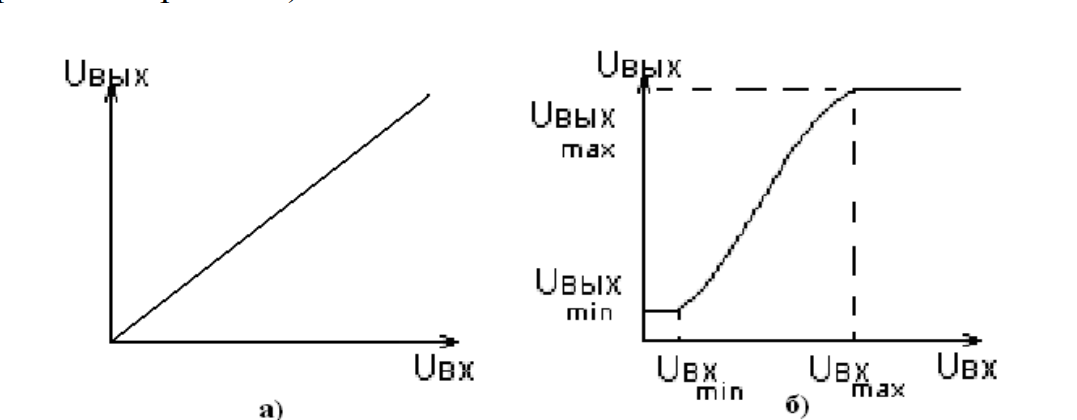
\includegraphics[width=0.8\linewidth]{figs/def_pa_char.png}
    \caption{Амплитудные характеристики идеального и реального усилителя мощности}
    \label{fig:1.1}
\end{figure}

Однако как наблюдается на практике, АХ усилителей редко бывают линейными,
ввиду множества факторов, обуславливающих нелинейность этой характеристики
(см. Рис. \ref{fig:1.1}б). При нулевом напряжении на входе, на выходе
усилителя присутствует ненулевое напряжение, обусловленное собственными
шумами усилителя. Из-за этого появляется изгиб в нижней части АХ. При
достаточно больших значениях входной амплитуды, АХ также отклоняется от
прямой. Из-за выхода рабочей точки отдельных элементов усилителя за пределы
рабочего диапазона, возникают нелинейные искажения, в следствие которых
коэффициент усиления сигнала выходит на уровень насыщения.

При этом, АХ реального УМ имеет определенный диапазон входных значений
амплитуд $(U_{in}^{min},U_{in}^{max},)$, при которых искажения практически
отсутствуют и усилитель подобен идеальному. Эта область называется
\textit{динамическим диапазоном усилителя} и выражается как
\begin{equation}
    D = \frac{U_{in}^{max}}{U_{in}^{min}}.
\end{equation}

В связи с ограниченностью динамического диапазона УМ, часто изменяют
входной сигнал таким образом, чтобы итоговая рабочая точка находилась в
нужном диапазоне линейности и усиления. Используется смещение рабочей точки
относительно выходной мощности - OBO (\textit{Англ. - Output back-off}), и
смещение рабочей точки относительно входной мощности - IBO (\textit{Англ. -
Input back-off}). При этом обычно представляется возможным пересчет одной
величины в другую, так как по сути они являются взаимозаменяемыми. Разница
состоит в том, относительно чего происходит сдвиг рабочей точки -
максимальной выходной, либо максимальной входной мощности.

\begin{figure}[h!]
    \centering
    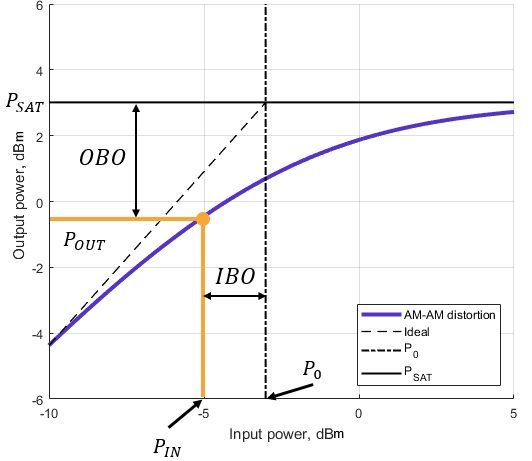
\includegraphics[width=0.7\linewidth]{figs/pa_obo_ibo.png}
    \caption{Смещение рабочей точки усилителя относительно входной и выходной мощности}
    \label{fig:1.2}
\end{figure}

\begin{equation}
    OBO = 10 \cdot \log_{10}\left(\frac{P_{sat}}{P_{out}}\right), \quad
    IBO = 10 \cdot \log_{10}\left(\frac{P_{0}}{P_{in}}\right)
\end{equation}

Большие значения IBO\slash OBO могут обеспечить хорошую линейность АХ,
однако это также приведет к уменьшению средней выходной мощности сигнала.
Таким образом, в реальных применениях определяется наиболее подходящее
значение IBO \slash OBO, обеспечивающее необходимую линейность
характеристики, а также необходимое усиление.


\subsection{Нелинейность и искажение сигналов}
Мощность на выходе УМ увеличивается вместе с ростом входной мощности,
однако, как только уровень выходной мощность достигает определенного
максимума, КУ перестает быть постоянным и УМ входит в область насыщения. В
этой области больше всего проявляется нелинейность УМ - выходная мощность
перестает увеличиваться с ростом входной мощности. Работа УМ в нелинейной
области влечет за собой нелинейные искажения сигнала, которые заключаются в
изменение его формы и фазы.

Рассмотрим в качестве входного сигнала гармонический (синусоидальный)
сигнал (см. рис \ref{fig:pa_distortion_sin}). Если УМ находится в линейном
режиме работы, то на выходе также будет синусоида, отличающаяся только
усилением амплитуды. Однако если усилитель находится в нелинейной области,
на выходе сигнал будет отличаться от входного не только значением
амплитуды, но и формой. Пики синусоиды будут сжиматься нелинейной частью
АХ, что приведет к искажению сигнала на выходе.

\begin{figure}[h!]
    \centering
    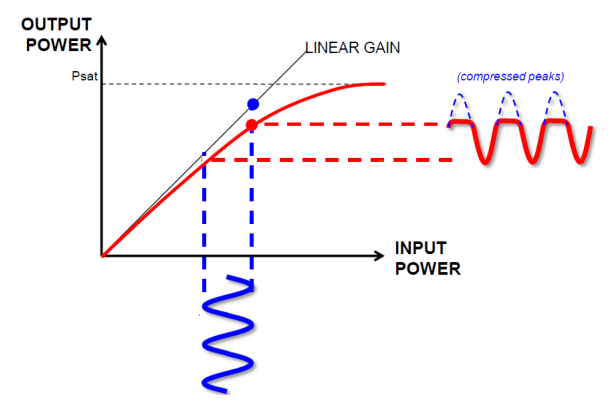
\includegraphics[width=0.7\linewidth]{figs/example_pa_signal.png}
    \caption{Преобразование сигнала при прохождении через УМ}
    \label{fig:pa_distortion_sin}
\end{figure}

Сжатие пиков во временной области будет также приводить к искажениям и 
изменениям в частотной
области, а именно к росту ширины спектра. Изначально подаваемый сигнал
имеет очень узкий спектр (дельта-функция на несущей частоте) 

\begin{figure}[h!]
    \centering
    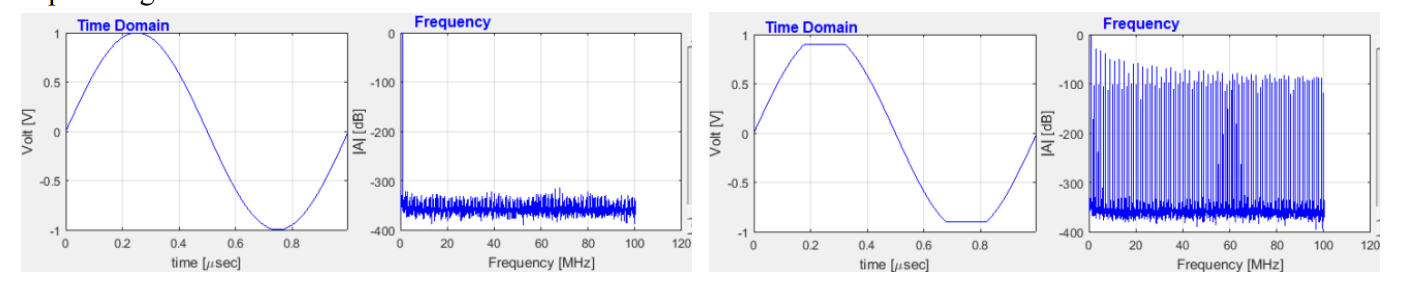
\includegraphics[width=0.9\linewidth]{figs/pa_spectral_growth.png}
    \caption{Влияние сжатия пиков на частотную область сигнала}
    \label{fig:pa_distortion_freq}
\end{figure}

\subsubsection{SC}
\subsubsection{OFDM}
\subsubsection{DFT-s-OFDM}
% Тут про SC-OFDM, CP-OFDM, бла бла бла
% Или все-таки описать это когда ofdm сигнал опишу?



\subsection{Математическое описание характеристик реальных УМ}

Для моделирования использования УМ в системах мобильной связи часто прибегают к
математическим моделям, описывающим поведение сигнала (усиление, искажение) при 
прохождении через УМ. Исторически модели разделяются на две основных
группы - \textbf{физические} и \textbf{эмпирические} модели \cite{cambridge2008}.

Физические модели требуют знания внутренних электронных компонентов УМ, их
связи, а так же теории, описывающей их взаимодействие. Такие модели подходят
для симуляций на уровне схемы благодаря высокой точности, однако требуют
много вычислительных мощностей и времени, а также детальное описание
структуры и компонентов УМ.

Эмпирические модели используются, когда не известна внутренняя структура УМ,
или когда рассматривается системный уровень моделирования. Эти модели
основаны на результатах измерений и исследований конкретных УМ, на основе
которых были выведены зависимости снятых характеристик УМ (АХ, ФХ) от его
параметров.

Поскольку в данной работе исследуется возможность компенсации нелинейного
искажения на приемнике, то использоваться будет эмпирическая
(поведенческая) модель УМ. Среди таких моделей можно назвать
\textit{Volterra, Saleh, Ghorbani}, а также модели, представляющие собой комбинации
полиномиальных моделей. Все они являются достаточно простыми моделями,
которые отражают нелинейную природу УМ. Простота позволяет оперировать
меньшим количеством параметров усилителя, упрощая обработку в целом. Однако
такие модели не могут быть использованы для описания сложных усилителей,
таки как усилитель \textit{Doherty} \cite{Doherty1936}\cite{3gpp.38.803}.

С другой стороны, в рамках рассматриваемой задачи, а именно компенсации
искажений, внесенных на передатчике из-за нелинейности УМ, использование
более простой модели может быть оправдано. Целью данной работы является
создание метода компенсации нелинейных искажений на приемнике, с основным
мотивом минимизировать обработку на передатчике, а также стоимость
конечного устройства. Рассматриваются именно простые, мало размерные,
дешевые в производстве передатчики, в которых усилитель часто имеет далеко
не лучшие параметры и не отличается высокой эффективностью.

\subsubsection{Модель Раппа}
Для описания искажения амплитуды и фазы при использовании твердотельных УМ
широко используется модель Раппа (\textit{Англ. - Rapp}) \cite{Rapp1991}.
Также существует модифицированная модель Раппа, приведенная в выражении
\ref{eq:Rapp}. Данная модель УМ включена в список моделей в спецификации
3GPP \cite{3gpp.38.803}.

\begin{equation}
    F_{AM/AM}(x) = \frac{G x}{\left( 1 + \abs{\frac{Gx}{V_{sat}}}^{2p}\right)^{1/2p}},
    \quad 
    F_{AM/PM}(x) = \frac{Ax^q}{\left(1+\left(\frac{x}{B}\right)^q\right)},
    \label{eq:Rapp}
\end{equation}
где $F_{AM/AM}, F_{AM/PM}$ - амплитудные и фазовые характеристики
соответственно, $G$ - КУ слабого сигнала, $V_{sat}$ - амплитуда насыщения,
$p$ - показатель гладкости характеристики. Параметры $A,B,q$ - параметры
кривой искажения фазы. В дальнейшем в работе будет использоваться эта
модель для описания влияния УМ на сигнал.

Пример АХ и ФХ для модели Раппа приведены на  рис. \ref{fig:rapp_p_parameters}.
В зависимости от значений параметров $G, V_{sat}, p$ поведение амплитудной
характеристики может сильно варьироваться. Так, при больших значениях $p$
($p\gg 1$), АХ похожа на характеристику идеального УМ, которая ограничена
по максимальной выходной амплитуде (см. рис.\ref{fig:rapp_p_parameters}).
Параметр $V_{sat}$ отвечает за выходную амплитуду насыщения, а $G$ - КУ
слабого сигнала, который показывает, как усилился бы сигнал, если бы УМ был 
идеальным.
\begin{figure}[h!]
    \centering
    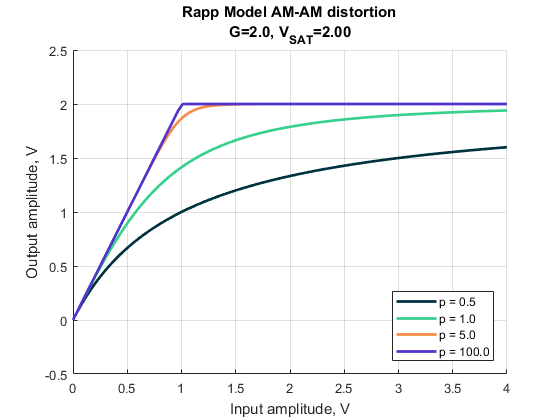
\includegraphics[width=0.7\linewidth]{figs/rapp_p.png}
    \caption{Влияние параметра гладкости $p$ на вид амплитудной
    характеристики (Добавить вторую и третью картинку где будут менять G, V)}
    \label{fig:rapp_p_parameters}
\end{figure}

\subsubsection{Параметры модели Раппа для диапазона 30-70 ГГц}
Для вывода параметров базовой модели УМ в диапазоне частот 30-70 ГГц,
компанией Nokia были использованы и исследованы характеристики стандартных
усилителей в соответствующей полосе \cite{nokia163314}. Полученная модель
УМ использована в этой работе для моделирования УМ в диапазоне частот 30-70
ГГц. Амплитудные и частотные характеристики УМ в соответствии с моделью
\cite{nokia163314} приведены на рис. \ref{fig:rapp_nokia}.

Численные значения параметров модели Раппа приведены ниже:
\begin{equation}
    G = 16, \quad V_{sat} = 1.9, \quad p = 1.41
\end{equation}

\begin{figure}[h!]
    \centering
    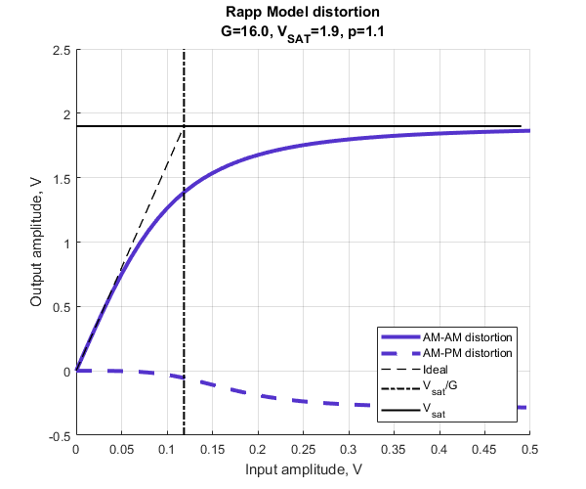
\includegraphics[width=0.7\linewidth]{figs/rapp_nokia.png}
    \caption{АХ и ФХ усилителя в соответствии с моделью Раппа и
    параметрами для диапазона 30-70 ГГц}
    \label{fig:rapp_nokia}
\end{figure}

\subsection{Характеристики УМ в миллиметровом диапазоне}
Помимо "базовой" модели УМ для диапазона 30-70 ГГц, интерес представляло
моделирование системы в миллиметровом диапазоне, а именно  в диапазоне
частот 100-200 ГГц. Основываясь на работах
\cite{zhang2021}\cite{amadorey2018}\cite{aliyun2020} был сделан вывод о
значительном отличии характеристик УМ в более высоком диапазоне частот.

Характеристики усилителей из исследований приведены на рис.
\ref{fig:pa_research_mean}. Также на рис. \ref{fig:pa_research_mean}
приведены модель для 30-70 ГГц.
\begin{figure}[h]
    \centering
    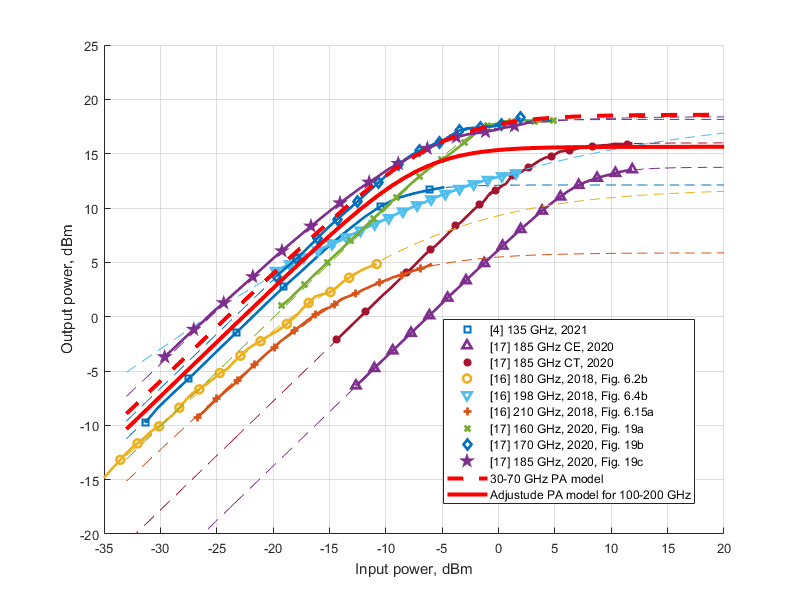
\includegraphics[width=0.7\linewidth]{figs/pa100mean.png}
    \caption{АХ усилителей на основе данных из
    \cite{zhang2021}\cite{amadorey2018}\cite{aliyun2020}, а также
    полученная усредненная модель для диапазона 100-200 ГГц}
    \label{fig:pa_research_mean}
\end{figure}

Извлеченные кривые амплитудных характеристик были аппроксимированы при
помощи модели Раппа \ref{eq:Rapp}, что позволило собрать параметры УМ для
дальнейшей обработки. Полученные значения, а также частота и технология
для рассматриваемых УМ приведены в Таблице \ref{tab:pa_params}. 

\begin{table}[h]
    \centering
    \begin{tabular}{llcccc}
        \hline
    Источник              & Технология   & Частота, ГГц & $G$  & $V_{sat}$ & $p$ \\ \hline
    \cite{zhang2021}      & 28-нм CMOS   &  135         & 12.26 & 0.9      & 1.93  \\
    \cite{amadorey2018} Рис. 6.2b  & 35-нм mHEMT      &  180  & 10.84 & 0.87 & 0.52 \\
    \cite{amadorey2018} Рис. 6.4b  & 50-нм mHEMT      &  198  & 41.19 & 1.99 & 0.26  \\
    \cite{amadorey2018} Рис. 6.15a & 35-нм GaAs mHEMT &  210  & 7.89  & 0.44 & 0.9  \\
    \cite{aliyun2020} CT       &  130-нм SiGe BiCMOS CT        & 185 & 2.05  & 1.09 & 2.03  \\
    \cite{aliyun2020} CE       & 130-нм SiGe BiCMOS CE         & 185 & 4.08  & 1.41 & 1.91  \\
    \cite{aliyun2020} Рис. 19a & 130-нм SiGe BiCMOS 3-stage CT & 160 & 9.88  & 1.81 & 2.75  \\
    \cite{aliyun2020} Рис. 19b & 130-нм SiGe BiCMOS 3-stage CT & 170 & 14.8  & 1.81 & 1.56  \\
    \cite{aliyun2020} Рис. 19c & 130-нм SiGe BiCMOS 3-stage CT & 185 & 19.29 & 1.86 & 0.87  \\\hline
    \end{tabular}
    \caption{Параметры модели Раппа для УМ в диапазоне частот 100-200 ГГц
    на основе экспериментальных данных и исследований}
    \label{tab:pa_params}
\end{table}

\subsubsection{Новая модель для диапазона частот 100-200 ГГц}
Для исследования применимости нового метода компенсации в диапазоне 100-200
ГГц необходима соответствующая модель УМ, для начальной имплементации ее в
систему с целью внесения соответствующих искажений в сигнал, и последующей
компенсацией внесенных искажений на приемнике. 

Имеющаяся модель \cite{nokia163314} подходит только для диапазона  30-70
ГГц, в нашем случае интерес представляет работа при более высоких частотах.
Модель для 100-200 ГГц была создана путем усреднения параметров $G,
V_{sat}, p$ рассмотренных УМ в соответствующем диапазоне частот (см. Талбицу
\ref{tab:pa_params}). Полученные усредненный параметры для модели Раппа
приведены ниже:
\begin{equation}
    G = 13.59, \quad V_{sat} = 1.35, \quad p = 1.41
\end{equation}



\section{Метод компенсации нелинейных искажений на приемнике}
Компенсация нелинейных искажений сигнала является важным этапом для
сохранения производительности системы. С расширением стандарта связи 5G NR
в миллиметровый диапазон, компенсация становится особенно актуальной,
поскольку характеристики усилителей в этом диапазоне значительно хуже, чем
для более низких частот.

\subsection{Обзор существующих решений}
На текущий момент были исследованы несколько основных подходов для
компенсации нелинейных искажений, они разделяются на два основных
направления. Первый заключается в предварительном искажении сигнала перед
подачей на УМ на передатчике. Сигналу придаются свойства, которые
минимизируют влияние нелинейного искажения от УМ, эффективно "выпрямляя"
его АХ. Существует множество вариантов обработки для данного подхода,
однако многие из них имеют слабый эффект на общей производительности
системы, а подход с применением предварительного искажения сигнала имеет
низкую эффективность при низких значениях IBO, при которой достигается
максимальная эффективность усилителя \cite{sharath2015}
\cite{shabany2008} \cite{eda2001}. Также, использование PD на передатчике
нежелательно на мало-габаритных устройствах, поскольку в таком случае
увеличивается сложность устройства, объем сигнальной обработки и энергопотребление.


Второй основной подход заключается в компенсации нелинейных искажений на
приемнике. Например, в работе \cite{maltsev2021} используется
статистическая обработка принятого сигнала для определения степени
искажения, на основе которой в дальнейшем производится компенсация. Многие
работы \cite[]{sharath2015, shabany2008,bhat2016,qi2010,gregorio2007,
bouhadda2015,drotar2010} рассматривают теоретический подход для компенсации
на приемнике в очень обобщенном случае. Несколько методов компенсации были
предложены для OFDM сигнала \cite[]{gregorio2007,bouhadda2015, drotar2010},
где влияние нелинейности представляется комплексным множителем, а также
Гауссовой шумовой компонентой. Основной задачей в таком случае является
определение параметров УМ (они могут быть как известны изначально, так и
определены с помощью пилотных сигналов) для компенсации нелинейного
искажения. Несколько методов были исследованы для сигнала SC с одной несущей
(\textit{Англ. - SC - Single Carrier}) \cite[]{sharath2015,
shabany2008,bhat2016, qi2010}, в частности использовалась обратная
характеристика УМ и последовательные методы Монте-Карло. В нескольких
случаях \cite[]{bhat2016, qi2010,gregorio2007}, значения параметров УМ
считаются известными на приемнике, что позволяет произвести компенсацию
искажения. В случаях, когда параметры УМ оцениваются, производительность
такая же либо хуже.

В данной работе описывается метод компенсации нелинейных искажений УМ на
приемнике с использованием обратной амплитудной характеристики. Информация
о параметрах и рабочей точке усилителя предполагается известной. Работа и
эффективность метода будет исследоваться на существующем симуляторе
канального уровня, необходимые изменения будут вноситься в код симулятора
как для внесения искажений, так и для их компенсации.



\subsection{Краткое описание архитектуры LLS}

Для исследования влияния нелинейности УМ в диапазонах частот 30-70 ГГц и
100-200 ГГц, а также проверки работоспособности разработанного метода
компенсации нелинейных искажений на приемнике, в работе использовался
полноценный симулятор канального уровня LLS (\textit{Англ. - Link Level
Simulator}), соответствующий требованиям стандарта 5G NR 3GPP. В этой части
работы будут кратко описаны принципы работы, архитектура и основные
составляющие LLS. 

На рис. \ref{fig:lls_scheme} приведена принципиальная схемы работы LLS.
\begin{figure}[h!]
    \centering
    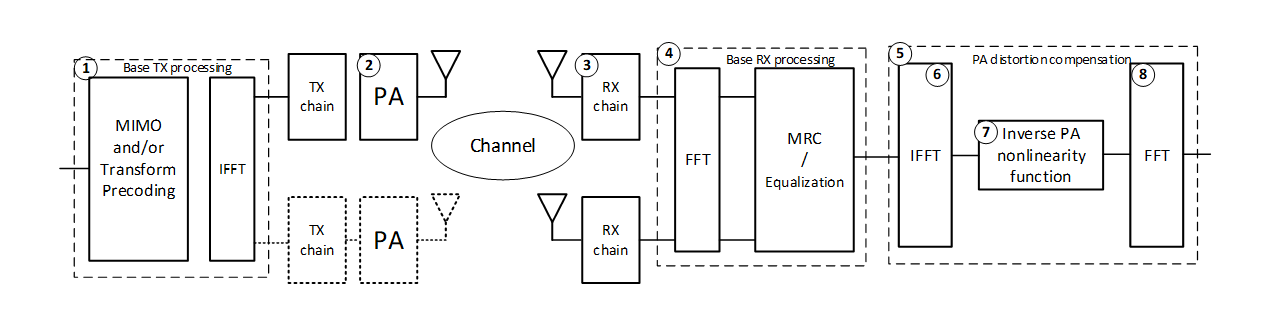
\includegraphics[width=0.99\linewidth]{figs/lls_scheme.png}
    \caption{}
    \label{fig:lls_scheme}
\end{figure}

TBD

% Схема компенсации состоит из базовой обработки на передатчике (1),
% которая может включать MIMO прекодинг и transform прекодинг (в случае
% DFT-s-OFDM сигнала),  а также стандартного для OFDM блока обратного
% преобразования Фурье. Сгенерированный OFDM сигнал подается на одну или
% более передающих цепочек, которые могут включать добавление цикличного
% префикса, перенос сигнала на несущую частоту, и, наконец, сигнал подается
% на усилитель мощности (2), работающий на несущей частоте. Отметим, что
% для корректной работы предлагаемой схемы, сигналы на разных антеннах
% должны иметь одинаковую амплитуду (но могут иметь разную фазу). Это
% ограничивает применение данного метода до передачи 1 ранга, даже если
% используется несколько передающих антенн. После прохождения через канал,
% сигнал попадает на приемную цепь состоящую из одной или нескольких
% приемных антенн для дальнейшей обработки (4), которая может состоять из
% преобразования Фурье further maximum ration combining (MRC) and frequency
% domain equalization???. Такая обработка эффективно нивелирует влияние
% частотно-селективного канала, что позволяет использовать обработанный
% сигнал на блоке компенсации нелинейного искажения (5). Этот блок может
% состоять из операции обратного Фурье преобразования (6) для возвращения
% сигнала во временную область, блока обратной нелинейной функции УМ (7),
% который выполняет компенсацию нелинейного искажения, а также блока
% прямого преобразования Фурье для возвращения сигнала в частотную область.






\subsection{Влияние нелинейных искажений в LLS}

\begin{figure}[h!]
    \centering
    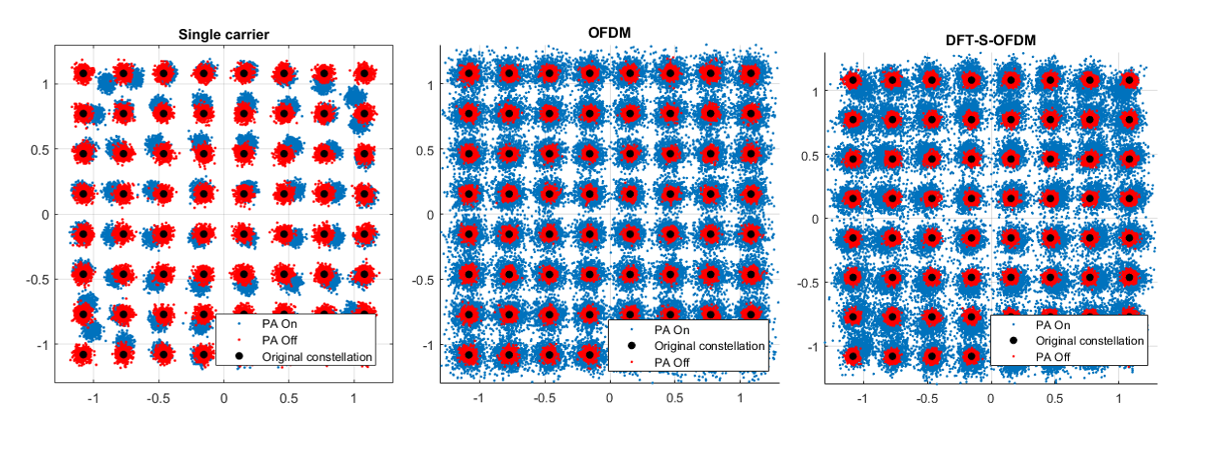
\includegraphics[width=0.95\linewidth]{figs/ofdm_pa_distortions.png}
    \caption{Искажение различных сигналов на приемнике при внесении нелинейного
    искажения на передатчике}
    \label{fig:lls_rapp_distortions}
\end{figure}

\subsection{Подход и описание нового метода компенсации нелинейных искажений}
В основе разработанного метода компенсации нелинейных искажений на
приемнике лежит использование обратной АХ усилителя. Параметры $G, V_{sat},
p$, необходимые для восстановления обратной характеристики считаются
известными. Помимо этих параметров, важно также знать рабочую точку УМ,
поскольку это напрямую влияет на степень искажения принятого сигнала.
Рабочая точка также считается известной.

Принципиальный подход компенсации искажений может быть описан следующим
образом:
\begin{enumerate}
    \item Принятый сигнал проходит через предварительную обработку в LLS
    (частотное выравнивание, MIMO-декодирование, перенос в частотную
    область)
    \item Полученный обработанный сигнал в частотной области переносится во
    временную область в соответствии с используемым типом сигнала.
    \subitem Transform precoding (в случае DFT-s-OFDM сигнала)
    \subitem IFFT-обработка для получения OFDM сигнала во временной области
    \item Полученный сигнал во временной области подается на блок
    компенсации (использующий обратную АХ усилителя на основе известных
    параметров и рабочей точки)
    \item Сигнал с компенсированными искажениями переводится в частотную
    область
    \item Компенсированный сигнал подается на блок демодуляции
\end{enumerate}

Блок-схема разработанного метода компенсации приведена на рис.
\ref{fig:compensation_scheme}. 

\begin{figure}[h!]
    \centering
    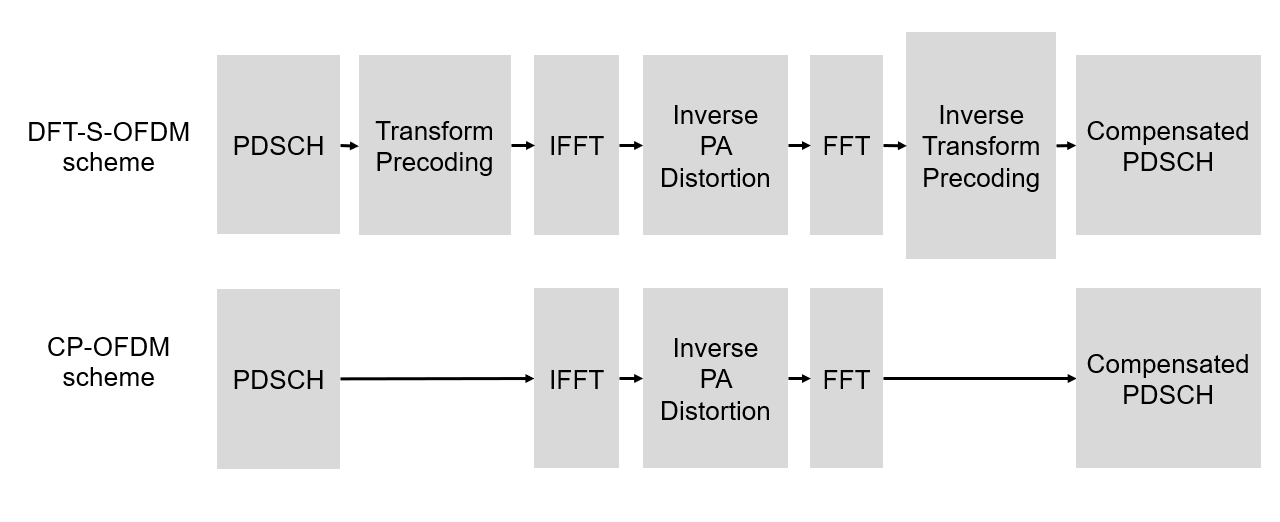
\includegraphics[width=0.95\linewidth]{figs/compensation_scheme.png}
    \caption{}
    \label{fig:compensation_scheme}
\end{figure}

\begin{equation}
    F^{-1}_{AM/AM}(y) = 
    \begin{cases}
        \displaystyle
       \frac{ y}{\left( 1 - \abs{\frac{y}{V_{sat}}}^{2p}\right)^{1/2p}}
       \quad y <\alpha V_{sat}\\
       \frac{ \alpha V_{sat}}{\left( 1 - \abs{\alpha}^{2p}\right)^{1/2p}}
       \quad y \geq \alpha V_{sat}
    \end{cases},
    \label{eq:invRapp}
\end{equation}

TBD



\subsubsection{Компенсация с использованием обратной характеристики усилителя}
Тут написать про обратную характеристику, приколы возникающие при ее
неограничении и как она используется для компенсации.

\subsubsection{Адаптация алгоритма компенсации в зависимости от типа используемого сигнала}
Возможность обработки нескольких типов сигнала в зависимости от типа
сигнала.
\section{Результаты}
\label{sec:results}
Для проверки эффективности разработанного метода компенсации нелинейных
искажений на приемнике, с помощью LLS были произведены симуляции канального
уровня, в которых предложенный метод сравнивался со случаями идеального УМ,
а также отсутствии компенсации на приемнике для совпадающей модели
усилителя. Использовалась модель основанная на параметрах существующих
усилителей мощности в диапазоне частот 30-70 ГГц \cite{nokia163314}, а
также модель для 100-200 ГГц \ref{eq:rapp_p100200} полученная в результате
данной работы.

Симуляции проводились в системе Matlab, все описанные алгоритмы компенсации
также были имплементированы на языке Matlab.

Расчеты проводились для различных параметров системы, таких как расстояние
между поднесущими (SCS), типом используемого сигнала, кодирование,
модуляция и другие. перечень всех используемых параметров симуляций
приведен в таблице \ref{tab:lls_parameters}.
\begin{table}[h!]
    \centering
    \bgroup
    \def\arraystretch{1.5}
    \begin{tabular}{l|p{0.4\linewidth}}
    Параметр & Используемые значения \\ \hline
    Несущая частота, $f_c$ & 60 ГГц   \\ \hline
    Полоса частот &  400 МГц  \\ \hline
    Тип сигнала &  CP-OFDM, DFT-s-OFDM  \\ \hline
    Модель УМ  &  Модель 30-70 ГГц \cite{nokia163314}, модель 100-200 ГГц \ref{eq:rapp_p100200}   \\ \hline
    Мощность $P_{TX}$ &  10 dBm  \\ \hline
    SCS &  120, 480, 960 кГц  \\ \hline
    $N_{RB}$ &  256, 64, 32  \\ \hline
    Модель канала &  TDL-A, 5 нс DS, 3 км/ч  \\ \hline
    Параметры антенн &  1 TX, 2 RX MRC  \\ \hline
    Модуляция и кодирование &  64-QAM (MCS Таблица 1: 22, 27), 256-QAM (MCS Таблица 2: 22)  \\ \hline
    Помехи &  Фазовый шум (BS and UE example 2 model \cite{3gpp.38.803}),
    компенсирован LS фильтром. Оценка канала - LS fitting per precoding
    region (24subc)
    % TBD!!!.   
    \end{tabular}
    \egroup
    \caption{Параметры и допущения LLS, использованные при моделировании}
    \label{tab:lls_parameters}
\end{table}

В качестве метрики, с помощью которой производилась оценка эффективности,
использовалось отношение числа поврежденных ошибками блоков $N^B_{error}$ к общему числу
блоков $N^B$: $BLER = N^B_{error} / N^B$ (\textit{Англ. - Block Error
Rate}). Блок считается поврежденным, если в ходе передачи было повреждено
или неверно декодировано больше определеннго количества бит. BLER измерялся
в зависимости от SNR.

\subsection{Результаты симуляций для модели 30-70 ГГц}
В данной секции приведены результаты моделирования для модели УМ 30-70 ГГц. 
На рис. \ref{fig:res3070_scs120} - \ref{fig:res3070_scs960} приведены
зависимости BLER от SNR для различных значений SCS и MCS.
\begin{figure}[h!]
    \centering
    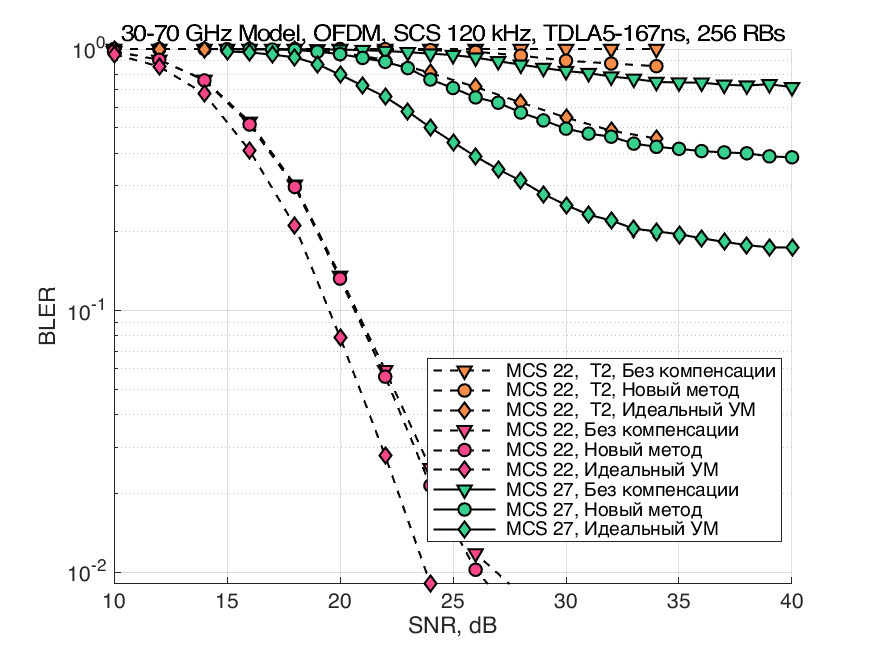
\includegraphics[width=0.49\linewidth]{figs/res/ofdm/OFDM_Nokia_SCS120_MCS22_27.png}
    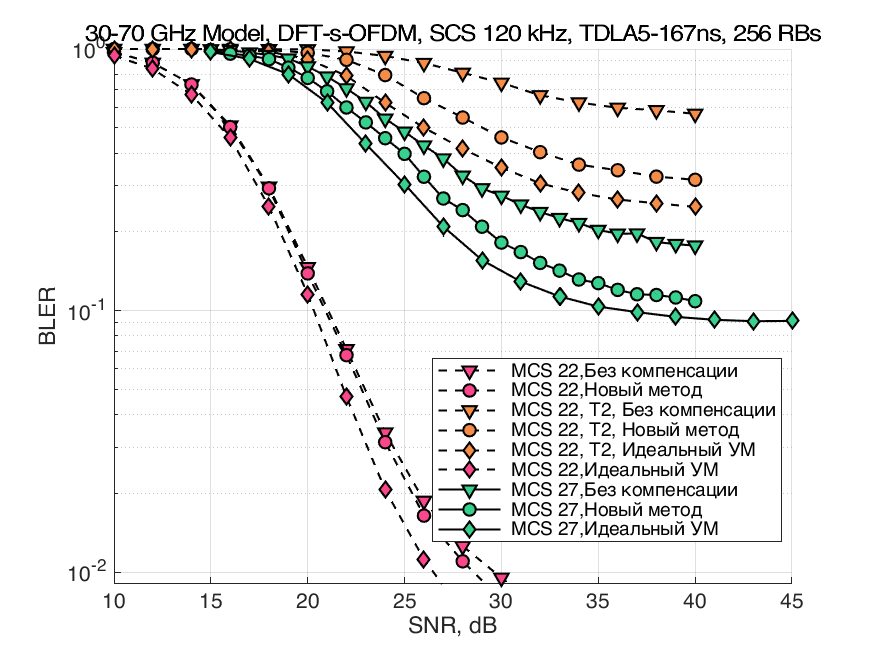
\includegraphics[width=0.49\linewidth]{figs/res/dftsofdm/DFT-s-OFDM_Nokia_SCS120_MCS22_27.png}
    \caption{BLER для SCS 120 кГц, 64-QAM/256 QAM для OFDM (слева) для DFT-s-OFDM(справа)}
    \label{fig:res3070_scs120}
\end{figure}

\begin{figure}[h!]
    \centering
    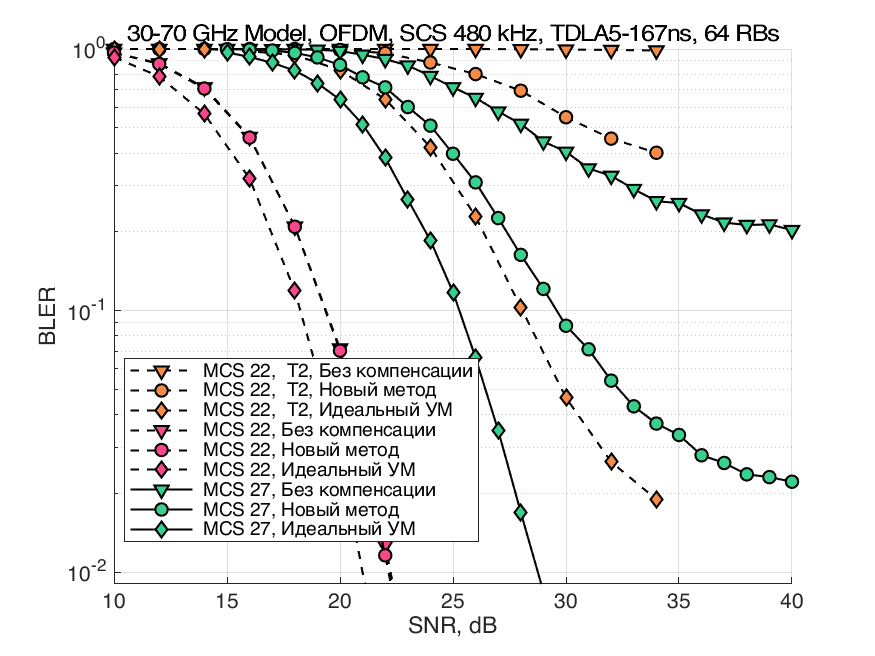
\includegraphics[width=0.49\linewidth]{figs/res/ofdm/OFDM_Nokia_SCS480_MCS22_27.png}
    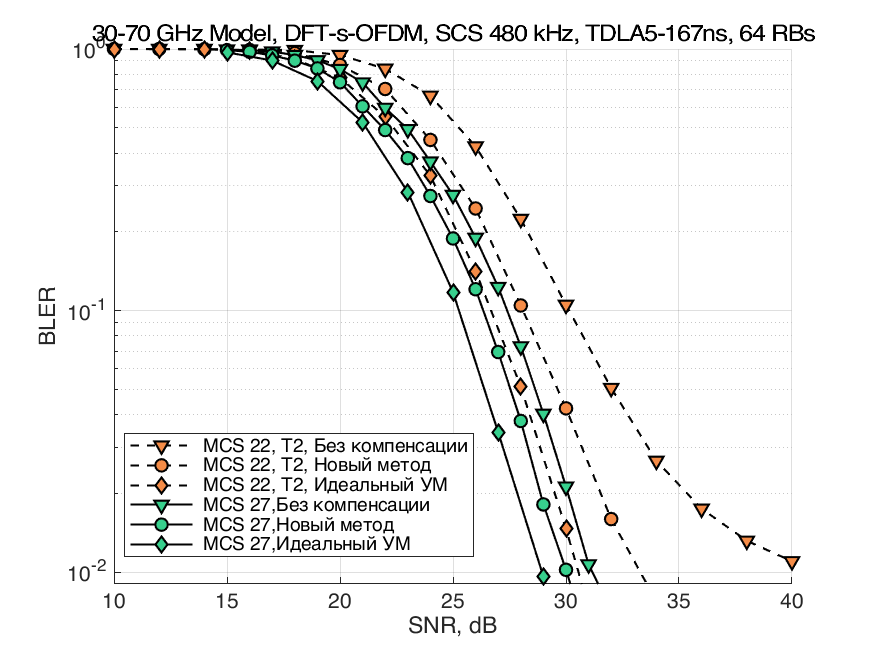
\includegraphics[width=0.49\linewidth]{figs/res/dftsofdm/DFT-s-OFDM_Nokia_SCS480_MCS22_27.png}
    \caption{BLER для SCS 480 кГц, 64-QAM/256 QAM для OFDM (слева) для DFT-s-OFDM(справа)}
    \label{fig:res3070_scs480}
\end{figure}

\begin{figure}[h!]
    \centering
    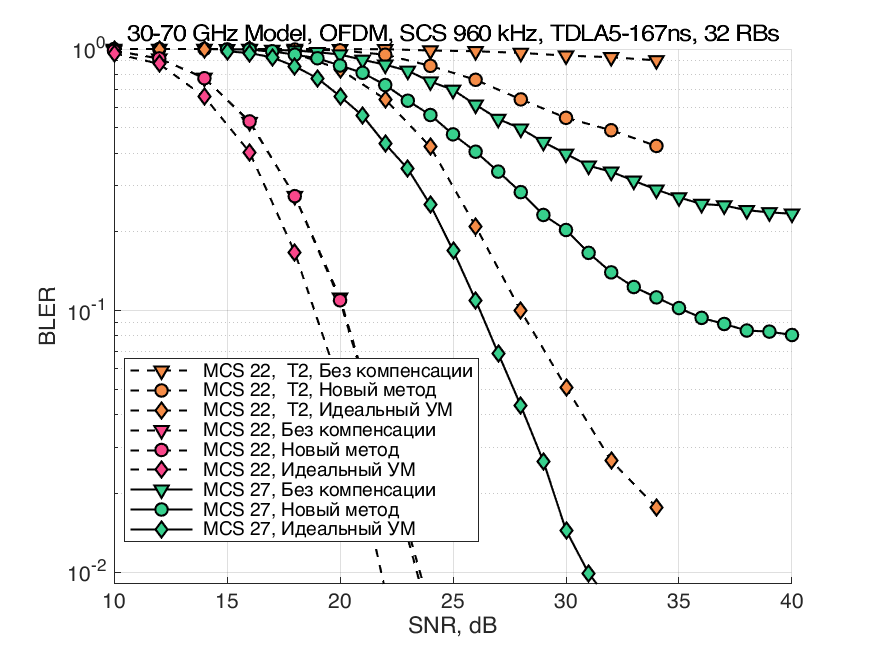
\includegraphics[width=0.49\linewidth]{figs/res/ofdm/OFDM_Nokia_SCS960_MCS22_27.png}
    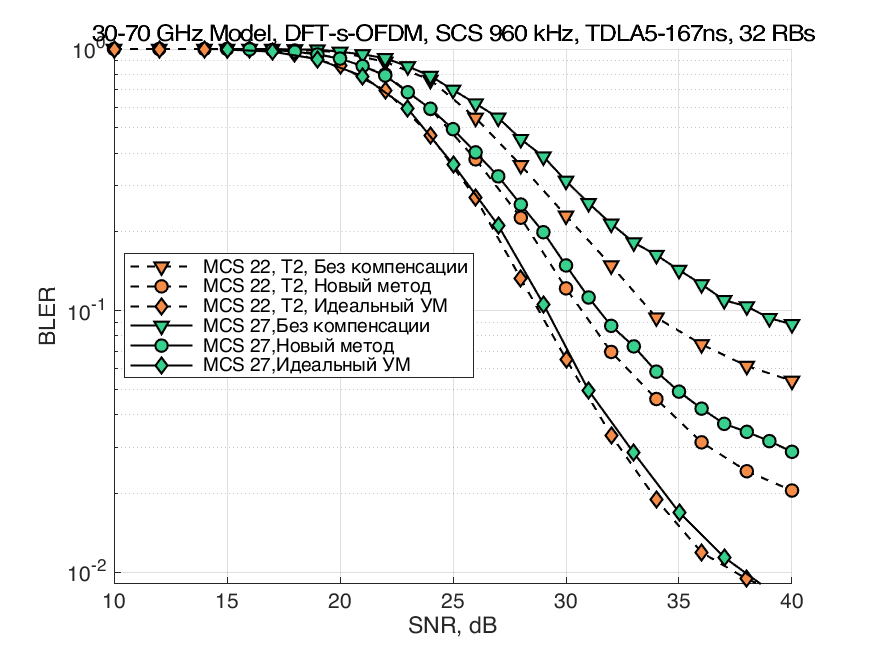
\includegraphics[width=0.49\linewidth]{figs/res/dftsofdm/DFT-s-OFDM_Nokia_SCS960_MCS22_27.png}
    \caption{BLER для SCS 960 кГц, 64-QAM/256 QAM для OFDM (слева) для DFT-s-OFDM(справа)}
    \label{fig:res3070_scs960}
\end{figure}

Кратко опишем полученные результаты. Как и ожидалось, при добавлении
нелинейности УМ в работу LLS, кривая зависимости BLER от SNR стала выше.
Это значит что при том же уровне SNR, количество блоковых ошибок
увеличилось. Например, на рис. \ref{fig:res3070_scs480}(справа)
BLER при SNR$=25$ dB для MCS 27 в случае идеального УМ составлял
$BLER\simeq 10^{-1}$. При добавлении нелинейности УМ, BLER вырос до
$\simeq 3\cdot10^{-1}$. При использовании нового метода компенсации, BLER
понизился до $\simeq 2\cdot10^{-1}$.

Для модели УМ в диапазоне 30-70 ГГц (подходящего для диапазона FR2)
улучшение наблюдается в основном только для модуляций высокого порядка и
при высоких значениях SCS. В частности, для SCS 120 кГц (рис.
\ref{fig:res3070_scs120}), отрицательные эффекты присутствующего в LLS
фазового шума настолько значительны, что при таких искажениях результаты
компенсации нелинейности УМ практически не играют роли. Для высоких
модуляций уровень BLER выравнивается не достигнув значения $10^{-1}$, что
означает плохую производительность системы в целом. Однако даже в таких
условиях можно наблюдать улучшение результатов - кривые BLER в случае
компенсации смещаются на несколько dB по сравнению с случаем отсутствия
компенсации.

Для SCS 480 и 960 кГц (рис. \ref{fig:res3070_scs480},
\ref{fig:res3070_scs960}), в которых возможна более эффективная компенсация
фазового шума, в определенный момент влияние нелинейности УМ становится
основным ограничивающим фактором. В этом случае компенсация нелинейности УМ
может улучшить результат на несколько dB.

\subsection{Результаты симуляций для модели 100-200 ГГц}
В данной секции приведены результаты моделирования для модели УМ 100-200 ГГц. 
На рис. \ref{fig:res100200_scs120} - \ref{fig:res100200_scs960} приведены
зависимости BLER от SNR для различных значений SCS и MCS.

\begin{figure}[h!]
    \centering
    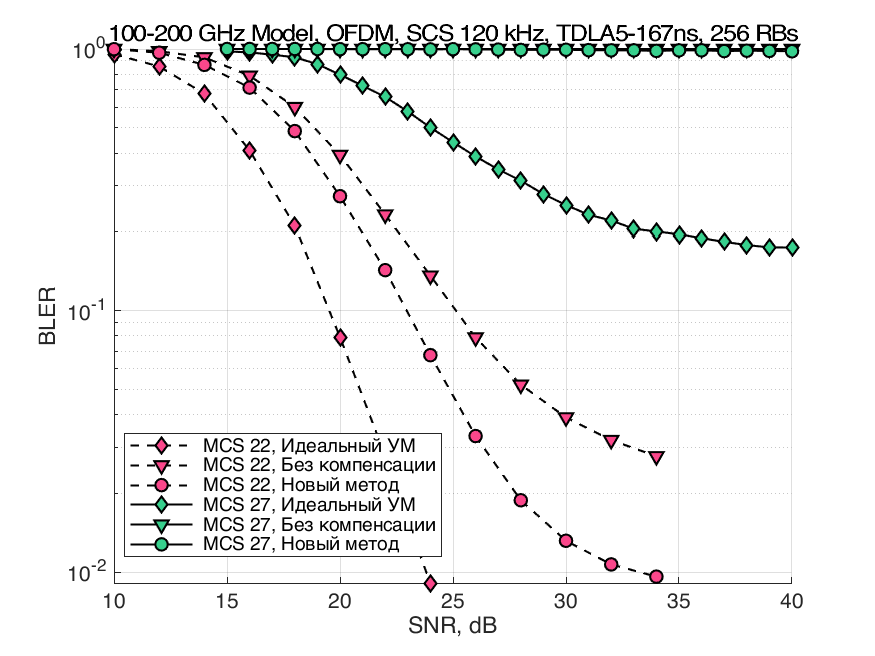
\includegraphics[width=0.49\linewidth]{figs/res/ofdm/OFDM_SubTHz_SCS120_MCS22_27.png}
    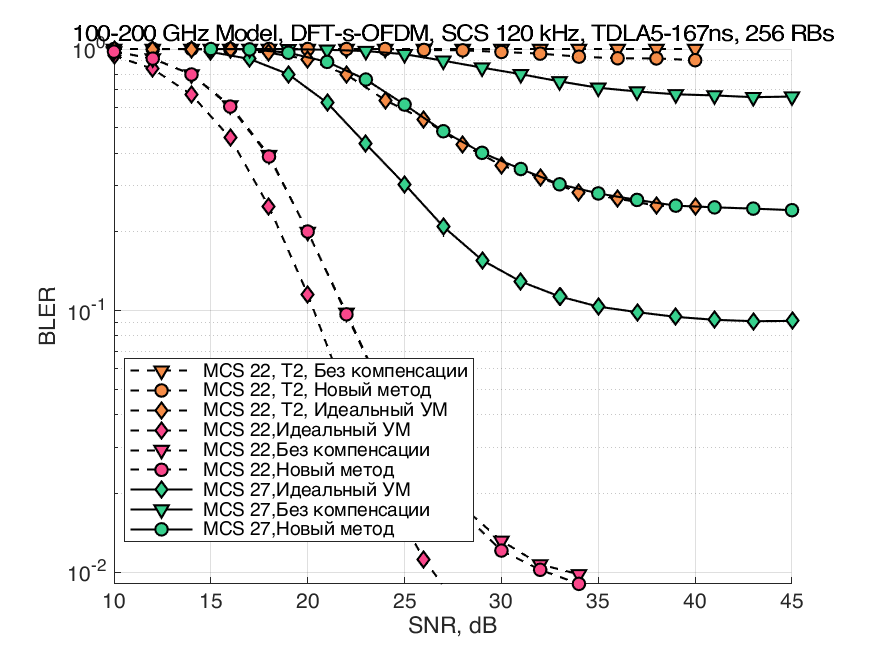
\includegraphics[width=0.49\linewidth]{figs/res/dftsofdm/DFT-s-OFDM_SubTHz_SCS120_MCS22_27.png}
    \caption{BLER для SCS 120 кГц, 64-QAM/256 QAM для OFDM (слева) для DFT-s-OFDM(справа)}
    \label{fig:res100200_scs120}
\end{figure}

\begin{figure}[h!]
    \centering
    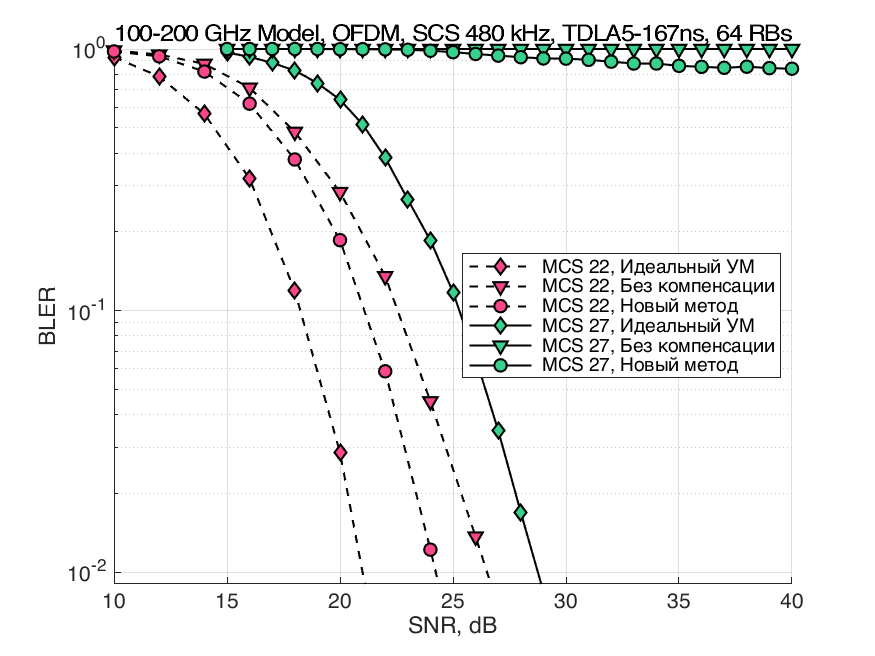
\includegraphics[width=0.49\linewidth]{figs/res/ofdm/OFDM_SubTHz_SCS480_MCS22_27.png}
    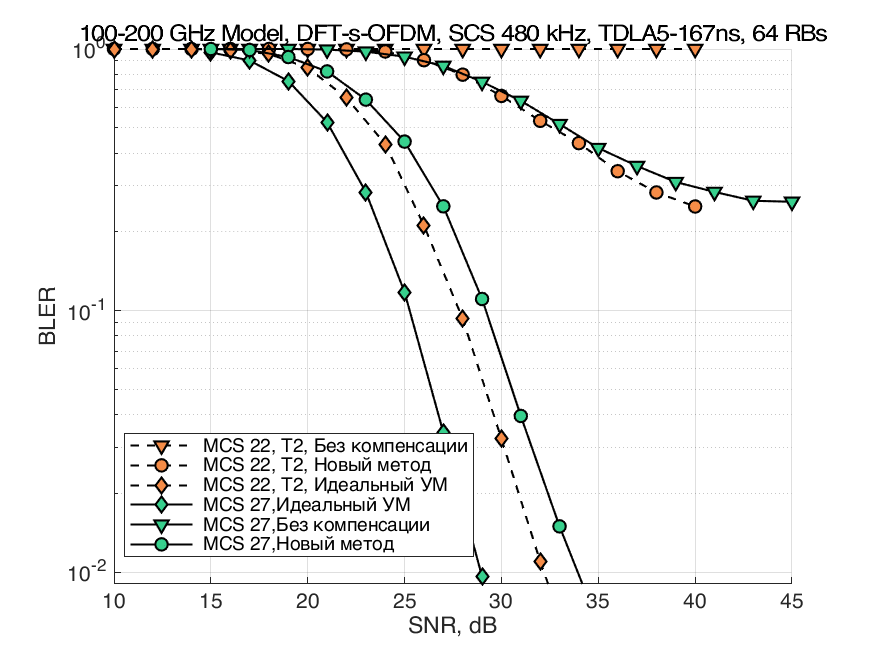
\includegraphics[width=0.49\linewidth]{figs/res/dftsofdm/DFT-s-OFDM_SubTHz_SCS480_MCS22_27.png}
    \caption{BLER для SCS 480 кГц, 64-QAM/256 QAM для OFDM (слева) для DFT-s-OFDM(справа)}
    \label{fig:res100200_scs480}
\end{figure}

\begin{figure}[h!]
    \centering
    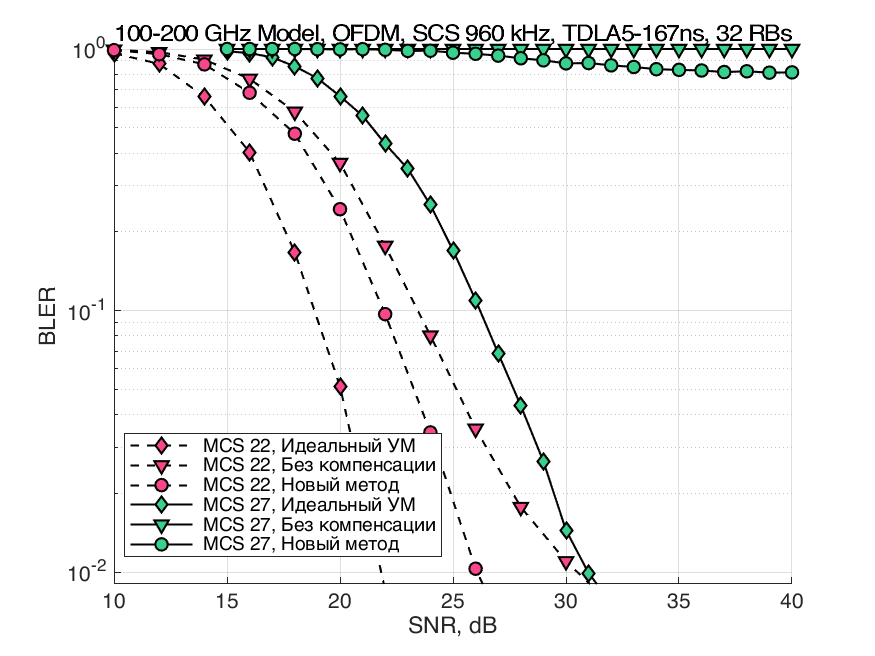
\includegraphics[width=0.49\linewidth]{figs/res/ofdm/OFDM_SubTHz_SCS960_MCS22_27.png}
    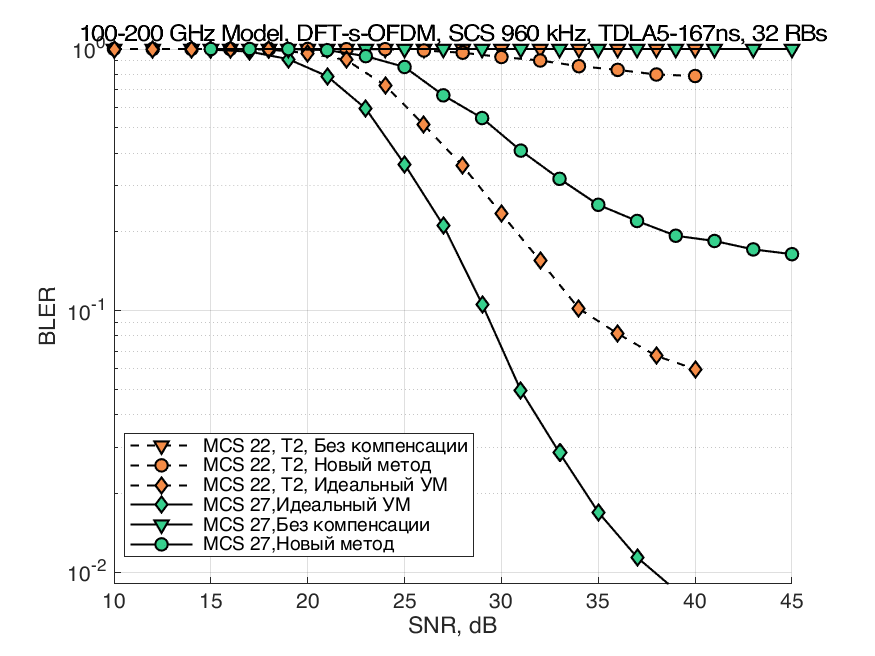
\includegraphics[width=0.49\linewidth]{figs/res/dftsofdm/DFT-s-OFDM_SubTHz_SCS960_MCS22_27.png}
    \caption{BLER для SCS 960 кГц, 64-QAM/256 QAM для OFDM (слева) для DFT-s-OFDM(справа)}
    \label{fig:res100200_scs960}
\end{figure}

Для модели 100-200 ГГц, влияние нелинейности УМ увеличивается, и в
большинстве случаев превосходит влияние фазовых шумов. Это связано с общим
ухудшением характирестик УМ в данном диапазоне, из-за чего происходят более
значительные искажения. В некоторых случаях, искажения настолько сильные,
что получение какой-либо информации практически невозможно, будь то с
компенсацией или без.

Предложенный метод компенсации демонстрирует улучшение результата для MCS
22 и выше как для сигнала DFT-s-OFDM, так и для сигнала CP-OFDM. В
большинстве случаев, при отсутствии эффекта насыщения кривой BLER,
разработанный метод улучшает результат на несколько dB. Например, для
сигнала OFDM SCS 120 кГц при MCS 22 рис. (\ref{fig:res100200_scs120}),
компенсация сдвинула результирующую кривую на 2-3 dB, при том что в
результате добавления нелинейности результат ухудшился на 5 dB. 

% Не смотря на возможность различных имплементаций, диктуемая логикой
% последовательность компенсации искажений в порядке, обратному их появлению
% в системе оказывается оптимальным. Таким образом, искажения должны быть
% компенсированы в порядке канал, усилитель мощности, фазовые шумы.  
% TBD


% % \chapter{Initial study of the problem via literature review and numerical simulations}


\section{Первоначальная постановка задачи и обзор литературы}
\label{cha:ch_1}

\section{Channel features affecting beam management}
\subsection{Channel features regarding AoA estimation}
Миллиметровая модель канала имеет ряд особенностей, которые описаны во множетстве
литературных источников и мировых стандартах \cite{Maltsev2010, Maltsev2017,
Xu2002, Akdeniz2014, Rappaport2015}. Основные особенности следующие:
\begin{itemize}
    \item Малое влияние дифракции и высокие потери на проникновении
    \item Высокие потери при распространении
    \item Потери на шероховатостях отражающих поверхностей
    \item Заметные потери в среде распространения (воздух, пар, дождь и др.)
    \item Пути распространения могут быть ассоциированы с геометрическими лучами
\end{itemize}

Последний пункт является наиболее важным с точки зрения алгоритмов оценки AOA.
Также, из этого свойства канала следует, что число
количество сильных путей распространения, которые могут быть обнаружены, относительно невелико. То есть
подтверждено результатами измерений каналов как для внутренних, так и для наружных сценариев.

Например, результаты измерения AOA для распространения в помещении
представлен на рис. \ref{fig:3.1}.

На рис. \ref{fig:3.2} представлены уникальные AOA в случае уличного сценария
Манхеттен. Можно заметить, что среднее число хорошо различимых независимых
путей распространения около 4-7 штук, что достаточно мало. 
На основе рассмотренных работ, можно сделать вывод, что в данной модели канала 
чаще всего всего можно выделить несколько сильнейших путей распространения и
определить их AOA.

\begin{figure}[h]
    \centering
    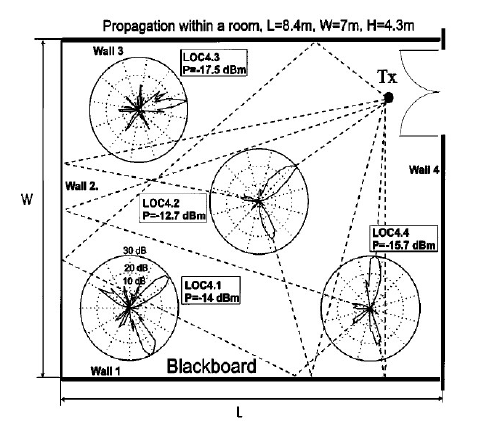
\includegraphics[width=0.8\linewidth]{figs/fig3.1}
    \caption{ Измерение AOA для определения пути распространения в помещении,
        измеренная мощность показана в полярных координатах, $P$ -- максимум
        измеренной мощности. Геометрические лучи показаны только для позиций
        4.2 и 4.4 \cite{Xu2002}.}
    \label{fig:3.1}
\end{figure}

\begin{figure}[h]
    \centering
    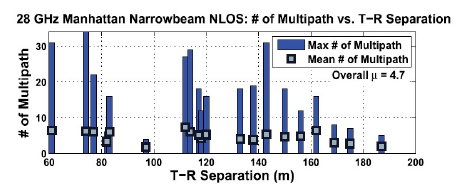
\includegraphics[width=0.8\linewidth]{figs/fig3.2}
    \caption{28 GHz unique antenna azimuth and elevation pointing angle, NLOS
        maximum and mean MPCs as a function of TX-RX separation distance for
        narrow-beam antenna measurements in Manhattan. The overall mean number
        of MPCs over all TX-RX antenna pointing angle combinations and TX-RX
    separation distances is also presented \cite{Rappaport2015}.}
    \label{fig:3.2}
\end{figure}
Basing on the reviewed papers we can conclude that mmWave channel features
allow one to single out several strong propagation paths and determine their
AOAs.

\section{Оценка угла прихода (Angle of arrival estimation)}

Как показано выше, канал миллиметрового диапазона можно представить в виде
набора геометрических лучей.  Самые сильные лучи могут быть
использованы для передачи данных. Как правило, диаграмма направленности
антенны формируется по направлению луча прямой видимости (Line of Sight).
Однако в случае не прямой видимости (Non Line of Sight), может быть
выбран самый сильный отраженный луч. Это причина, почему определение угла
прихода играет ключевую роль в некоторых случаях формирования ДН. Оценка угла
прихода,которая также упоминается в литературе как оценка угла места,
обычно рассматриваемая в задачах радиолокации. Для этих задач уже
разработаны алгоритмы и аппаратные реализации во времена зарождения радиолокации. Эти
алгоритмы совершенствовались, с появлением фазированных антенных решеток.
Этот опыт кажется чрезмерно полезным при наличие аппаратных ограничений систем
связи миллиметрового диапазона при низком количество цифровых портов по сравнению с имеющимся
количеством антенных элементов.  Другой набор алгоритмов пришел из приложений
спектрального анализа. В них обычно предполагается, что сигнал каждой антенны
принимается независимо.  Эти алгоритмы очень эффективны и дают возможность
оценить направления на несколько целей (лучей) одновременно и имеют
сверхразрешение способность. С другой стороны, они
требуют значительных вычислительных ресурсов.
Кроме того, есть некоторые дополнительные специальные методы, такие как
synthesizing a virual aperture, позволяет достигать высокого разрешения и
точности пеленгации. 
В этом разделе мы рассмотрим и систематизируем существующие подходы
к оценке АОА, которые нам удалось найти в открытых литературных источниках.
Будут представлены их преимущества и недостатки.  
На этапе моделирования в следующей части этой работы, мы сократим этот список и
выделим наиболее перспективные методы.

\subsection{Метод Фурье и метод средних периодограмм}

Простейшая алгоритм оценки AOA называется бимформинг \cite{Tuncer2009, Stoica2005}. В
некоторой литературе этот метод также называется метод Фурье \cite{Allen2006}. 
Основная идея заключается в максимизации мощности, принятой с определенного
направления.

Определим сигнал $\vec{y}(t)$ принятой антенной решеткой от некоторого
удаленного источника.

\begin{equation}
    \label{eq:3.1}
    \vec{y}(t) = a(t) \vec{s}(\phi_{src}) + \vec{\xi}(t),
\end{equation}
где ${\vec{s}(\phi_{src})}$ весовой вектор источника сигнала,
$\phi_{src}$ -- угол прихода (AOA); $\vec \xi$ -- вектор шума.
A certain elevent of the steering vector is 
Каждый элемент весового вектора представляется в виде
\begin{equation}
    \qty{\vec{s}(\phi)}_n = \exp{-i(\vec k (\phi), \vec \rho_n)},
\end{equation}
где $\vec k (\phi_{src})$ is n-ый волновой вектор, $\vec\rho_n$ радиус-вектор
n-го элемента антенны. 
В случае эквидистантной антенной решетки (ULA), последнее уравнение приведется
к виде
\begin{equation}
    \qty{\vec s(\phi)}_n = \exp{i2\pi\frac{d}{\lambda}\sin(\phi)n},
\end{equation}
где $d$ -- расстояние между элементами антенной решетки, $\lambda$ -- длина
волны излученного сигнала.

Чтобы получить максимальную мощность с какого-то направления
$\phi$ необходимо сформировать соответствующую диаграмму направленности
(бимформинг). Это делается с использованием так называемого вектора бимформинга
$\vec w (\phi) = \vec s(\phi)/\rVert(\vec s(\phi))\lVert$.

На практике, этот весовой вектор обычно модифицируется окном, выбранным
для подавления уровня боковых лепестков ДН до необходимого уровня. Мы будем
использовать нормированный, но не взвешенный вектор бимформинга, что делает
мощность шума на выходе формирователя луча (принимаемую мощность) такой же, как
на антенне.

Here we use a normalized but nonwindowed weight vector,
which makes the noise power at the beamformer output (received power) the same as at the antenna
elements \cite{Tuncer2009}. 

На основе вектора бимформинга искомая функция будет следующей
\begin{equation}
    p(\phi) = \abs{\vec w^H (\phi) \vec y}^2.
\end{equation}

Физически, функция $p(\phi)$  является мощностью выходного сигнала антенной
решетки. Тогда оценка АОА получается как значение угла
$\phi$, обеспечивающий максимум функции $p(\phi)$.

\begin{equation}
    \phi = argmax~p(\phi)
\end{equation}

\begin{figure}
    \centering
    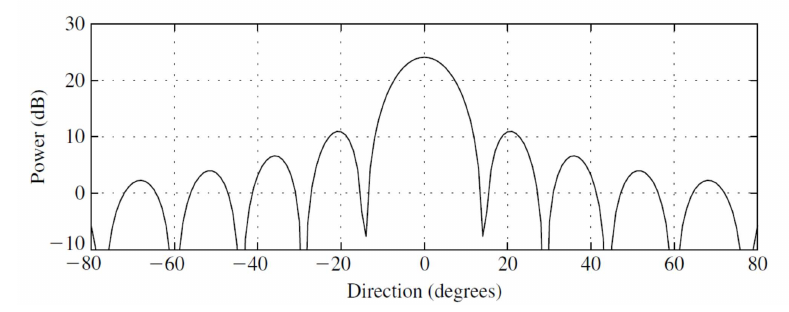
\includegraphics[width=\linewidth]{figs/fig3.9}
    \caption{ДН (невзвещенная) для 16-ти элементной эквидистантной линейной
        решетки ($\frac{d}{\lambda}=0.5$), сформированной на направление 0
        град. \cite{Tuncer2009}. }
    \label{fig:3.9}
\end{figure}

Отметим, что этот алгоритм соответствует обобщенной оценке максимального
правдоподобия в случае модели \eqref{eq:3.1} \cite{Tuncer2009}.

Для фазированной антенной решетки
функция поиска может быть оценена во временной области посредством переключения
луча. Если количество приемников (цифровых портов) равно количеству антенных
элементов, искомая функция $p(\phi)$ может быть оценена в цифровой области \cite{Stoica2005}.
В литературе этот подход также называется методом Бартлетта \cite{Godara2004}. 

Функция $p(\phi)$ примет вид
\begin{equation}
    p(\phi) = \frac{\vec s^H(\varphi) \hat{\vec M} \vec s (\phi)}{N^2},
\end{equation}
где $\hat \vec M$ -- оценка корреляционной матрицы принятого сигнала
\begin{equation}
    \hat {\vec M} = \frac{1}{L} \sum\limits_{t=1}^{L} \vec y(t) y^H (t)
\end{equation}

%As for sidelobe level, it can affect AOA estimation in case of multipath propagation. In order to
%reduce sidelobe level antenna array is weighted with some window function which sets amplitude
%spatial distribution. There are plenty of window functions. The most common of them are Hamming,
%Hanning, Bartlett, Blackman, Chebyshev and Kaiser windows. Note that choice of the window is
%always a trade-off between side lobes level (interference influence) and main lobe width (resolution).
%For example, the Blackman window provides the lowest side lobes level and the widest main lobe.
%Unlike other windows which are fixed, Kaiser and Chebyshev windows provide some flexibility in
%resulting beam pattern properties. The Kaiser window is an approximation of the
%optimal window which maximizes the relative energy in the main lobe
%\cite{Stoica2005}. 
%It is often chosen over the fixed window
%designs because it has a lower sidelobe level when it is selected to have the same main lobe width as
%the corresponding fixed window (or narrower main lobe width for a given sidelobe level). The
%Chebyshev window has the property that the peak level of the sidelobe “ripples” is set constant.
%Under this restriction the window provides the minimal main lobe width. The detailed windows
%description and their comparison analysis can be found in \cite{Stoica2005}
%\cite{Allen2006}. Note, that listed window
%functions can be implemented in hardware via fixed attenuation in waveguides.
%The beamforming based DOA estimation algorithm can be implemented relaying on beam sweep
%procedure used in mm wave communication systems for beam management \cite{Chavva2019}.
%Finally, we can distinguish the following pros and cons of this approach.
Что касается уровня боковых лепестков, то он может повлиять на оценку AOA при многолучевом распространении. Чтобы уменьшить уровень боковых
лепестков антенная решетка взвешивается с некоторой оконной функцией, которая
устанавливает пространственное распределение амплитуды. 
Наиболее распространены окна Хэмминга, Ханнинга, Бартлетта, Блэкмана,
Чебышева и Кайзера. Обратите внимание, что выбор окна всегда компромисс между
уровнем боковых лепестков (влияние помех) и шириной главного лепестка
(разрешение).  Например, окно Блэкмана обеспечивает самый низкий уровень
боковых лепестков и самый широкий главный лепесток.  В отличие от других
фиксированных окон, окна Кайзера и Чебышева обеспечивают некоторую гибкость в
настройке результирующих свойств диаграммы направленности. Окно Кайзера
является аппроксимацией оптимального окна, которое максимизирует относительную
мощность в главном лепестке \cite{Stoica2005}.  Его часто выбирают вместо
фиксированного окна, потому что оно имеет более низкий уровень
боковых лепестков, когда он выбран, чтобы иметь ту же ширину основного
лепестка, что и соответствующее фиксированное окно (или более узкая ширина
основного лепестка для данного уровня бокового лепестка).  Окно Чебышева имеет
то свойство, что пиковый уровень боковых лепестков задается
постоянным.  При этом ограничении окно обеспечивает минимальную ширину главного
лепестка. Подробное описание различных оконных функций и их сравнительный анализ можно найти
в \cite{Stoica2005} \cite{Allen2006}. 
%Обратите внимание, что указанное окно
%функции могут быть реализованы аппаратно через фиксированное затухание в
%волноводах.  Алгоритм оценки DOA на основе формирования луча может быть
%реализован с ретрансляцией по развертке луча.  процедура, используемая в
%системах связи миллиметрового диапазона для управления лучом \cite{Chavva2019}.
%Наконец, можно выделить следующие плюсы и минусы этого подхода.

\paragraph{Преимущества}%
\begin{enumerate}
    \item Теоретически, метод Фурье и метод Бартлетта являются оптимальными
        решениями для оценки AOA в
    случай однолучевого канала.
\end{enumerate}

\paragraph{Недостатки}%

\begin{enumerate}
    %\item In practice, the search accuracy is affected by some adverse factors.
        %First, the derivative of the search function is equal to zero at the
        %extremum point. It leads to “flat” top and makes it difficult to
        %estimate extremum point precisely. Second, it is necessary to provide a
        %high angle discretization rate to provide acceptable AOA estimation
        %accuracy if no additional techniques are used.

    %\item The solution may be not appropriate in case of user mobility if the
        %search is implemented via beam sweeping in time domain.
    %\item The method provides low resolution ability which depends on beam
        %pattern’s main lobe
    %width. Increasing of SNR or evaluation time does not lead to enhancement of resolution
    %quality. That makes this approach hardly matched for multipath AOA estimation.
    %\item In case of close multipath AOA estimation there is significant bias of
        %direction (systematic error).
\item На практике, точность поиска снижается из-за некоторых факторов.
    Во-первых, производная функции $p(\phi)$ равна нулю в
         точка экстремума. Это приводит к «плоской» вершине и затрудняет точное
         определение точки экстремума. Во-вторых, необходимо обеспечить
         высокую дискретизацию по углу для обеспечения приемлемой оценки.
     \item Решение может не подойти в случае достаточно мобильных пользователей, если
         поиск реализован с помощью сканирования во временной области.
     \item Метод обеспечивает разрешающую способность, зависящую
         от ширина главного лепестка ДН. Увеличение SNR или времени
         сканирования не приводит к качественному улучшению разрешения.  Это делает
         этот подход малопригодным для оценки многолучевого АОА.
     \item В случае нескольких близко расположенных АОА наблюдается
         значительно смещение оценки (систематическая ошибка).
\end{enumerate}


\subsection{Метод максимального правдоподобия}%
\label{sub:metod_maksimal_nogo_pravdopodobiia}
При наличии нескольких путей распространения, оптимальная оценка AOA может быть
получена с помощью максимально правдоподовной оценки (MLE).
 \cite{Tuncer2009}. Соответствующая модель сигнала:
\begin{equation}
    \label{eq:3.8}
    \vec y(t) = \sum\limits_{q=1}^{J} a_q(t)\vec s(\phi_q) + \vec \xi(t),
\end{equation}
где $J$ число путей распространения; $a_q(t)$ -- комплексная амплитуда q-то
луча, $\vec s(\phi_q)$ весовой вектор;  $\phi_q$ -- угол прихода (AOA) q-то
луча и $\xi(t)$ -- вектор белого гауссового шума. 
Для этой модели канала критерий МП может быть записан как критерий минимума
среднеквадратичной ошибки (MMSE)
 \begin{equation}
    \label{eq:}
    d(\phi_1, \hdots, \phi_J) = \sum\limits_{t}^{} \abs{\vec(t) -
    \sum\limits_{q=1}^{J} a_q(t) \vec s(\phi_q)}^2 \to_{\phi_q} min
\end{equation}
Это уравнение может быть представлено в виде
\begin{equation}
    \label{eq:}
    d(\phi_1, \hdots, \phi_J) = \sum\limits_{t}^{} \vec y^H(t) \vec
P_\perp(\phi_1, \hdots, \phi_J) \vec y(t) \to_{\phi_q} min
\end{equation}

\begin{equation}
    \label{eq:}
    \vec P_\perp(\phi_1, \hdots, \phi_J) = \vec E - \vec S(\vec S^H \vec S)^{-1}
    \vec S^H,
\end{equation}
where $\vec P_\perp$ is a projection matrix and  $\vec S = \qty[\vec s(\phi_1)
\dots \vec s (\phi_J)]$. The minimization of  $d(\phi_1, \hdots, \phi_J)$
needs to be numerical. 
It is generally computationally intensive and require J-dimensional search. In
general a “brute-force” search over a selected grid of values of $(\phi_1,
\hdots, \phi_J)$ is necessary, followed by
interpolation in the neighborhood of the minimum point to compute the final estimate.

\begin{figure}[h]
    \centering
    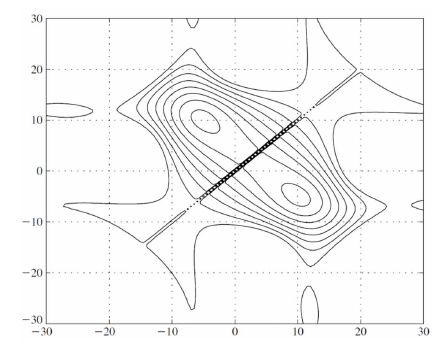
\includegraphics[width=0.6\linewidth]{figs/fig3.10}
    \caption{Maximum likelihood cost function (3.11) for an 8-elemennt ULA and
    two emitters at $\phi_1=-5^\circ$ and  $\phi_2 = 10^\circ$ \cite{Tuncer2009}}
    \label{fig:3.10}
\end{figure}

Finally, we can distinguish the following pros and cons of this approach.
\paragraph{Advantages}%
\label{par:advantages}
\begin{enumerate}
    \item ML estimator provides the optimal solution in case of multiple dominant propagation paths
(AOAs).
\end{enumerate}

\paragraph{Disadvantages}%
\label{par:disadvantages}
\begin{enumerate}
     \item Digital antenna array is required
     \item Excessively high computational cost (“brute force” search).
     \item Maximum likelihood function does not allow one to estimate the number of AOAs. If the
    number of the propagation paths is not known, the method is not optimal.
(AOAs).
\end{enumerate}


\subsection{Monopulse}%
\label{sub:monopulse}

A variation of the beamformer involves a method, often referred to as
monopulse, commonly used in radar systems for target tracking. This method
involves taking the difference between the outputs of two beams pointing in
slightly different directions \cite{Tuncer2009}. The search function is the following
\begin{equation}
    \label{eq:}
    b(\phi) = \frac{1}{\Delta} \qty(\abs{\vec w^H(\phi+0.5 \Delta)\vec y}^2)
    -
    \qty(\abs{\vec w^H(\phi-0.5 \Delta)\vec y}^2) \approx \dv{p(\phi)}{\phi} ,
\end{equation}
where $p(\phi)$ and  $\vec w(\phi)$ are defined as in section 3.2.1. 
The estimation of AOA is obtained as the
value of angle $\phi$ which provides zero search function value
\begin{equation}
    \label{eq:}
    \phi = arg\qty{b(\phi) = 0}.
\end{equation}

In fact, $\Delta$ can be on the order of one beamwidth and $b(\phi)$ will still
be well approximated by derivative of $p(\phi)$ because $b(\phi)$ is nearly
linear over a significant range of angles around the zero- response point
\cite{Tuncer2009}.
This property of the search function gives the opportunity to decrease the
angle discretization rate and apply linear approximation to find AOA. Note,
that this approach is often used together with a rough classical beamforming
method that determines an angle range to accurate search.  An additional
feature of this algorithm is that the output is positive if the emitter is to
the right of the direction in which the difference beam is pointed and negative
if it is to the left. This ability to determine the direction of the emitter
relative to the pointing direction by the sign of the response is useful in
tracking applications \cite{Tuncer2009}.

\begin{figure}[h]
    \centering
    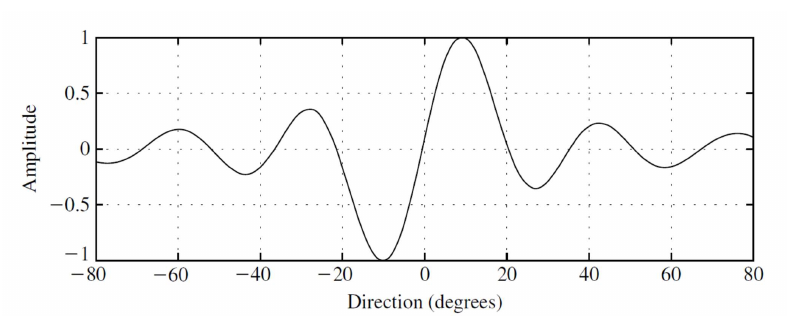
\includegraphics[width=\linewidth]{figs/fig3.11}
    \caption{Response of a monopulse system for 16-element ULA \cite{Tuncer2009}. Source
    direction is 0 deg.}
    \label{fig:3.11}
\end{figure}
Another variant of the algorithm is often called Monopulse Ratio or Amplitude
Comparison Monopulse \cite{Mosca1969}. This algorithm requires coherent reception with two
channels (RF-chains): sum and difference. The sum channel is formed with beam
pattern which has a maximum for a certain direction. The difference beam
pattern has a null for this direction. In \cite{Kim2018} the algorithm which uses TDM for
sum and difference channels is proposed and investigated. It employs cycle
prefix of OFDM signal to receive two identical signals with different beam
patterns using a single RF-chain and phased antenna array. This approach seems
promising, but there are some issues related to phase shifter switching delay
and multipath propagation influence.
The metric of monopulse ratio is \cite{Kim2018}
\begin{equation}
    \label{eq:}
    \tan(\frac{N}{4}(\phi_{src} - \phi)) = 
    \frac{Im\qty{\sum\limits_{k} y_d(k) y_s^*(k)}}{\sum\limits_{k}
    \abs{y_s(k)}^2},
\end{equation}
where $\phi_{src}$ is actual  AOA;  $\phi$ is roughly estimated AOA via beam
sweeping (it is the direction of the sum beam); N is number of antenna
elements; $y_s(k)$ and  $y_d(k)$ are signals f the sum and difference channels
respectively.
 \begin{equation}
    \label{eq:}
    y_s(t) = a(t) \vec w_s^H \vec s(\phi_{src}) + \vec w_s^H \vec \xi(t)
\end{equation}
 \begin{equation}
    \label{eq:}
    y_d(t) = a(t) \vec w_d^H \vec s(\phi_{src}) + \vec w_d^H \vec \xi(t)
\end{equation}

For a linear antenna array the corresponding beamforming vectors are
\begin{equation}
    \label{eq:}
    \qty{\vec w_s (\phi)}_n = \exp{i_2\pi \frac{d}{\lambda}} \sin \phi
\end{equation}
\begin{equation}
    \label{eq:}
    \qty{\vec w_d (\phi)}_{n < \frac n {N}{2}} = - \exp{i_2\pi n \frac{d}{\lambda}} \sin \phi
\end{equation}
\begin{equation}
    \label{eq:}
    \qty{\vec w_d(\phi)}_{n\geq \frac{N}{2}} = +\exp{i2\pi \frac{d}{\lambda}
    \sin \phi (n - 0.5N)},
\end{equation}

\begin{figure}[htpb]
    \centering
    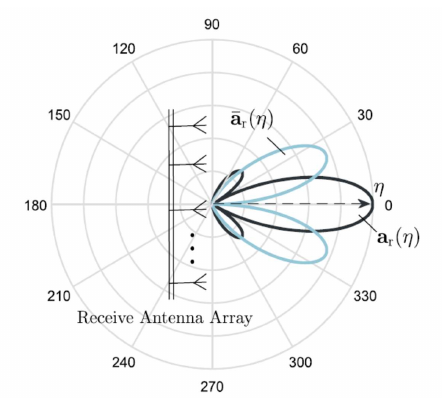
\includegraphics[width=0.6\linewidth]{figs/fig3.12}
    \caption{Sum and difference beam patterns for monopulse ratio algorithm
    \cite{Zhu2016}}
    \label{fig:}
\end{figure}

Monopulse ratio is typically used to estimate a single AOA or resolvable angles
(far spaced targets which are not located within the same beam). However, there
are some modifications that use a complex monopulse ratio and allow one to
detect the multiple targets in a certain beam and estimate their angle
positions \cite{Luoshengbin2016} \cite{Sherman2011}.  As monopulse ratio requires a coherent signal reception
using two channels with different beam patterns it is hardly appropriate for
simple mm-wave system design which consists of only a single RF-chain and can
set only predefined Fourier codebook beams. In \cite{Zhu2016} auxiliary beam approach is
proposed which is similar to monopulse ratio. The principle difference consists
of two points. Firstly, the auxiliary beam approach employs simple beams with a
single main lobe as well as the original monopulse approach does. Secondly, it
employs incoherent signal receptions for different beams and can be implemented
using a single RF-chain.

\begin{equation}
    \label{eq:}
    \zeta_n = \frac{p(\eta_n - \delta) - p(\eta_n + \delta)}{p(\eta_n - \delta)
    + p(\eta_n + \delta)} = 
    \frac{\sin(\psi - \eta_n)\sin\delta}{1 - \cos(\psi - \eta_n)\cos \delta}
\end{equation}

\begin{equation}
    \label{eq:}
    \psi = \eta_n - \arcsin( 
    \zeta_n \frac{\sin\delta}{\sin^2 \delta + \zeta^2_n \cos^2\delta}
    -
    \frac{\zeta_n \sqrt{1-\zeta^2_n} \sin \delta \cos \delta}{\sin^2\delta +
    \zeta^2_n \cos^2 \delta}
    )
\end{equation}
where $\psi_n = 2\pi \frac{d}{\lambda} \sin \phi$ is a spatial frequency for
beam with mainlobe direction angle $\phi$; $\eta$ is a central spatial
frequency for auxiliary beams pair; $n$ is the best auxiliary beams pair index;
$\delta = \frac{\pi}{N}$; $N$ is a number of antenna elements; $p(\eta)$ is
power of received signal for beam with spatial frequency $\eta$.

\begin{figure}[h]
    \centering
    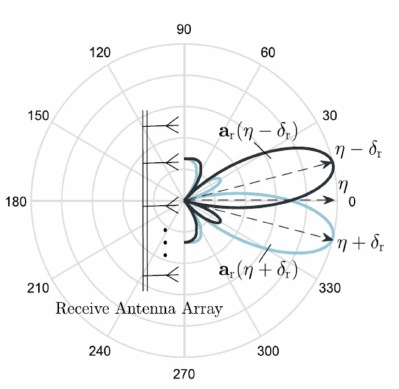
\includegraphics[width=0.6\linewidth]{figs/fig3.13}
    \caption{Auxiliary beam approach patterns \cite{Zhu2016}}
    \label{fig:}
\end{figure}

It is noted in \cite{Sherman2011} that described auxiliary beam approach can provide wrong
result if AOA is near direction of some auxiliary beam and SNR is low, because
it can lead to error in pair selection. In \cite{Sherman2011} it is proposed to employ
additional two beams in this case with the aim to overcome the problem.

\begin{figure}[h]
    \centering
    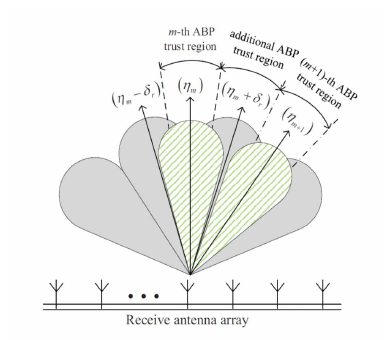
\includegraphics[width=0.6\linewidth]{figs/fig3.14}
    \caption{Auxiliary beam approach and additional auxiliary beam pair
    \cite{Tuncer2009}}
    \label{fig:}
\end{figure}

Finally, we can distinguish the following pros and cons of this approach.
\paragraph{Преимущества}%
\label{par:preimushchestva}

\begin{enumerate}
    \item In practice, it is more convenient and precise than beamforming
        method because the search function is quite steep in the area near AOA.
    \item It can be implemented using phased antenna array with single digital
        port (enable low hardware cost).
    \item Relatively low number of beams is necessary to evaluate AOA.
    \item It potentially could be used together with beam tracking algorithms.
    \item Multiple path AOAs estimation is potentially available using complex
        monopulse ratio.
\end{enumerate}

\paragraph{Недостатки}%
\label{par:nedostatki}
\begin{enumerate}
    \item As a variation of beamforming approach the original method provides
        low resolution ability which depends on beam pattern main lobe width.
        Increasing SNR or evaluation time does not lead to enhancement of
        resolution quality. The high resolution can be achieved using a
        coherent signal reception and complex multipath ratio only.
    \item In case of close multipath AOA estimation, significant bias of
        direction (systematic error) is possible.
\end{enumerate}

\subsection{Minimum variance distortionless response estimator (Capon method)}%
\label{sub:minimum_variance_distortionless_response_estimator_capon_method_}

Another approach similar to beamforming method is Minimum Variance
Distortionless Response Estimator (MVDR) which is also referred to as Capon
method \cite{Stoica2005,Allen2006, Godara2004}. The main idea of this approach is to form beamforming
vector $\vec w(\phi)$  to minimize signal power received from all directions (total
received power) under constant gain for some direction $\phi$.

\begin{figure}[h]
    \centering
    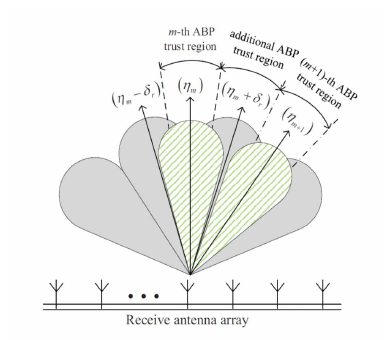
\includegraphics[width=0.6\linewidth]{figs/fig3.14.png}
    \caption{The base idea of Capon method}
    \label{fig:3.15}
\end{figure}
The beamforming vector in this case is obtained as a solution of nonlinear
programming task \cite{Stoica2005, Godara2004}.

\begin{equation}
    \label{eq:}
    \vec w(\phi) = \frac{\hat \vec M^{-1} \vec s (\phi)}{\vec s^H(\phi)\hat
    \vec M^{-1} \vec s(\phi)},
\end{equation}
where $s(\phi)$ is a steering vector defined in (3.2) and $\vec \hat M$ is an estimated signal correlation matrix (3.7).
That leads to the following search function:
\begin{equation}
    \label{eq:}
    p(\phi) = \frac{1}{s^H(\phi) \vec M^{-1} \vec s(\phi)}
\end{equation}
The function represents the received power. The peaks of this function
correspond to AOAs of propagation paths. The resolution of the method increases
with SNR.

For this method we can distinguish the following pros and cons.
\paragraph{Преимущества}%
\label{par:preimushchestva}
\begin{enumerate}
 \item Capon method provides high AOA estimation accuracy.
 \item The method can be used for multiple AOAs evaluation. It provides
     superresolution ability.
 \item It can be implemented in the hardware as the search function has a
     physical meaning of received power.

\end{enumerate}
\paragraph{Недостатки}%
\label{par:nedostatki}

\begin{enumerate}
 \item The resolution is limited even the correlation matrix M is known
     precisely. If one desires to improve the potential resolution, it is
     necessary to increase SNR or the number of antenna elements.
 \item Matrix inversion used in the method has high computational cost.
\end{enumerate}














% % \section{Вторая глава}
% \label{cha:ch_2}

% \subsection{Auxiliary techniques}
% \subsubsection{Synthetic aperture array}

% Antenna movement gives opportunities to apply synthetic aperture for AOA
% estimation \cite{cite37,cite38}. In this case time samples can be presented as
% outputs of some antenna array and any AOA estimation technique can be applied
% for them. In case of uniform linear movement we can write the following
% equation.
% \begin{equation}
%     y(m) = A \exp{2\pi f_0 frac{v}{c} \sin \phi T m},
% \end{equation}
% $A$ -- комплексная амплитуда; 
% $f_0$ -- несущая частота; 
% $v$ -- скорость устройства; 
% $c$  -- скорость света;
% $T$ -- период измерений;
% $\phi$ -- AOA, $m$ -- дискретное время.

% \begin{figure}[ht]
%     \centering
%     \includegraphics[width=0.6\linewidth]{example-image-a}
%     \caption{Антенна с синтезированной апертурой}
%     \label{fig:3.19}
% \end{figure}

% \section{}

\section{Теория}
\subsection{Ограничения и мотивации}
% As the performance of mmWave system depends on beamforming accuracy, the primary task of the
% stage is to develop a precise AOA estimation algorithm. The considered problem has a set of
% significant restrictions which we have taken into account in our research.

Поскольку производительность системы mmWave зависит от точности формирования луча, основная задача
этой работы заключается в разработке точного алгоритма оценки АОА. Рассматриваемая задача имеет множество
существенных ограничения, которые учитываются в этом исследовании.

\begin{enumerate}
    %     \item The AOA estimation algorithm should work using reference signals of NR standard. Thus, it
    % has to use a quite inflexible time structure. Moreover, the algorithm depends on BS’s beam
    % sounding strategy, which is fixed for some reference signals (e.g. a series of DFT-based
    % beams applied by BS during the SS burst).
    \item Алгоритм оценки AOA должен работать на пилотных сигналах стандарта NR. Таким образом, \textit{он
              должен использовать весьма негибкую временную структуру}. Кроме того, алгоритм зависит от луча БС.
          стратегия зондирования, которая фиксируется для некоторых эталонных сигналов (например, ряд основанных на ДПФ
          лучи, применяемые БС во время вспышки СС).
          %     \item SS burst is more preferable reference signal as it does not exploit additional resources.
          % It is desired to use common reference signals for all users, i.e. BS’s cannot use adaptive
          % sounding strategy.
          % User equipment has a single digital port only and beams are formed in analog domain. Thus,
          % some UE’s sounding strategy has to be used.
    \item \textit{SS burst является более предпочтительным эталонным сигналом}, так как он не использует дополнительные ресурсы.

    \item Желательно использовать общие опорные сигналы для всех пользователей, т.е. БС не могут использовать адаптивные
          стратегия звучания.
          Пользовательское оборудование имеет только один цифровой порт, а лучи формируются в аналоговой области. Таким образом,
          необходимо использовать некоторую стратегию звучания УЭ.

    \item Пользовательское оборудование поддерживает формирование диаграммы направленности с помощью фазовращателей. \textit{Нет свободы амплитуды
              степени в векторе формирования луча}.

    \item При переключении луча возникает проблема со скачком фазы. Это значительно
          усложняет когерентный прием для разных лучей и требует некоторого аппаратного решения
          и калибровки. \textit{Таким образом, необходимо сосредоточиться на методах, основанных на мощности, где фаза сигнала
              не измеряется}.

    \item Пользовательская антенная система состоит из \textit{нескольких независимых решеток, которые нельзя использовать
              одновременно}. Каждая решетка покрывает только часть возможных АОА.

    \item Алгоритм должен быть простым.
\end{enumerate}

На основе проведенного обзора литературы (см. \ref{sec:references:review}) мы выделили и разработали
несколько подходов, отвечающих вышеперечисленным требованиям. Первый подход, в качестве базового алгоритма был выбран иерархический поиск (см. \ref{hierarchy:search}).
Это простейший метод, который аппроксимирует алгоритм Фурье (оптимальное решение в случае однолучевого канала) адаптивным дискретным образом.
Основной проблемой этого алгоритма будет ошибка квантования.  В данной работе разработан новый алгоритм, основанный на концепции иерархического поиска. Он использует улучшенную схему измерения и обеспечивает
оценку без ошибки квантования на основе критерия минимума среднеквадратичной ошибки (MMSE).

Второй рассматриваемый алгоритм основан на моноимпульсе, идея которого была предложена в
\cite{Zhu2016, Kim2019}, но только для одной антенной решетки. В данной работе этот алгоритм тестировался и модифицировался под выбранную аппаратную конфигурацию.
Этот алгоритм также обеспечивает непрерывный результат.

Последний рассмотренный алгоритм, так называемый \textit{Adaptive Compressed Sensing Algorithm}, который был предложен в \cite{Alkhateeb2014} для системы HBF (Чё это?)
Этот алгоритм представляет собой схему бинарного поиска со специально разработанной кодовой книгой. Это одно из самых простых и эффективных решений, среди подобных алгоритмов.
Кроме того, он основан исключительно на мощностных характеристиках принятого сигнала.
Однако описанное решение и кодовая книга подойдут только для очень больших антенных решеток
со степенями свободы как по фазе, так и амплитуде. Для выбранной конфигурации, описанное в \cite{Alkhateeb2014} нельзя применить напрямую, поэтому алгоритм пришлось модицицировать.
Основным преимуществом этого алгоритма является сокращение времени зондирования.

Все упомянутые выше улгоритмы были модицицированы для оценки многолучевого AOA.

Далее мы приведем подробное описание алгоритмов, схем измерений и результатов
моделирования.

\subsection{Описание системы и предположения}
\subsubsection{Структура пилотных сигналов}

Стандарт 5G NR включает два типа опорных сигналов, которые можно использовать для обучения луча: SS-burst
и CSI-RS.

SS-burst представляет собой специальный набор опорных сигналов -- блоков синхронизации (SS blocks), предназначенных для
первоначального доступа. Пилотные сигналы занимают полосу в 127. Каждый блок синхронизации
передается с уникальным весовым вектором. То есть только одна пара лучей пользователя и базовой станции может быть прозвонена за один SS блок.
FR2 (mmWave) максимальное количество SS блоков в SS-burst равно 64. SS-burst повторяются с периодом, находящимся  в диапазоне от 5 до 160 мс \cite{Dahlman2018}.
Мы рассматриваем значение по умолчанию 20 мс.

\begin{figure}[h!]
    \centering
    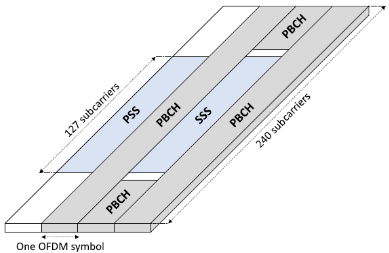
\includegraphics[width=0.4\linewidth]{figs/fig4.1}
    \caption{Структура блока синхронизации}
    \label{fig:4.1}
\end{figure}
\begin{figure}[h!]
    \centering
    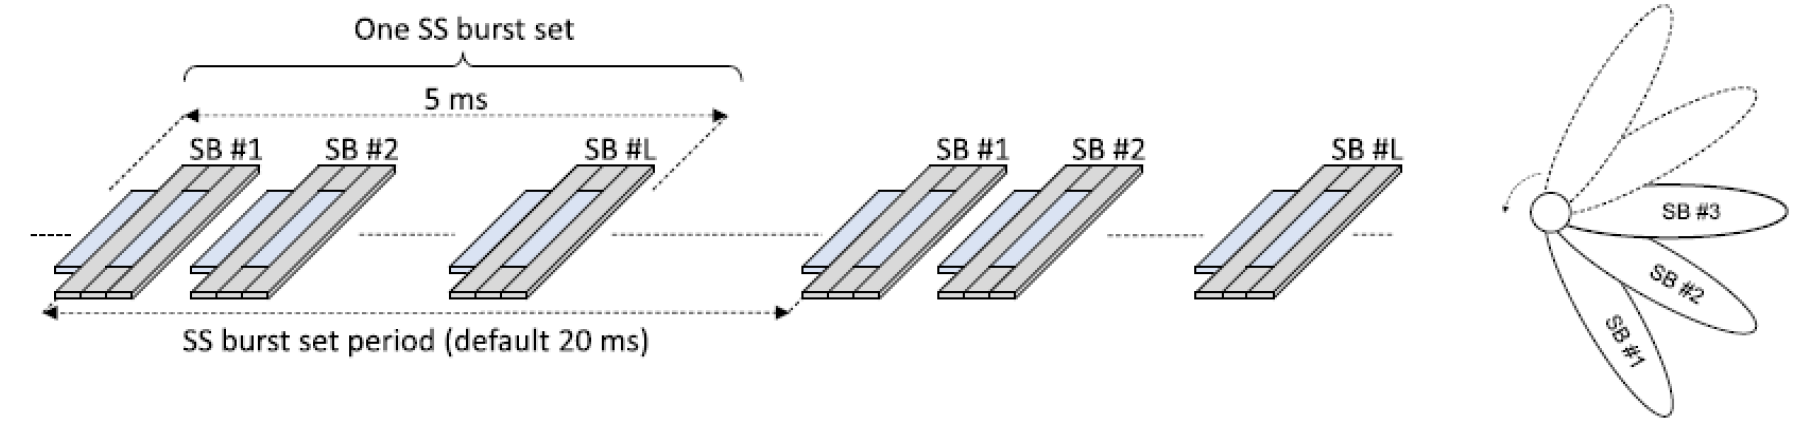
\includegraphics[width=\linewidth]{figs/fig4.2}
    \caption{Последовательность блоков синхронизации (SS-burst)}
    \label{fig:4.2}
\end{figure}

\subsubsection{Пользовательская система антенных решеток}

В данной работе разрабатываются алгоритмы для системы, состоящей из двух линейных эквидистантных антенных решеток, расположенных на противоположных сторонах
устройства (см. \ref{fig:4.3}). В данной конфигурации оборудования, у пользователя нет слепых зон в азимутальной плоскости.

Система содержит только один цифровой порт. Таким образом, решетки не могут
использоваться одновременно и возможно только переключение между ними.

Формирование ДН происходит с помощью непрерывных независимых аналоговых фазовращателями, как показано
на \ref{fig:4.4}.  Диаграмма направленности каждого антенного элемента устанавливается в
соответствии с таблицей 7.3-1 стандарта 3GPP TR 38.901. Ширина луча по уровню -3
дБ составляет $65^\circ$, усиление составляет 8 дБи, ослабление мощности с задней стороны решетки составляет
-30 дБ, поляризация предполагается вертикальной.

\begin{figure}[ht]
    \centering
    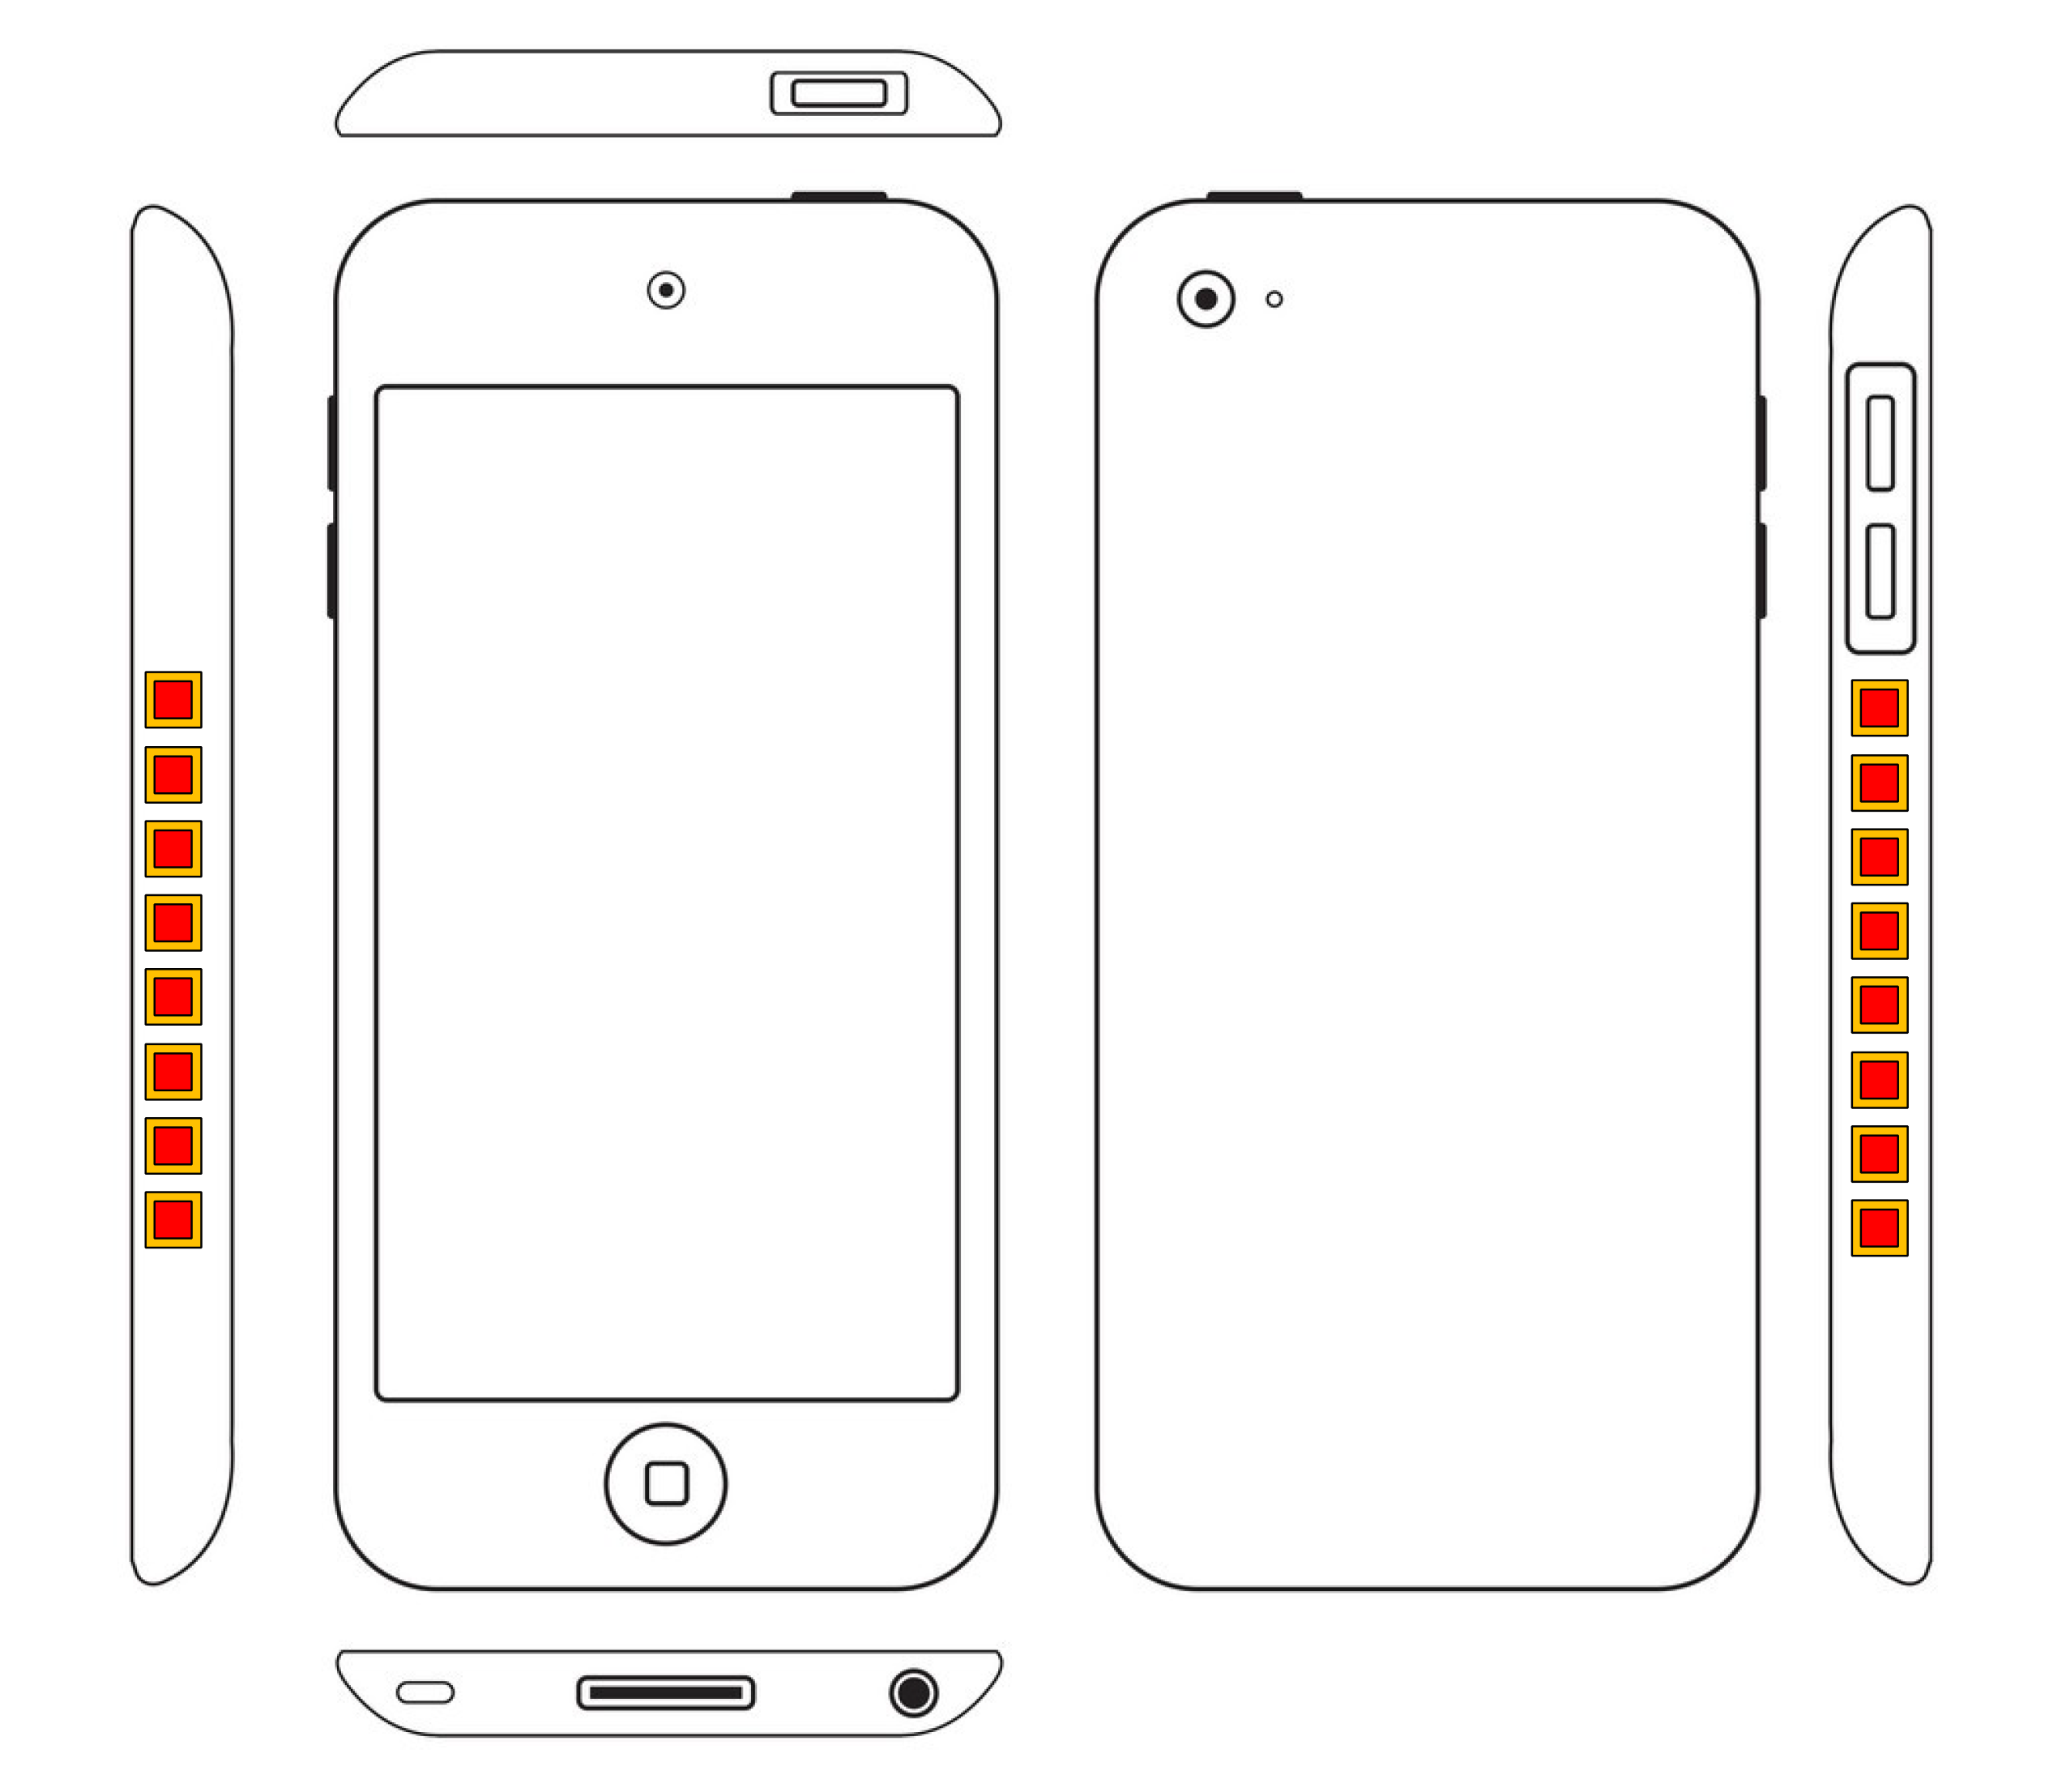
\includegraphics[width=0.5\linewidth]{figs/fig4.3}
    \caption{Расположение антенных решеток на мобильном устройстве}
    \label{fig:4.3}
\end{figure}


\begin{figure}[ht]
    \centering
    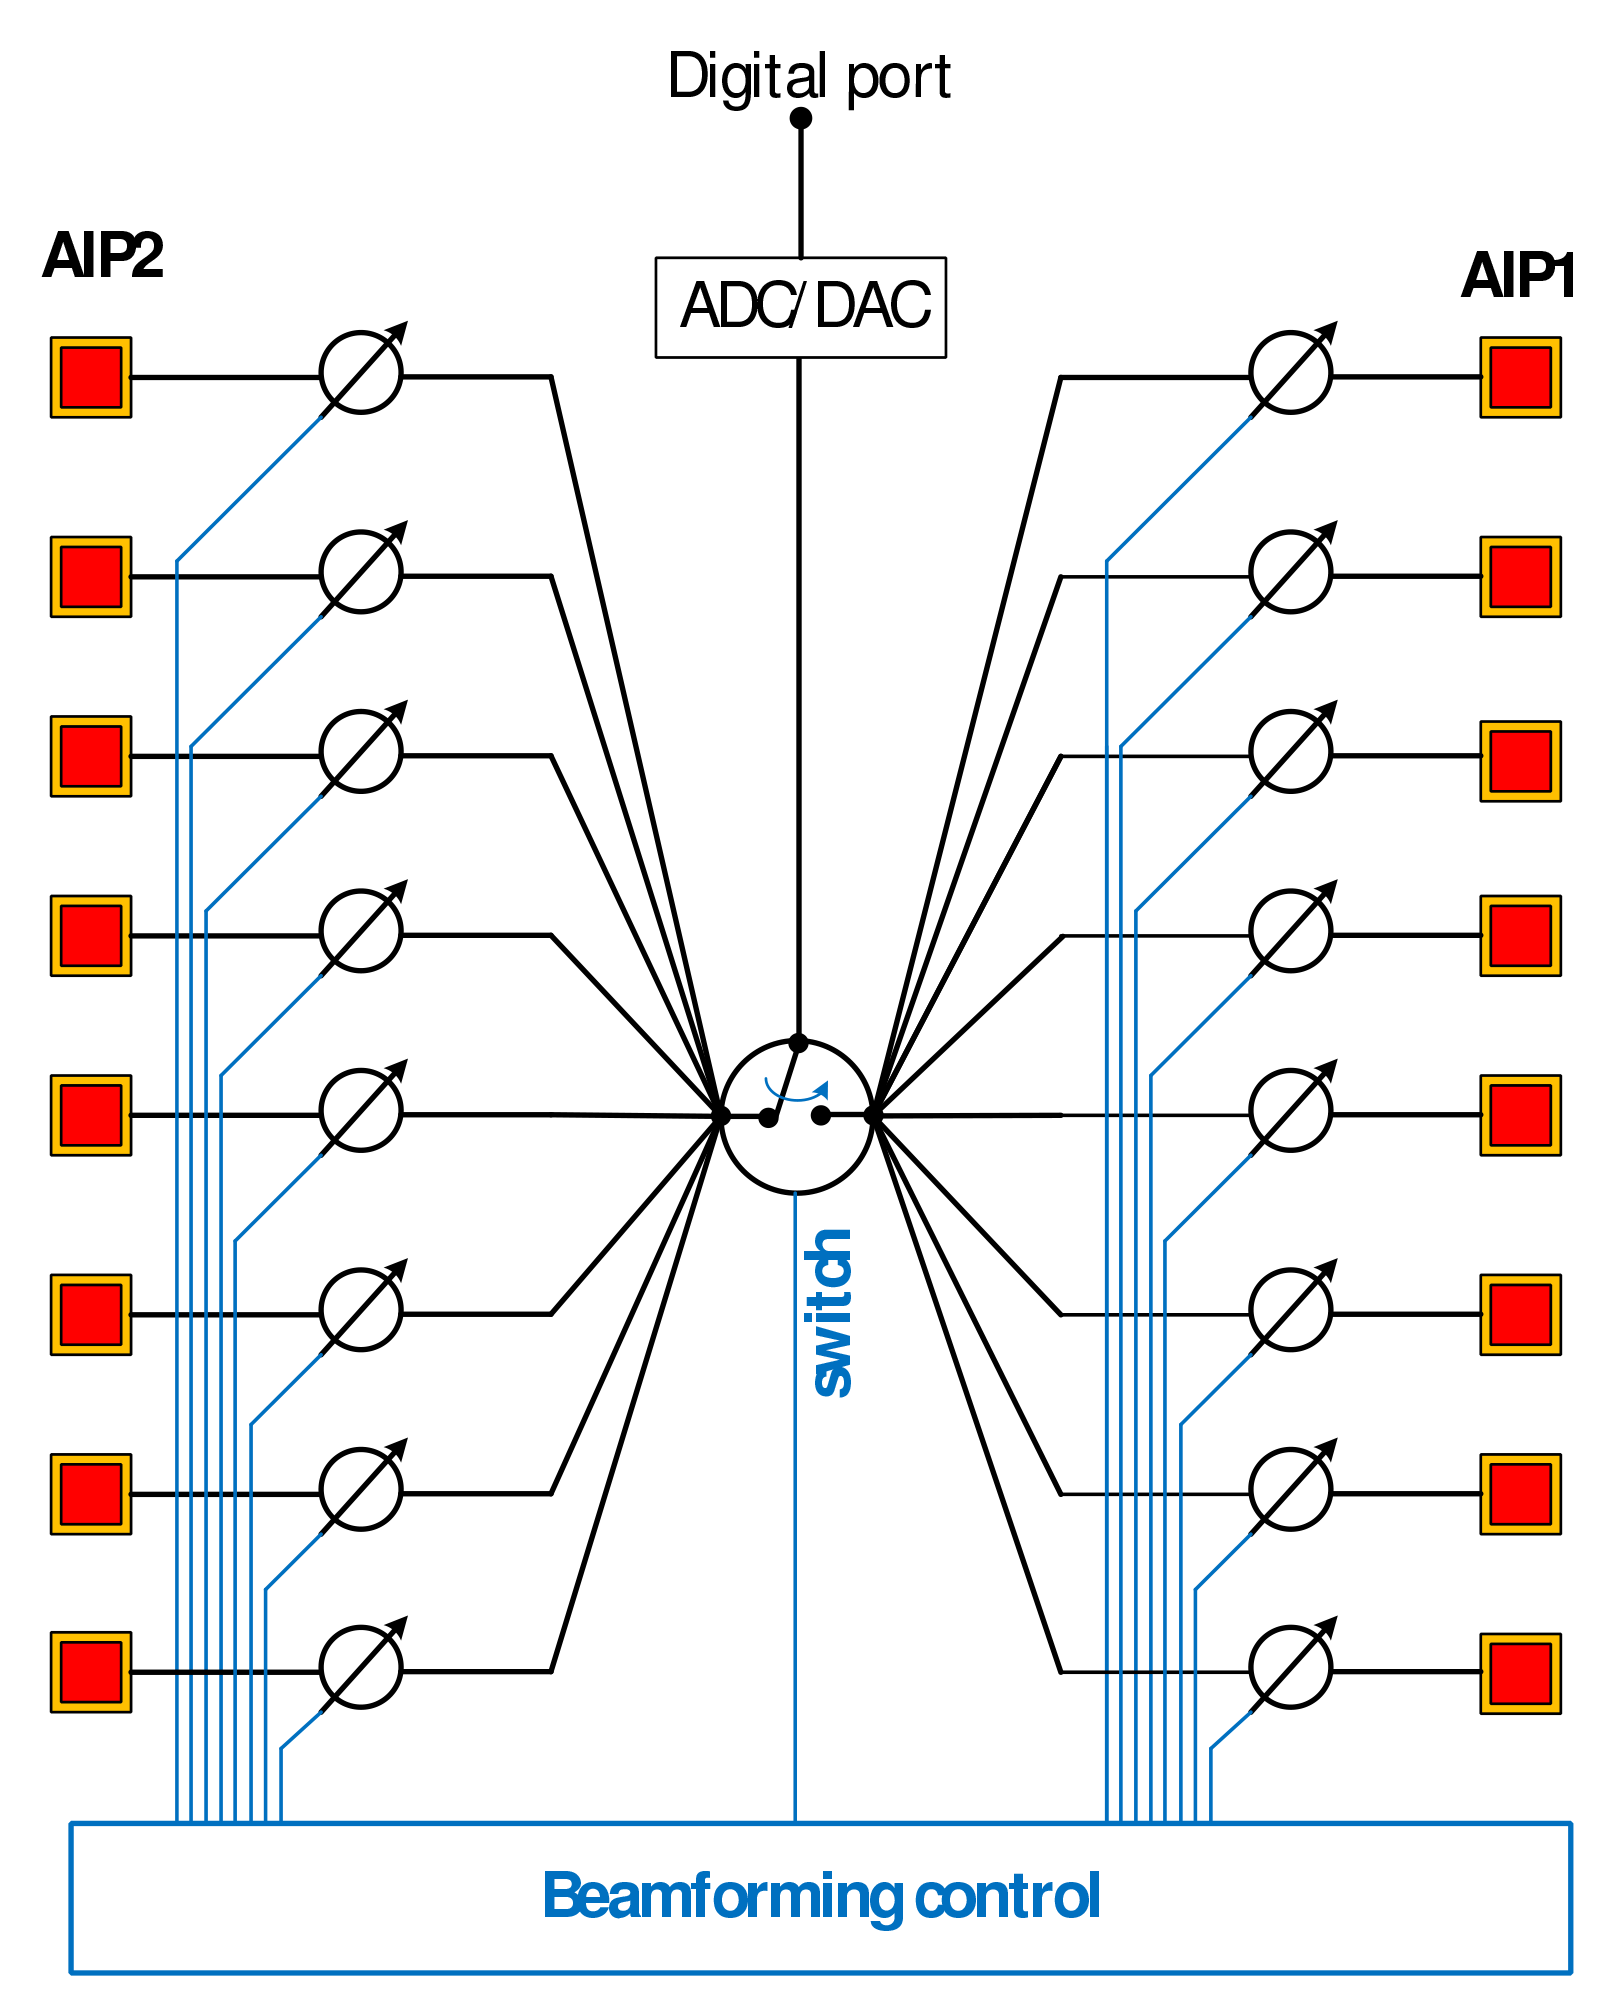
\includegraphics[width=0.4\linewidth]{figs/fig4.4}
    \caption{}
    \label{fig:4.4}
\end{figure}

\begin{figure}[ht]
    \centering
    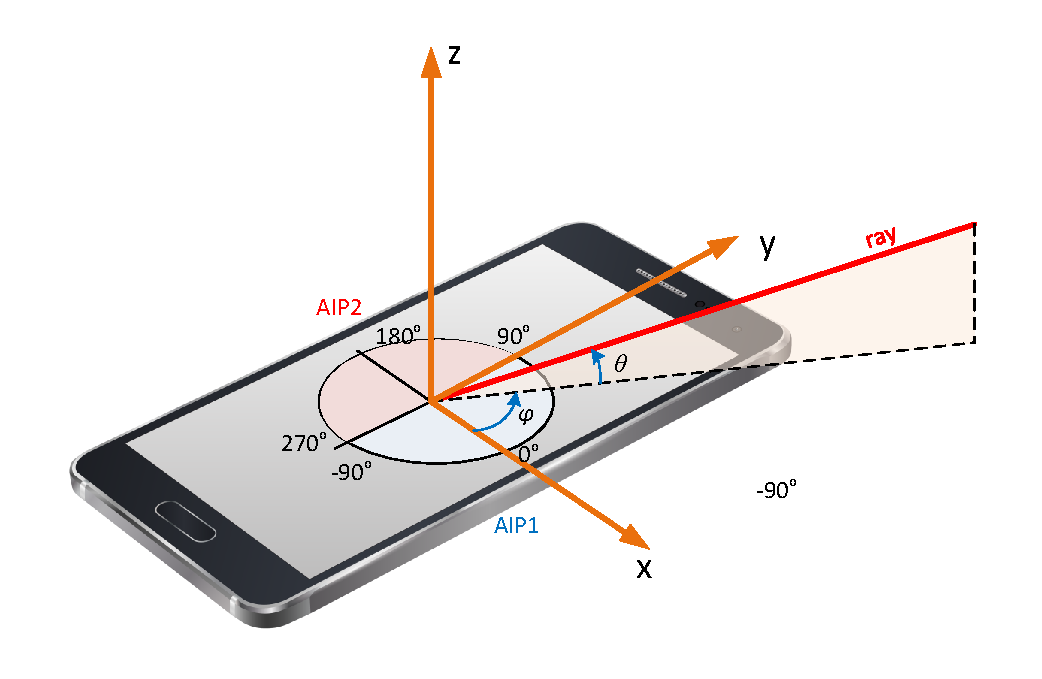
\includegraphics[width=0.75\linewidth]{figs/fig4.5}
    \caption{Локальная система координат пользователя}
    \label{fig:4.4}
\end{figure}


Также стоит определить что мы подразумеваем под угловой координатой источника излучения. Поскольку выбранная антенная решетка линейна, она не может измерять одновременно азимутальный угол и угол места принятого излучения.
Однако, линейная решетка может определить обобщенный угол $\psi$. Тогда мы можем рассматривать некоторый эффективный азимутальный угол $\phi_{eff}$ в качестве угловой координаты источника, который удовлетворяет следующему уравнению
\begin{equation}
    \label{eq:4.1}
    \psi = 2\pi \frac{d}{\lambda} \sin \phi_{eff} = 2\pi \frac{d}{\lambda} \sin\phi \cos{\theta},
\end{equation}
\begin{equation}
    \label{eq:4.2}
    \phi_{eff} = \arcsin(\sin \phi \cos \theta),
\end{equation}
где $\phi$ и $\theta$ -- геометрические углы азимута и элевации источника.

\subsubsection{Антенная решетка базовой станции и система прозвонки}

Антенная решетка базовой станции представляет собой эквидистантную плоскую антенную решетку с 12 строками и 16 столбцами.
Есть два цифровых порта. Формирование диаграммы направленность происходит независимыми непрерывными аналоговыми фазовращателями. Таким образом, можно одновременно
прозвонить два луча, если это позволяет структура пилотного сигнала.

Диаграмма направленности антенного элемента устанавливается в соответствии с
таблицей 7.3-1 стандарта 3GPP TR 38.901. Ширина луча элемента по уровню $-3$ дБ составляет
$65^\circ$. Усиление составляет 8 дБи, ослабление мощности с задней стороны решетки составляет
-30 дБ, поляризация предполагается вертикальной.

В результате, мы имеем 192 пары ортогональных лучей для этой антенный решетки. Однако мы не сможем прозвонить их все за один SS-burst (см. \ref{SS-burst}), поскольку
нам доступно только 64 возможных прозвонки. Для решения этой проблемы учтем два факта.
Во-первых, пользователи в пространстве перемещаются больше в горизонтальной
плоскости, чем в вертикальной. Поэтому можно увеличить ширину луча в
вертикальной плоскости и уменьшить количество лучей с различными углами
элевации.
Во-вторых, в mmWave системе пользователи обычно распологаются ниже БС, поэтому
лучи соответствующие верхнему подпространству БС могут не рассматриваться.

Тогда, проблема решается следующим образом:
\begin{itemize}
    \item Верхние 4 ряда антенной решетки БС отключаются (см. \ref{fig:4.5}), обеспечивая более широкую ДН в вертикальной плоскости
    \item Кодовая книга БС выбирается на основе БФП (см. \ref{codebook}). Горизонтальная сетка обобщенных углов $-\pi + pi/16:\pi/8:\pi-\pi/16$.
          Горизонтальная сетка обобщенных углов $-3\pi/4:\pi/4:0$.
    \item Представленная кодовая книга покрывает нижнюю половину пространства (см. \ref{fig:4.6}), где, как ожидается, будет находиться пользователь.
\end{itemize}

\begin{figure}[ht]
    \centering
    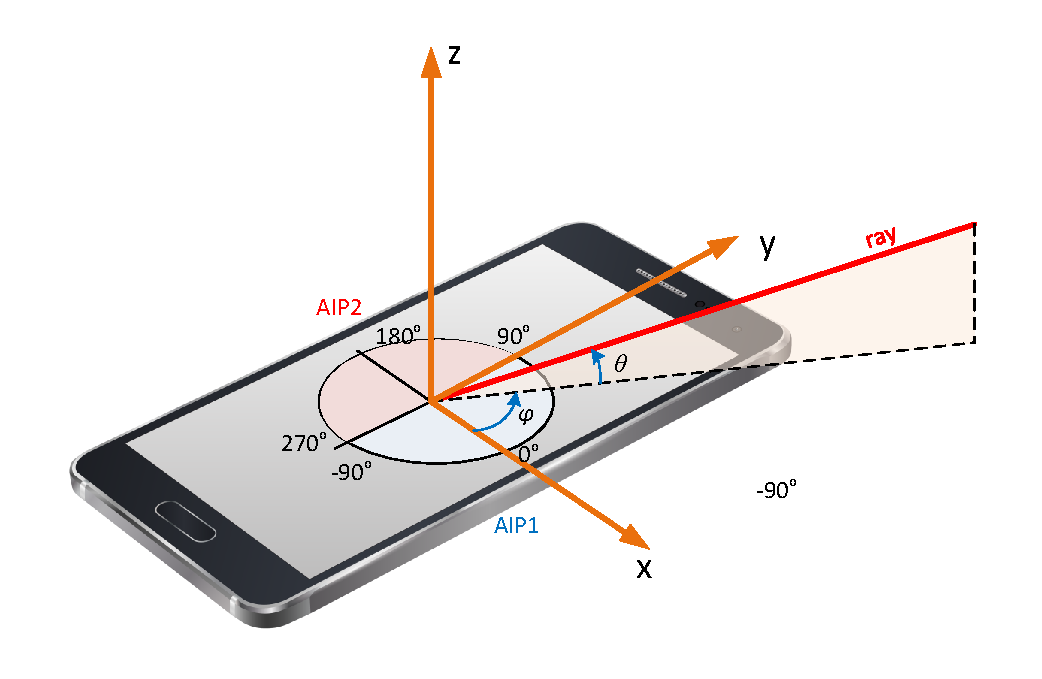
\includegraphics[width=0.35\linewidth]{figs/fig4.5}
    \caption{Серые элементы антенной решетки отключены во время оценки угла прихода}
    \label{fig:4.6}
\end{figure}

\begin{figure}[ht]
    \centering
    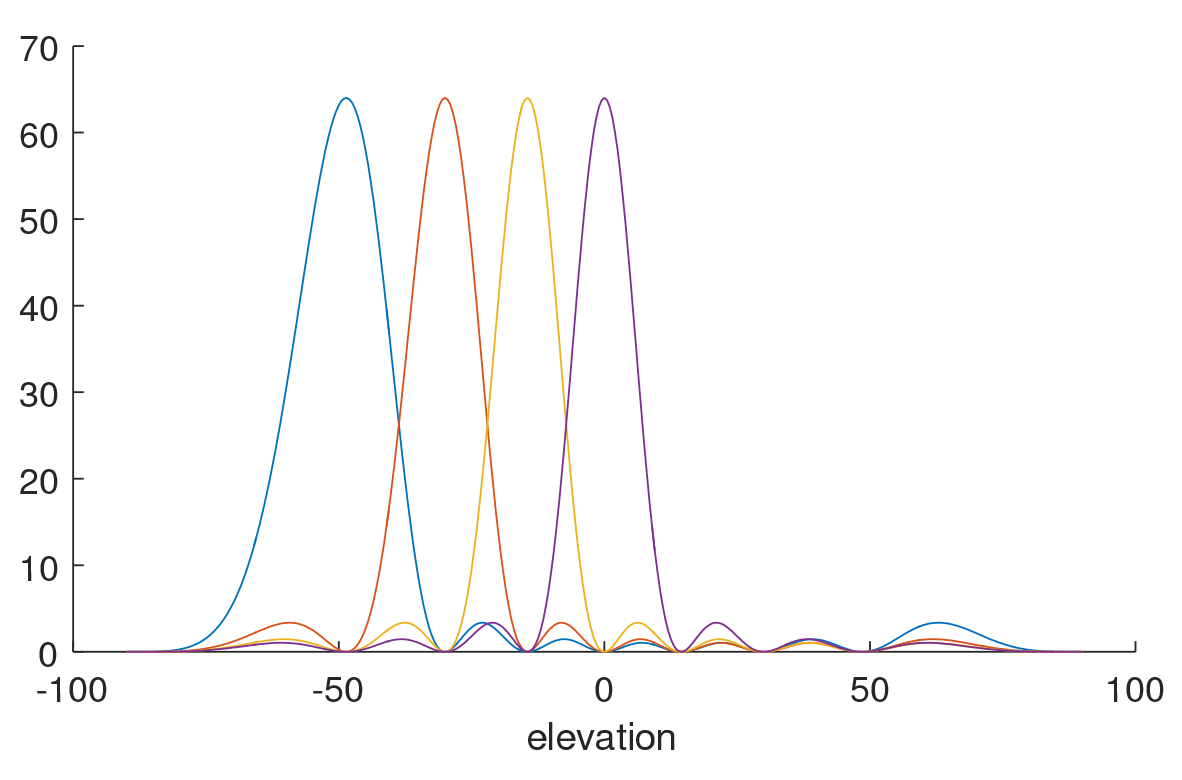
\includegraphics[width=0.5\linewidth]{figs/fig4.6}
    \caption{ДН антенной решетки БС в вертикальной плоскости}
    \label{fig:4.7}
\end{figure}


\subsection{Оценка мощности}
Поскольку разрабатываемые алгоритмы должны быть основаны на мощности, ключевым
моментом является способ измерения мощности сигнала. Для каждой пары лучей UE-BS
у нас есть набор пилотных поднесущих, поэтому у нас есть два пути:
\begin{enumerate}
    \item Усреднить мощность по всем пилотным поднесущим
    \item Использовать Фурье преобразование по всем пилотным поднесущим, перейти от частотной характеристики канала к временной и оценить мощность как максимум импульсной характеристиках канала
\end{enumerate}

Возьмем для начала однолучевую модель канала. В этом случае сигнал, принятый на $q$-ой пилотной поднесущей примет вид
\begin{equation}
    x_q = a e^{-i2\pi q\Delta f \tau} + \xi_q,
\end{equation}
где $a$ амплитуда луча, включающая в себя диаграмму направленность элемента, $\Delta f$ расстояние между пилотными поднесущими в частотной области, $\tau$ -- задержка распространения, $\xi$ -- белый гауссовый шум с мощностью $\sigma^2$.
Для первого варианта, оцененная мощность примет вид
\begin{equation}
    \hat p_1 = \frac{1}{Q} \sum\limits_{q = 0}^{Q - 1} \abs{x_q}^2,
\end{equation}
где $Q$ -- число пилотных поднесущих. После несложных вычислений, можем получить
\begin{equation}
    \mean{\hat p_1} = \abs{a}^2 + \sigma^2.
\end{equation}
\begin{equation}
    D_1 = \mean{p_1^2} - \mean{p_1}^2 = \frac{1}{Q}\qty(2\abs{a}^2 \sigma^2 + \sigma^4),
\end{equation}
где $\mean{\dots}$ -- математическое ожидание, $D$ -- дисперсия оценки мощности.



Во всех алгоритмах нас будет интересовать $\abs{a}^2$ или пропорциональная ей величина.
Относительная систематическая ошибка $\delta_{s1}$ и относительная случайная ошибка $\delta_{r1}$ равны
\begin{equation}
    \delta_{s1} = \frac{\mean{\hat p_1} - \abs{a}^2}{\abs{a}^2} = \frac{\sigma^2}{\abs{a}^2},
\end{equation}
\begin{equation}
    \delta_{r1} = \frac{\sqrt{D_1}}{\abs{a}^2} =
    \frac{1}{\sqrt{Q}} \sqrt{2 \frac{\sigma^2}{\abs{2}} +
        \frac{\sigma^4}{\abs{a}^4}},
\end{equation}

Для второго варианта, оцененная мощность будет вычисляться следующим образом
\begin{equation}
    \hat p^2 = \max_n(\frac{1}{Q} \sum\limits_{q=0}^{Q-1} x_q e^{-2 \pi q n /Q})^2,
\end{equation}
где $n$ -- индекс в оцененной дискретной ИХ канала. Если предположить, что выбор максимума всегда осуществляется корректно, можно получить следующее
\begin{equation}
    \mean{\hat p_2} = \abs{a}^2 F + \frac{1}{Q}\sigma^2.
\end{equation}
\begin{equation}
    D_2 = \mean{\hat p_2^2} - \mean{\hat p_2}^2 = \frac{2\abs{a}^2 F \sigma^2}{Q},
\end{equation}
\begin{equation}
    F = \max_n \frac{\sin^2[\pi Q (\Delta f \tau - n/Q)]}{Q^2 \sin^2[\pi(\Delta f \tau - n/Q)]},
\end{equation}
\begin{equation}
    \frac{4}{\pi^2} \leq \frac{1}{Q^2 \sin^2[\frac{\pi}{2Q}]} \leq F \leq 1,
\end{equation}


Таким образом, мы видим, что оценка мощности также смещена, но систематическая
ошибка меньше, чем в первом случае.
Так как любой постоянный коэффициент $F$ не важен в алгоритмах, а
лишь обеспечивает дополнительный выигрыш во временной области, относительную
систематическую ошибку $\delta_{s2}$ и относительную случайную ошибку $\delta_{r2}$ следует
определять как
\begin{equation}
    \delta_{s2} = \frac{\mean{\hat p_2} - F \abs{a}^2}{F \abs{a}^2} = \frac{1}{Q} \frac{\sigma^2}{F\abs{a}^2},
\end{equation}
\begin{equation}
    \delta_{r2} = \frac{\sqrt{D_1}}{F\abs{a}^2} = \frac{1}{\sqrt Q} \sqrt{\frac{2\sigma^2}{F\abs{a}^2}}.
\end{equation}

Если мы используем только пилотные поднесущие для оценки мощности и $FQ > 1$ (т.е. $Q\geq 3$),
мы можем гарантировать, что $\delta_{s2} \leq \delta{s1}$. Поэтому, второй подход к оценке дает меньшую
систематическую ошибку. Что касается случайной ошибки, мы можем сказать, что $\delta_{r_2} \leq \delta_{r_1}$, если
$\abs{^2}/\sigma^2 < 0.34$ (т.е. SNR на поднесущую составляет -4.7 дБ или меньше).

Таким образом, второй подход к оценке мощности для алгоритма AuxBeam и случаев с
низкими SNR. Также, если задачей является оценка угла на основной луч в
многолучевом канале, второй подход уменьшает помехи, вызванными остальными лучами.
Однако в случае многолучевой оценки угла прихода второй подход приводит к
высокой сложности, поскольку мы должны рассматривать трехмерную задачу для
каждого пути распространения.

Таким образом, в работе применеются следующая схема оценки мощности
\begin{enumerate}
    \item Для оценки угловой координаты в однолучевом канале, мы применяем второй подход (TOA selection) \\
    \item Для оценки угловой координаты в многолучевом канале, мы применяем перывй подход (усреднение принятой мощности по пилотным поднесущим) \\
\end{enumerate}

\section{Однолучевые алгоритмы оценки угла прихода сигнала}
\subsection{Базовый алгоритм}
Эффективность базового алгоритма, также будем называть его \textit{baseline}, рассматривается как нижняя граница разработанных алгоритмов.
Первоначально базовый алгоритм рассматривался нами как полный перебор по всем парам лучей (UE-BS), примененный к эволюционировавшему во времени каналу.
Однако он дает слишком высокую ошибку дискретизации и сравнивать с ним результаты других алгоритмов оказалось не наглядно. Поэтому в дальнейшем в этой работе под базовым алгоритмом будет пониматься
алгоритм иерархического поиска. Алгоритм состоит из двух этапов: полного перебора всех пар лучей UE-BS и процедуры уточнения.
На первом этапе пользователь использует ортогональную кодовую книгу, покрывающую диапазон углов от $-\pi$ до $\pi$:
\begin{equation}
    \vec w_u =
    \begin{bmatrix}
        1 & \exp {i \eta_u} & \dots & \exp{i(N-1)\eta_u}
    \end{bmatrix}^T
\end{equation}
\begin{equation}
    \eta_u = -\pi \frac{N-1}{N} + 2\pi \frac{u-1}{N},
\end{equation}
где $N$ -- число элементов антеннйо решетки, $u$ -- индекс весового вектора, лежащий в интервале $\qty[1 \dots N]$, $\eta_u$ -- обобщенный угол, соответствующий углу прихода сигнала следующим образом
\begin{equation}
    \eta_u = 2\pi \frac{d}{\lambda_w}\sin\phi_u,
\end{equation}
где $d$ -- расстояние между элементами решетки, $\lambda_w$ -- длина волны. ДН,
получаемые с помощью данной кодовой книги показаны на рис. \ref{fig:4.9}
сплошными линиями.
\begin{figure}[ht]
    \centering
    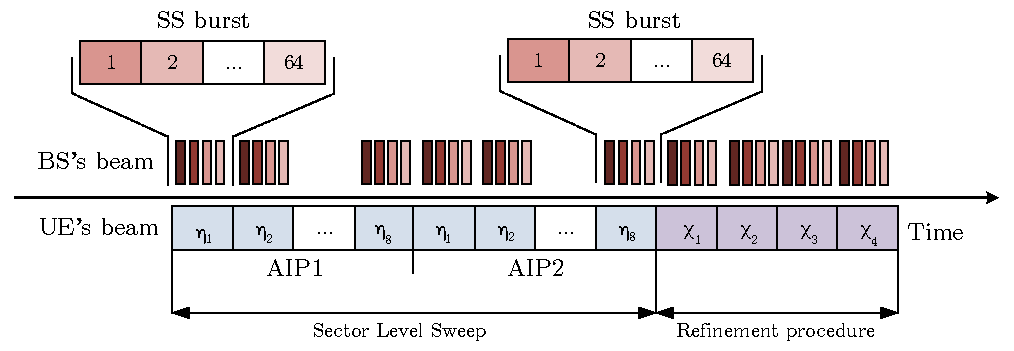
\includegraphics[width=0.5\linewidth]{figs/fig4.9}
    \caption{Различные ДН, формируемые кодовой книгой на стороне пользователя. $\psi$ -- обобщенный угол, $N=8$, $M=4$}
    \label{fig:4.9}
\end{figure}

Пусть $v$ -- индекс наилучшего весового вектора $\vec w_u^{(v)}$, который обеспечивает наибольшую принятую мощность на антенной решетке.
Соответствующая ДН показана на рис. \ref{fig:4.9} толстой спложной линией. Пусть $p_v$ -- мощность, измеренная для вектора $\vec w_u^{(v)}$. На этапе процедуры уточнения
пользователь тестирует $M$ дополнительных весовых векторов, чтобы уменьшить ошибку дискретизации.
\begin{equation}
    \label{eq:4.19}
    \vec w_q =
    \begin{bmatrix}
        1 & \exp {i \chi_q} & \dots & \exp{i(N-1)\chi_q},
    \end{bmatrix}^T
\end{equation}
\begin{equation}
    \chi_q = \eta_v + 2\pi \frac{q}{N(M+1)},
\end{equation}
где $q=-0.5M,\dots,-1,+1,\dots,+0.5M$. Сформированные дополнительные ДН показаны на рис.\ref{fig:4.9} пунктирными линиями.

Мы можем положить $p_0= p_v$ и $\chi_0 = \eta_v$. Отметим, что для процедуры уточнения не нужно проводить измерения $\chi_0$, поскольку оно уже было сделано на предыдущем этапе.
Наонец, путь распространения с обобщенным углом $\hat \psi$ оценивается как один из $\chi_q \in \qty{\chi_{-0.5 M}, \dots, \chi_0, \dots, \chi_{+0.5M}}$,
обеспечивающий наибольшую измеренную мощность $p_q$. Угол прихода соответствующего луча оценивается как
\begin{equation}
    \hat \phi = \arcsin{\frac{\psi \lambda_w}{2\pi d}}.
\end{equation}

Процедура измерения алгоритма представлена на рис. \ref{fig:4.10} и происходит следующим образом:
\begin{enumerate}
    \item Sector Level Sweep Stage. BS periodically sweeps its beams. UE
          sequentially uses each beam of codebook (4.16) to measure power for each
          beam of BS. This procedure is performed for AIP1 and AIP2
    \item We choose the best UE-BS beam pair and consider the selected UE’s
          beam as the best sector with spatial frequency $\eta_v$.
    \item Refinement procedure stage. BS periodically sweeps its beams. UE
          sequentially uses each beam of codebook (4.19) to measure power for each
          beam of BS.
    \item We choose the best UE-BS beam pair among all measured at step 3 and
          measured for the central beam of the best sector at step 1. The spatial
          frequency of the selected UE’s beam is $\hat \psi$.
          %  \item If the best UE-BS beam pair is related to AIP1, $\hat \phi_{AOA} = \hat \phi$ 
          %  determined in (4.21).  If the best UE-BS pair is related to AIP2, φ ̂_AOA=φ
          %  ̂+ π. The result is obtained in radians.
\end{enumerate}

\begin{figure}[ht]
    \centering
    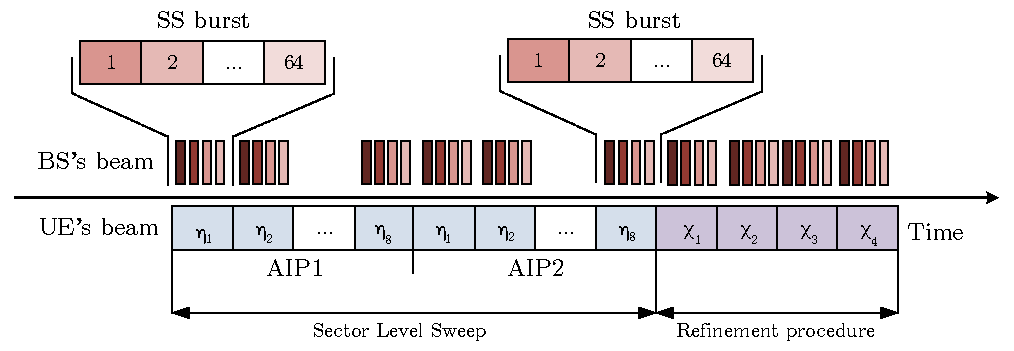
\includegraphics[width=\linewidth]{figs/fig4.9}
    \caption{Изображение процедуры иерархического поиска (baseline) во времени для двух антенных решеток. $N=8$, $M=4$, 64 луча BS}
    \label{fig:4.9}
\end{figure}

Параметры алгоритма иерархического поиска представлены в таблице \ref{tab:4.2}.
Предполагается, что один SS-burst состоит из 64 RS и занимает 32 последовательных слота с периодом 20 мс.

\begin{table}
    \caption{Параметры алгоритма иерархического поиска (baseline)}
    \label{tab:4.2}
\end{table}


\subsection{Иерархический поиск с минимизацией СКО}
В теории оценивания AOA доказано, что наилучшее решение дает максимально правдоподобная оценка (Maximum Likelihood Estimator).
Рассматривая случай однолучевого канала, можно представить уравнение \eqref{eq:3.10} в виде
\begin{equation}
    d(\phi) = \sum\limits_q \vec y^H(q) \vec y(q) - \sum\limits_q\abs{\vec y^H \vec s(\phi)}^2 \to \min_\phi,
\end{equation}
\begin{equation}
    \label{eq:4.23}
    \sum\limits_q \abs{\vec y^H(q) \vec s(\phi)}^2 = \hat p(\phi) \to \max_\phi,
\end{equation}
где $\vec y$ -- вектор принятого антенной решеткой сигнала, $\vec s(\phi)$ --
диаграммобразующий вектор. Выражение \eqref{eq:4.23} имеет смысл мощности,
принимаемой с  вектором $\vec s(\phi)$, обеспечивающим максимум ДН в направлении
$\phi$. Максимизация этого значения есть ни что иное, как непрерывное
сканирование лучом и получение пространственного распределения мощности.

На практике, мы не можем применить этот оптимальный алгоритм по нескольким
причинам. Во-первых, мы управляем лучами дискретными фазовращателями и можем
оценить только дискретный спектр мощности. Разумеется, можно применить некоторые
методы интерполяции, но это будет только приближение.  Во-вторых, у нас есть
сильные ограничения по времени, особенно в случае динамического канала.  Таким
образом, метод иерархического поиска, который адаптивно измеряет дискретный
спектр мощности, представляется наиболее подходящей аппроксимацией оптимального
ML-оценки.  Однако, приближение спектра мощности с помощью иерархического
поиска, каким он рассматривался в предыдущем разделе \eqref{sec:hierarchy}, не
является удачной аппроксимацией.  Прежде всего потому что это приближение с
ошибкой дискретизации. К тому же, если искомая угловая координата источника
лежит на стыке  двух антенных решеток $\hat \phi \approx \pm \pi$ или же просто
при низком SNR,  можно ошибиться с выбором антенной решетки и эта ошибка не
будет исправлена в дальнейшем. С учетом этим недостатков, был разработан
улучшенный алгоритм иерархического поиска.

На первый взгляд, проблема дискретизации может быть решена с помощью
ML-оценки, адаптированного к последовательному измерению отклика мощности
луча. Однако полученная в этом случае функция правдоподобия сложна для анализа
(здесь предполагается, что амплитуда принимаемого сигнала имеет распределение
Райса).

\begin{equation}
    F_{ML}(\psi, a) = \prod\limits_m \frac{1}{\sigma^2}
    \exp{-\frac{\hat p_m + a f_m(\psi)}{\sigma^2}
        I_0\qty(\frac{2\sqrt{\hat p_m a f_m(\psi)}}{\sigma^2})} \to \max_{\psi, a},
\end{equation}
где $\hat p_m$ -- измеренная мощность на $m$-ом луче, $\sigma^2$ -- мощность
шума, $a$ -- "мощность" некоторого путя распространения, $I_0(x)$ --
модицицированная функция Бесселя, $f_m(\psi)$ -- усиление АР для $m$-го луча в
направлении обобщенного угла $\chi_m$, $\psi = 2\pi \frac{d}{\lambda_w}\sin
    \phi$ -- обобщенный угол, а $\phi$ -- угол прихода.
\begin{equation}
    f_m(\psi) = \frac{\sin^2 (0.5N(\psi - \chi_m))}{\sin^2(0.5(\psi - \chi_m))}.
\end{equation}
Поскольку мы пытаемся найти простое решение, мы предлагаем взять в основу критерий минимума СКО, вместо ML-оценки.
\begin{equation}
    \label{eq:26}
    F_{MMSE}(\psi, a) = \sum\limits_m \qty(\hat p_m - a f_m(\psi))^2 \to \min_{\psi,a}
\end{equation}

В первую очередь, необходимо исключить параметр $a$ из уравнения \eqref{eq:26}.
\begin{equation}
    \pdv{a} F_{MMSE}(\psi, a) = \sum\limits_m 2f_m(\psi) (\hat p_m - a f_m(\psi)) = 0
\end{equation}
\begin{equation}
    a(\psi) = \qty[\sum\limits_m f_m(\psi) \hat p_m][\sum\limits_m f_m^2(\psi)]^{-1}.
\end{equation}
Тогда, окончательный результат
\begin{equation}
    F_{MMSE}(\psi)=\underbrace{\sum\limits_m \hat p_m^2}_{\const} - \qty[\sum\limits_m f_m(\psi) \hat p_m]^2 \qty[\sum \limits_m f_m^2 (\psi)]^{-1} \to \max_{\psi}
\end{equation}
\begin{equation}
    \label{eq:4.30}
    F(\psi)=\qty[\sum\limits_m f_m(\psi) \hat p_m]^2 \qty[\sum \limits_m f_m^2 (\psi)]^{-1} \to \max_{\psi}
\end{equation}
На рис. \ref{fig:4.10} представлен вид функции \eqref{eq:4.30} во время процедуры уточнения для точной оценки угла прихода.

\begin{figure}[htbp]
    \begin{subfigure}{0.49\linewidth}
        \centering
        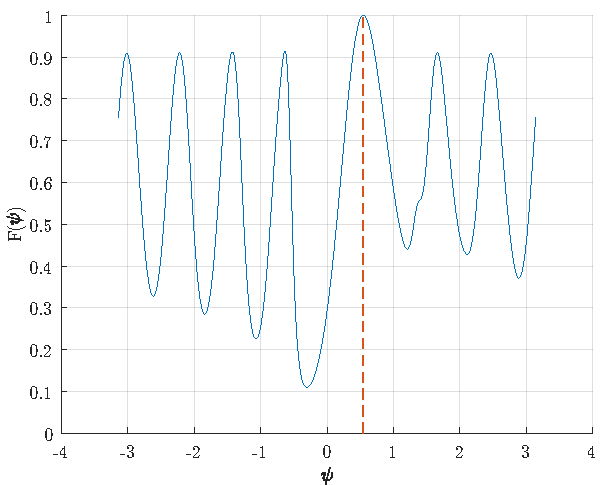
\includegraphics[width=\linewidth]{figs/fig4.10a}
        \caption{}
        \label{fig:4.10a}
    \end{subfigure}
    \begin{subfigure}{0.49\linewidth}
        \centering
        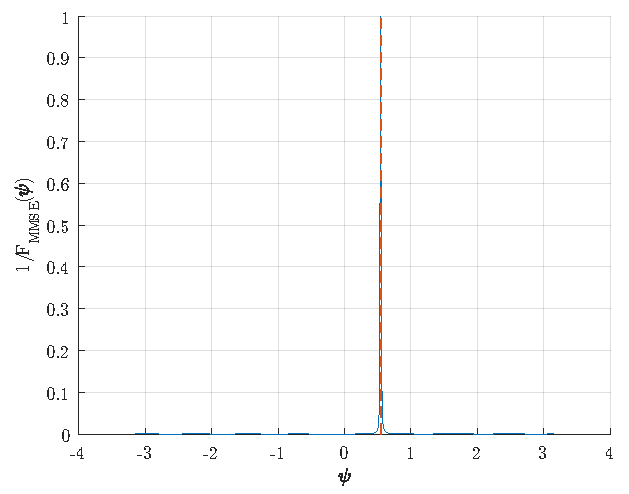
\includegraphics[width=\linewidth]{figs/fig4.10b}
        \caption{}
        \label{fig:4.10b}
    \end{subfigure}
    \caption{ \subref{fig:4.11a} Инверсная нормированная $F_{MMSE}(\psi)$, \subref{fig:4.11b} нормированная $F(\psi)$, $\psi=10^\circ(\psi \approx 0.55), \text{SNR}=30$ дБ}
\end{figure}

Прямое вычисление $F(\psi)$ и поиск его максимума ведет к большим вычислительным затратам. Можно применить условие $F'(\psi) =0$ и получить следующее условие
\begin{equation}
    \label{eq:4.31}
    \begin{aligned}
        \mu(\psi) = &
        \qty(\sum\limits_m f'_m(\psi) \hat p_m) \qty(\sum\limits_m f^2_m(\psi))                              \\
                    & - \qty(\sum\limits_m f_m(\psi)\hat p_m) \qty(\sum\limits_m f_m (\psi) f'_m(\psi)) = 0,
    \end{aligned}
\end{equation}
\begin{equation}
    \label{eq:4.32}
    \begin{aligned}
        f'_m(\psi) = \frac{\sin(0.5N (\psi - \chi_m))}{2\sin^3(0.5(\psi - \chi_m))} \times
        \big[
          & (N-1)\sin(0.5(N+1) (\psi - \chi_m)) - \\
        - & (N+1) \sin(0.5(N-1)(\psi - \chi_m))
            \big]
    \end{aligned}
\end{equation}
Некоторый график $\mu(\psi)$ представлен на рис. \ref{fig:4.11}. Можно заметить, что вокруг заданного $\psi \approx 0.55$ (красная вертикальная линия) есть область где
$\mu(\psi)$ положительна слева и отрицательна справа. Поэтому, если известна грубая оценка угла прихода (что и происходит при иерархическом поиске), мы можем методом дихотомии быстро найти AOA с машинной точностью.
\begin{figure}[ht]
    \centering
    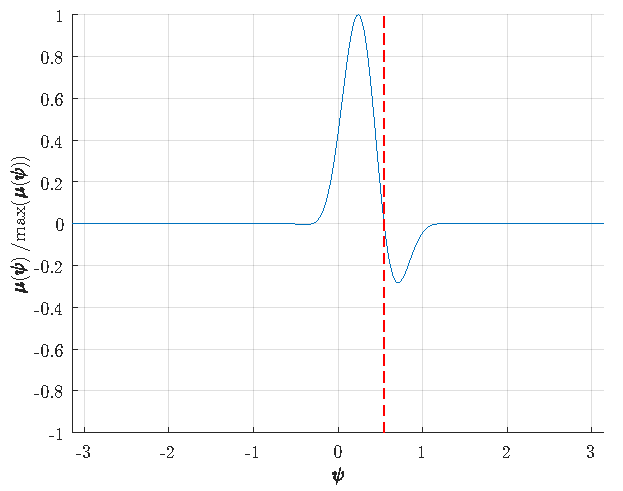
\includegraphics[width=0.75\linewidth]{figs/fig4.11}
    \caption{Нормированная функции $\mu(\psi)$, $\psi=10^{\circ} (\psi \approx 0.55), SNR=30$ дБ}
    \label{fig:4.12}
\end{figure}

\begin{algorithm}
    \caption{Метод дихотомии для оценки угла прихода для улучшенного алгоритма иерархического поиска (hSearchMMSE)}
    \label{lst:4.1}
    \begin{algorithmic}
        \State $\psi_{left} = \psi_{min}$
        \State $\psi_{right} = \psi_{max}$
        \State $\psi_{old} = \psi_{min}$
        \State $\Delta \psi = \infty$
        \While{$\Delta \psi > \epsilon$}
        \State $\hat \psi = 0.5 (\psi_{left} + \psi_{right})$
        \If{$\mu(\psi) < 0$}
        \State $\psi_{right} = \hat\psi$
        \Else
        \State $\psi_{left} = \hat\psi$
        \EndIf
        \State $\Delta \psi = \abs{\hat \psi - \psi_{old}}$
        \EndWhile
        \State \Return $0.5(\psi_{left} + \psi_{right})$
    \end{algorithmic}
\end{algorithm}

Заметим, что лучи вокруг фактического направления АОА вносят основной
вклад в \eqref{eq:4.30}, потому что они имеют более высокие веса. Таким образом, мы можем
рассматривать только лучи, измеренные на этапе процедуры уточнения, и лучший
луч, выбранный на этапе развертки на уровне секторов. Кроме того, для процедуры
поиска желательно, чтобы фактический угол атаки находился в середине
рассматриваемых направлений лучей. Таким образом, мы должны модифицировать
процедуру измерения на этапе уточнения. Некоторые примеры представлены на рис.
\ref{fig:4.12}.
Сплошными серыми линиями показаны ДН лучей, формируемые на первом этапе оценки.
(развертки на уровне секторов). Сплошная красная линия — диаграмма лучшего луча,
выбранного на первой стадии. Штриховые линии — ДН лучей на этапе
уточнения. Наконец, лучи, используемые в \eqref{eq:4.31}, отмечены цветными кривыми.

Всего, мы имеем два случая. В первом случае фактический угол прихода лежит
вблизи лучшего луча и мы проводим дополнительные измерения вокруг этого луча.
Во втором случае фактический угол прихода лежит посередине между лучшим и соседним
лучами. Следовательно, нам необходимо провести дополнительные измерения между ними.
В этом случае весовые векторы  \eqref{eq:4.19} и \eqref{eq:4.33}.
\begin{figure}[ht]
    \centering
    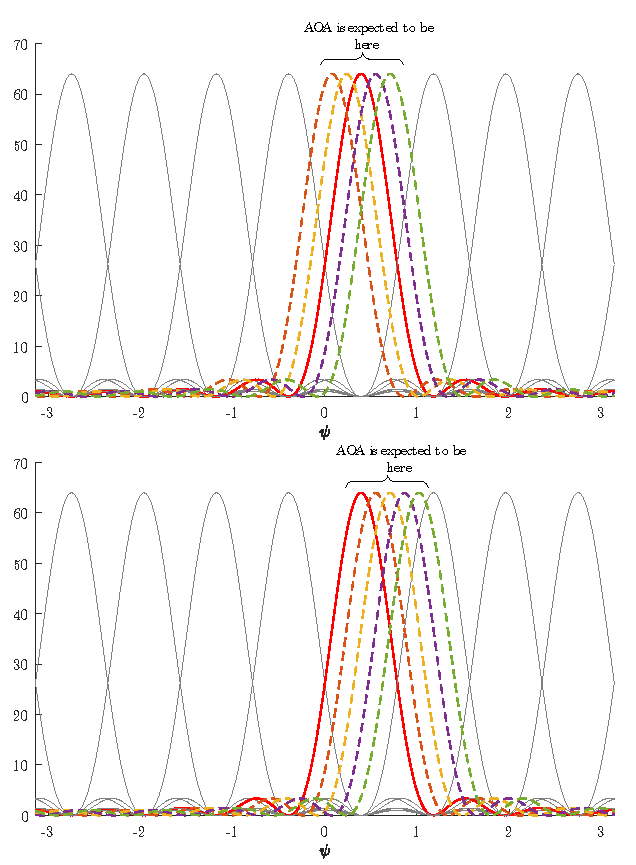
\includegraphics{figs/fig4.12}
    \caption{}
    \label{fig:4.12}
\end{figure}

\begin{equation}
    \label{eq:4.33}
    \chi_q = \eta_v \pm 2\pi \frac{q}{N(M+1)}; ~ q = 1 \dots M.
\end{equation}
Знак зависит от положения лучшего соседнего луча (слева или справа).

Вопрос в том, как мы можем определить, где находится фактический угол прихода до этапа дополнительных измерений.
Предлагается использовать метрику \eqref{eq:4.30} для проверки трех гипотез:
\begin{itemize}
    \item $H_1$ -- угол прихода находится между лучшим лучем и левым соседним лучом
    \item $H_2$ -- угол прихода находится вблизи лучшего луча
    \item $H_3$ -- угол прихода находится между лучшим лучем и правым соседним лучом
\end{itemize}

\begin{figure}[ht]
    \centering
    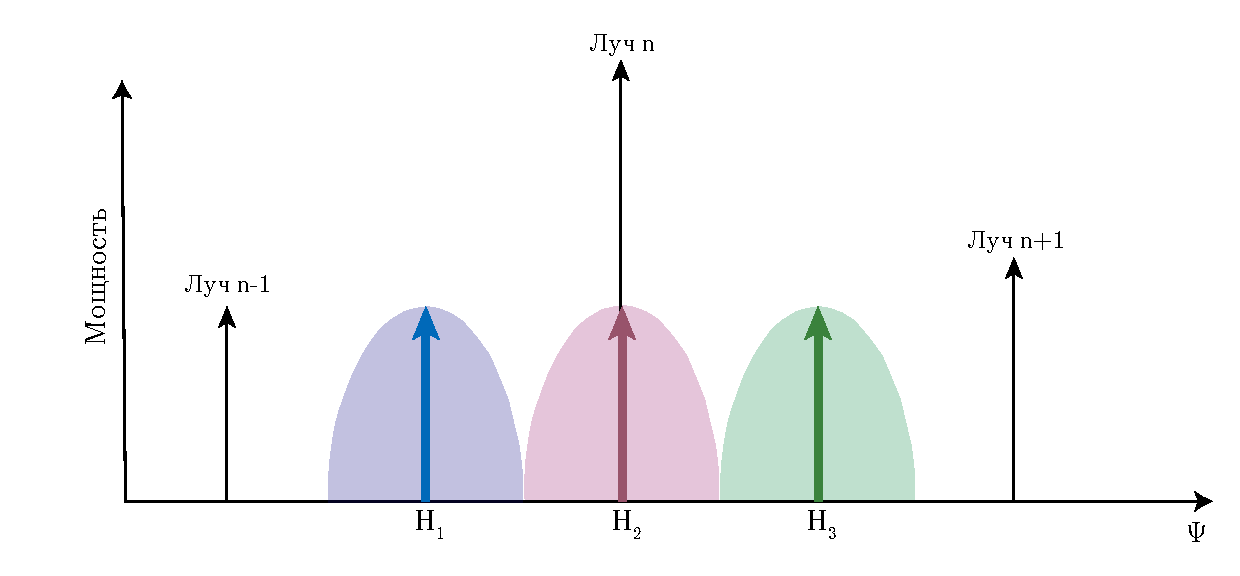
\includegraphics[width=0.75\linewidth]{figs/fig4.13}
    \caption{Выбор гипотез перед дополнительными измерениями. Черные стрелки принадлежат лучам из первой стадии прозвонки, цветные стрелки показываю центральные направления для различных гипотез}
    \label{fig:4.13}
\end{figure}

Если $\eta_v$ --  пространственная частота наилучшего луча на этапе основных измерений, выбранная нами метрика будет равна
\begin{equation}
    \label{eq:4.34}
    F_{H_n} = \qty[\sum\limits_{m=v-1}^{v+1} f_m (\psi_{H_n}) \hat p_m]^2 \qty[\sum\limits_{m=v-1}^{v+1}f_m^2(\psi_{H_n})]^{-1}
\end{equation}
\begin{equation}
    \label{eq:4.35}
    f_m(\psi_{H_n}) = \frac{\sin^2 (0.5N(\psi_{H_n} - \eta_{m}))}{\sin^2(0.5(\psi_{H_n} - \eta_{m}))}.
\end{equation}
\begin{equation}
    \label{eq:4.36}
    \begin{matrix}
        \psi_{H_1} = \frac{\eta_{v-1} + \eta_v}{2}; &
        \psi_{H_2} = \eta_{v}                       &
        \psi_{H_1} = \frac{\eta_{v+1} + \eta_v}{2}; &
    \end{matrix}
\end{equation}


\begin{enumerate}[label=\textbf{Шаг \arabic*:}]
    \item Этап сканирования. BS производит сканирование лучом, UE
          последовательно использует все лучи из кодовой книги \eqref{eq:4.16} для
          измерения мощности на каждом луче BS. Процедура выполняется для обоих AIP.
    \item \label{enum:hSearchMMSE:2} Выбирается лучшая пара лучей UE-BS и рассматривается выбранный луч UE как лучший сектор
          с пространственной частотой $\eta_v$.
    \item Проверяются гипотезы $H_1, H_2$ и $H_3$ (см. \ref{fig:4.13}) используя метрику \eqref{4:34}.
          Выбирается гипотеза с наибольшим значением метрики. Отметим, что в качестве лучшего луча выбирается первый луч UE ($v=1$), то гипотеза $H_1$ не тестируется.
          Аналогично, не тестируется гипотеза $H_3$ для последнего луча с индексом $v=8$.
    \item \label{enum:hSearchMMSE:4} Этап дополнительных измерений. BS также производит сканирование лучом.
          UE последовательно использует все лучи из кодовой книги \eqref{eq:4.19} для
          измерения мощности на каждом луче BS. Если выбрана гипотеза $H_2$, для формирования кодовой книги используется \eqref{eq:4.20}.
          В остальных случаях используется \eqref{eq:4.33}. Знак <<$-$>> соответствует $H_1$, а <<$+$>> соответствует  $H_3$.
    \item Выполняется алгоритм поиска Алг. \ref{lst:4.1}, используя условие МСКО \eqref{eq:4.31}. В уравнение подставляется мощность лучшего луча, измеренная
          на шаге 2 и мощность лучей из шага 4. Луч BS выбирается таким же, как в лучшей паре на шаге 2.
    \item Рассчитывается угол прихода $\hat \phi$ на основе предполагаемой пространственной частоты. Если лучшая пара лучей UE-BS
          относится к AIP1, то $\hat \phi_{AOA} = \hat \phi$. Если лучшая пара UE-BS относится к AIP2, то $\hat \phi_{AOA} = \hat \phi + \pi$.
\end{enumerate}


Временн\'{а}я структура алгоритма hSearchMMSE представлена на рис. \ref{fig:4.9}. Параметры алгоритма представлены в таб. \ref{tab:4.3}.
\begin{table}
    \centering
    \caption{Параметры алгоритма hSearchMMSE}
    \label{tab:4.3}
    \begin{tabular}{|l|c|}
        \hline
        Параметр                             & SS burst  \\
        \hline
        N / M / AIPs                         & 8 / 4 / 2 \\
        Число просканированных лучей (UE/BS) & 20 / 64   \\
        Суммарное число RS                   & 1280      \\
        Необходимое время (слот 0.125 мс)    & 384 мс    \\
        \hline
    \end{tabular}
\end{table}

\subsection{Алгоритм Auxiliary Beam}
Идея алгоритма доп. луча (Auxiliary Beam) была предложена в \cite{Zhu2016} и \cite{Kim2019}. В отличие от
обычных алгоритмов монопульса (см. раздел \ref{sec:3.2.3}), AuxBeam основан на
мощности и не требует сложного измерения амплитуды. Кроме того, для зондирования
требуется достаточно малое количество лучей, и он совместим с алгоритмами
слежения. Таким образом, это хороший кандидат для модификаций.

Основная идея в следующем. Пусть $\eta_u$ и $\eta_{u+1}$ — обобщенные углы лучей такие, что
$\eta_u<\psi<\eta_{u+1}$ (см. рис. \ref{fig:4.14}), где $\psi$ — обобщенный угол прихода волны.
Пусть $\eta_{u+1}$ ортогонален $\eta_u$, то есть $\eta_{u+1} = \eta_u + 2\delta$, где $\delta = \pi/N$  и
$\tilde \eta_u = 0.5 (\eta_u + \eta_{u+1})$ -- центральное направление.
\begin{figure}[ht]
    \centering
    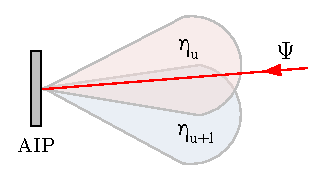
\includegraphics[width=0.5\linewidth]{figs/fig4.14}
    \caption{Конфигурация лучей для AuxBeam}
    \label{fig:4.14}
\end{figure}

Тогда можно рассмотреть следующую метрику, однозначно зависящую от угла прихода
\begin{equation}
    \label{eq:4.37}
    \zeta(\psi) = \frac{f_u(\psi) - f_{u+1}(\psi)}{f_u(\psi) + f_{u+1}(\psi)} = - \frac{\sin(\psi - \tilde \eta_u) \sin \delta}{1 - \cos(\psi - \tilde \eta_u) \cos \delta}
\end{equation}
\begin{equation}
    \label{eq:4.38}
    f_u(\psi) = \frac{\sin^2 (0.5 N (\psi - \eta_u))}{\sin^2(0.5 (\psi - \eta_u))}
\end{equation}
Зависимость метрики $\zeta(\psi)$  от обобщенного угла прихода представлена на
рис. \ref{fig:4.15}.
\begin{figure}[ht]
    \centering
    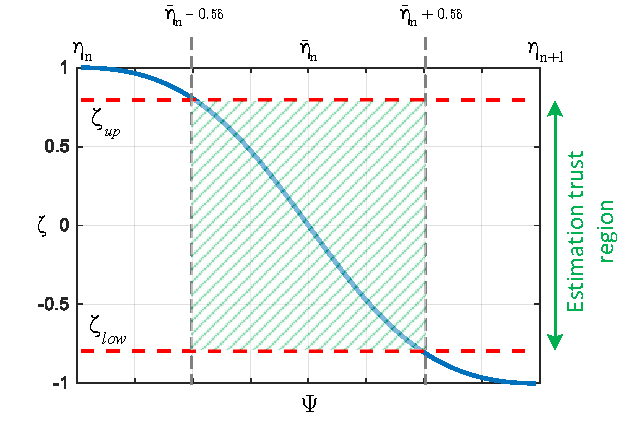
\includegraphics[width=0.5\linewidth]{figs/fig4.15}
    \caption{Зависимость метрики $\zeta(\psi)$ для алгоритма AuxBeam}
    \label{fig:4.15}
\end{figure}
В реальной системе метрика $\hat \zeta$ может быть оценена следующим образом
\begin{equation}
    \label{eq:4.39}
    \hat \zeta = \frac{\hat p_u - \hat p_{u+1}}{ \hat p_u + \hat p_{u+1} },
\end{equation}
где $\hat p_u$ -- мощость измеренная на $u$-ом луче. Эта оценка получается смещенной, поскольку $\hat p_u$ включает мощность шума.
Чтобы избежать этого, в знаменателе можно вычесть удвоенную мощность шума, но это может обратить метрику в бесконечность при малом SNR.
И, поскольку, функция $\zeta(\psi)$ достаточно полога на краях интервала $(\eta_u, \eta_{u+1})$, это приводит к высокому
воздействию шума на метрику при вычислении обратной функции.

Кроме того, если угол прихода находится рядом с центральным направлением определенного
луча, мы можем выбрать другой луч так, что условие $\eta_u<\psi < \eta_{u+1}$ не будет выполняться.
Чтобы этого не произошло, предлагается ввести условие на доверительный интервал
$\zeta_{low}<\hat \zeta < \zeta_{up}$, который изображен зеленой штриховкой  на рис.
\ref{fig:4.15}.

Если условие доверительного интервала не выполняется, следует провести дополнительные измерения на смещенных лучах.
Если оно выполняется, можно оценить угол прихода как
\begin{equation}
    \label{eq:4.41}
    \hat \psi = \tilde \eta_u - \arcsin(
    \frac{\hat \zeta \sin\delta}{\sin^2\delta + \hat \zeta^2 \cos^2\delta} -
    \frac{\hat \zeta \sqrt{1- \hat \zeta^2} \sin\delta\ \cos\delta}{\sin^2\delta + \hat \zeta^2 \cos^2\delta}
    )
\end{equation}
\begin{enumerate}[label=\textbf{Шаг \arabic*:}]
    \item Этап сканирования. BS производит сканирование лучом, UE
          последовательно использует все лучи из кодовой книги \eqref{eq:4.16} и \eqref{eq:4.17} для
          измерения мощности на каждом луче BS. Процедура выполняется для обоих AIP.
    \item По результатам измерений, выбирается лучшая пара лучей UE-BS. Для того же луча BS,
          выбирается самый сильный сосед, первого найденного луча. Используя измеренную мощность для выбранных лучей
          вычисляется метрика \eqref{eq:4.39}. Пример выбранных лучей UE представлен на рис. \ref{eq:4.16}.
    \item Если условие $\zeta_{low} < \hat \zeta < \zeta_{up}$, выполняется оценка обобщенного угла прихода $\hat \psi$ используя \eqref{eq:4.41} и пропускается шаг 4.
    \item Пусть $\eta_v$ -- обобщенный угол лучшего луча UE. Проводятся измерения на обобщенных углах
          $\eta_{v+0.5} = \eta_v - \delta$ и
          $\eta_{v-0.5} = \eta_v + \delta$. Дополнительные лучи показаны на рис. \ref{fig:4.16} пунктирными линиями. Далее вычисляется метрика \eqref{eq:4.39}
          и оценивается обобщенный угол прихода $\hat \psi$ (см. \eqref{eq:4.41}).
    \item Рассчитывается угол прихода $\hat \phi$ на основе предполагаемой пространственной частоты. Если лучшая пара лучей UE-BS
          относится к AIP1, то $\hat \phi_{AOA} = \hat \phi$. Если лучшая пара UE-BS относится к AIP2, то $\hat \phi_{AOA} = \hat \phi + \pi$.
\end{enumerate}

\begin{figure}[ht]
    \centering
    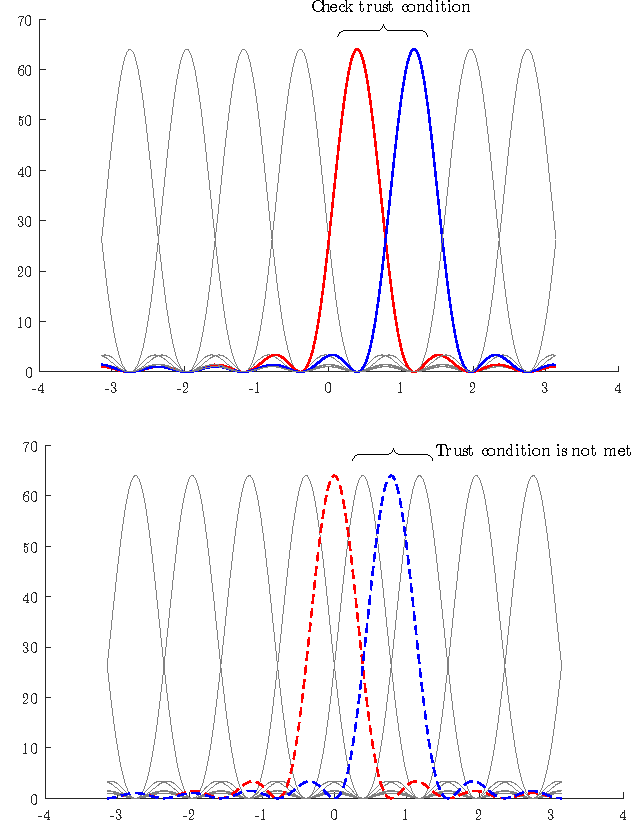
\includegraphics{figs/fig4.16}
    \caption{Два варианта выбора лучей UE для алгоритма AuxBeam. Верхний -- в случае выполнения условия на доверительный интервал, нижний -- в обратном случае.}
    \label{<label>}
\end{figure}


\begin{figure}[ht]
    \centering
    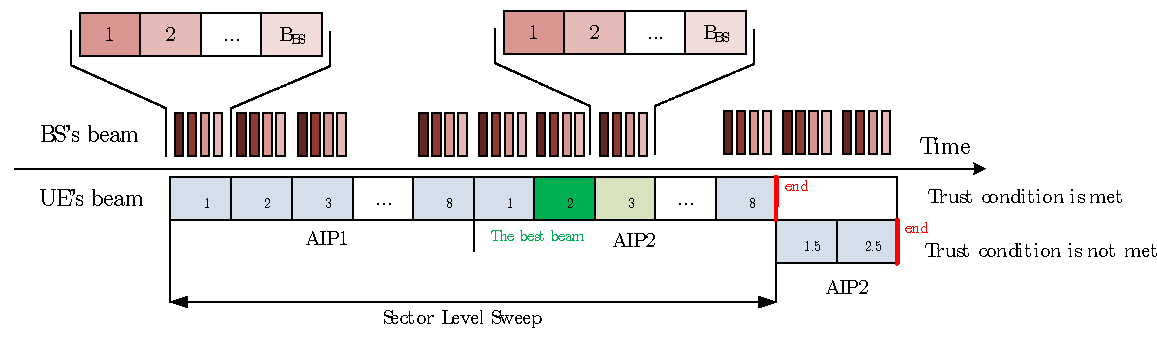
\includegraphics[width=\linewidth]{figs/fig4.17}
    \caption{Изображение процедуры иерархического поиска (baseline) во времени для двух антенных решеток. $N=8$, $M=4$, 64 луча BS}
    \label{fig:4.9}
\end{figure}

Временн\'{а}я структура алгоритма AuxBeam представлена на рис. \ref{fig:4.17}. Параметры алгоритма представлены в таб. \ref{tab:4.4}.
\begin{table}
    \centering
    \caption{Параметры алгоритма AuxBeam}
    \label{tab:4.3}
    \begin{tabular}{|l|c|}
        \hline
        Параметр                             & SS burst        \\
        \hline
        N / M / AIPs                         & 8 / 0 или 2 / 2 \\
        Число просканированных лучей (UE/BS) & 16 или 18 / 64  \\
        Суммарное число RS                   & 1024 или 1152   \\
        Необходимое время (слот 0.125 мс)    & 304 или 344 мс  \\
        \hline
    \end{tabular}
\end{table}

\subsection{Сканирование адаптивным методом бисекций}

Еще один многообещающий метод —  Compressed Sensing Algrorithm, идея которого описана \cite{Alkhateeb2014}.
Базовая концепция следующая. Пусть имеется сетка возможных
обощенных углов прихода волны $\psi_q = - \pi\frac{(Q-1)}{Q} + \frac{2\pi}{Q} (q-1)$, где $Q$ -- размер сетки.
Мы можем представить сигнал, измеренный пользователем (UE) для фиксированного
луча BS, как
\begin{equation}
    \label{eq:4.42}
    y = \vec w^H\vec S \vec a + \vec \xi,
\end{equation}
\begin{equation}
    \label{eq:4.43}
    \vec S =
    \begin{bmatrix}
        \vec s(\psi_1) & \vec s(\psi_2) & \dots & \vec s(\psi_q) \\
    \end{bmatrix},
\end{equation}
\begin{equation}
    \label{eq:4.44}
    \vec s =
    \begin{bmatrix}
        1 & \exp{i\psi} & \dots & \exp\{ i(N-1)\psi\} \\
    \end{bmatrix}^T,
\end{equation}
\begin{equation}
    \label{eq:4.45}
    \vec a =
    \begin{bmatrix}
        0 & \dots & 0 & a & 0 & \dots 0 \\
    \end{bmatrix}^T,
\end{equation}

где $\vec w$ -- весовой вектор пользователя,
$\vec s(\psi)$ -- диаграмообразующий вектор,
$N$ -- число элементов в антенной решетке,
$\vec \xi$ -- вектор шума,
$\vec z$ -- вектор комплексной аплитуды размерности $(Q\times 1)$,
где все элементы нулевые, кроме одного, отвечающему фактическому углу
прихода излучения на решетку.
Основная задача алгоритмов этого семейства -- восстановить вектор $\vec a$
используя количество измерений $L \ll Q$.  Если мы рассмотрим некоторую кодовую
книгу $\vec W$ размером $(N \times L)$, чьи столбцы являются весовыми векторами
для луча пользователя, результат сканирования будет
следующим
\begin{equation}
    \label{eq:4.46}
    y = \vec W^H\vec S \vec a + \vec \xi,
\end{equation}

В работе \cite{Alkhateeb2014}, авторы утверждают, что их адаптивный алгоритм более эфективен,
чем обычный алгоритм бисекции. В адаптивном алгоритме процедура зондирования разбита на несколько этапов
и кодовая книга $\vec W$ текущего этапа зависит от предыдущих результатов. Понятно, что если нас не интересует значение $a$, то
вектор $\vec a$ может быть сжат до вектора $\vec z$. Этот вектор кодирует позицию ненулевого жлемента в векторе $\vec a$ (индекс $q$) и
требует только $\log(Q)$ итераций.

На первом шаге считаем, что ненулевой жлемент имеет индекс от $1$ до $Q/2$ ($z_1=0$) или
$Q/2+1$ до $Q$ ($z_1=1$). Для этого нам необходимо сформировать кодовую книгу $\vec W$ размерности $(N \times 2)$, которая удовлетворяет условию
\begin{equation}
    \label{eq:4.47}
    \vec S^H \vec W = \alpha \vec G,
\end{equation}
\begin{equation}
    \label{eq:4.48}
    \vec G =
    \begin{pmatrix}
        1 & \dots & 1 & 0 & \dots & 0 \\
        0 & \dots & 0 & 1 & \dots & 1 \\
    \end{pmatrix}^T,
\end{equation}
где $\vec G$ -- матрица $(Q \times 2)$ и $\alpha$ -- нормировочный множитель.
Физически это означает, что первый весовой вектор должен обеспечивать однородную структуру ДН по
обобщенным углам $\psi_1 \dots \psi_{Q/2}$ и подавлять ДН в направлениях $\psi_{Q/2 + 1}\dots \psi_Q$. Второй весовой вектор должен сделать противоположное.
Приближенное решения для кодовой книги $\vec W$ получается следующим
\begin{equation}
    \label{eq:4.49}
    \vec W = \alpha (\vec S \vec S^H)^{-1} \vec S \vec G
\end{equation}

\begin{figure}[ht]
    \centering
    \includegraphics[width=0.5\linewidth]{figs/fig4.18}
    \caption{ДН для первого шага алгоритма $Q=40,~N=8$}
    \label{fig:4.18}
\end{figure}
Кодовый вектор, при котором будет принята наибольшая мощность будет соответствовать
первому приближению направления на источник. Пусть $z_1 = 0$. Тогда на следующим шаге
мы должны определить $z_2$. Это означает, что ненулевой элемент лежит между индексами $1$ или $Q/4$ ($z_2 =0 | z_1 =0$) или
между ииндексами $Q/4 + 1$ и $Q/2$ ($z_1 = 1 | z_1 = 0$). В этом случае матрица $\vec G$ определяется как
\begin{equation}
    \label{eq:4.48}
    \vec G =
    \begin{pmatrix}
        1 & \dots & 1 & 0 & \dots & 0 & 0  & \dots  & 0 & 0 & \dots & 0 \\
        0 & \dots & 0 & 1 & \dots & 1 & 0  & \dots  & 0 & 0 & \dots & 0 \\
    \end{pmatrix}^T.
\end{equation}
\begin{figure}[ht]
    \centering
    \includegraphics[width=0.5\linewidth]{figs/fig4.19}
    \caption{ДН для второго шага алгоритма, если $z_1=0$, $Q=40,~N=8$}
    \label{fig:4.19}
\end{figure}

Таким образом, ненулевые элементы в матрице $\vec G$ определяются сканированием необходимого индекса луча.
Процедура продолжается до тех пор, пока не будет определен последний элемент $z$. Проблема в том, что 
с выбранной в данной работе аппаратной конфигурации пользователя мы не можем
применить \eqref{eq:4.49}, поскольку у нас не хватает степеней свободы, чтобы
обеспечить равномерное формирование направленности в одной области пространства
и полностью подавить други. Поэтому, мы предлагаем некоторую модификацию этого алгоритма на основе дихотомии, следуя физическим принципам вышеизложенного. 

\begin{enumerate}[label=\textbf{Шаг \arabic*:}]
    \item BS периодически переключает свои лучи, UE использует следующий весовой вектор $\vec w = \mqty*[1 & 0 & \dots & 0]^T$ для каждой AIP. 
    Физически это означает, что отключаются все элементы АР, кроме одного. ДН всей решетки совпадает с ДН элемента и становится квази-всенаправленной. 
    Выбирается та AIP, где результирующая измеренная мощность оказывается больше. 
    \item BS периодически переключает свои лучи. Обозначим $\eta_{left} = - \pi$, $\eta_{right} = + \pi$. 
    На стороне пользователя применяется следующая кодовая книга 
    \begin{equation}
        \vec W = 
        \begin{pmatrix}
        \mqty{ 1 & \exp{i\eta_1}} & \zmat{1}{6}\\
        \mqty{ 1 & \exp{i\eta_2}} & \zmat{1}{6}\\
        \end{pmatrix}
    \end{equation}
    \begin{equation}
        \eta_1 = \frac34 \eta_{left} + \frac14 \eta_{right}; ~ \eta_2 = \frac14 \eta_{left} + \frac34 \eta_{right}
    \end{equation}
    Если первый вектор бимформинга обеспечил наибольшую принятую мощность, то 
    $\eta_{right} = 0.5 (\eta_{left} + \eta_{right})$. 
    В другом случае 
    $\eta_{left} = 0.5 (\eta_{left} + \eta_{right})$.
    \begin{figure}[h!]
        \centering
        \includegraphics[width=0.5\linewidth]{figs/fig4.20}
        \caption{}
        \label{fig:4.20}
    \end{figure}
    \item BS периодически переключает свои лучи. Пользователь использует следующую кодовую книгу
    \begin{equation}
        \vec W = 
        \begin{pmatrix}
        \mqty{ 1 & \exp{i\eta_1} & \exp{i2\eta_1} & \exp{3i\eta_1}} & \zmat{1}{4}\\
        \mqty{ 1 & \exp{i\eta_2} & \exp{i2\eta_2} & \exp{3i\eta_2}} & \zmat{1}{4}\\
        \end{pmatrix}
    \end{equation}
    \begin{equation}
        \eta_1 = \frac34 \eta_{left} + \frac14 \eta_{right}, ~ \eta_2 = \frac14 \eta_{left} + \frac34 \eta_{right}
    \end{equation}
    \begin{figure}[h!]
        \centering
        \includegraphics[width=0.5\linewidth]{figs/fig4.21}
        \caption{}
        \label{fig:4.21}
    \end{figure}
    Если первый вектор бимформинга обеспечил наибольшую принятую мощность, то 
    $\eta_{right} = 0.5 (\eta_{left} + \eta_{right})$. 
    В другом случае 
    $\eta_{left} = 0.5 (\eta_{left} + \eta_{right})$.
    \item BS периодически переключает свои лучи. Пользователь использует следующую кодовую книгу
    \begin{equation}
        \vec W = 
        \begin{pmatrix}
            1 & \exp{i\eta_1} & \exp{i2\eta_1} & \dots & \exp{i(N-1)\eta_1}\\
            1 & \exp{i\eta_2} & \exp{i2\eta_2} & \dots & \exp{i(N-1)\eta_2}
        \end{pmatrix}
    \end{equation}
    \begin{equation}
        \eta_1 = \frac34 \eta_{left} + \frac14 \eta_{right}, ~ \eta_2 = \frac14 \eta_{left} + \frac34 \eta_{right}
    \end{equation}
    \begin{figure}[h!]
        \centering
        \includegraphics[width=0.5\linewidth]{figs/fig4.22}
        \caption{}
        \label{fig:4.22}
    \end{figure}
    Если первый вектор бимформинга обеспечил наибольшую принятую мощность, то 
    $\eta_{right} = 0.5 (\eta_{left} + \eta_{right})$. 
    В другом случае 
    $\eta_{left} = 0.5 (\eta_{left} + \eta_{right})$.
    \item Предыдущий шаг повторяется, пока не достигнется желаемая точность. Отметим, что ширина ДН начиная с этого шага перестает меняться, изменяется тольно направление луча.
    \item Вычисляем угол прихода используя оцененный обобщенный угол $\hat \psi = 0.5 (\eta_{left} + \eta_{right})$. Если на шаге 1 была выбрана первая решетка, то 
    $\hat \phi_{AOA} = \hat \phi$, в противном случае $\hat \phi_{AOA} = \hat \phi + \pi$.
\end{enumerate}

\begin{figure}[h!]
    \centering
    \includegraphics[width=0.5\linewidth]{figs/fig4.23}
    \caption{}
    \label{fig:4.23}
\end{figure}


\section{Многолучевые алгоритмы оценки угла прихода сигнала}
\subsection{Иерархический поиск с минимизацией СКО}

Однолучевая версия алгоритма hSearchMMSE, описаная в разделе \ref{sec:4.4.2},
может быть расширина на многолучевую.  Однако, этот алгоритм есть аппроксимация
метода Фурье (непрерывного сканирования лучом), hSearchMMSE имеет характерные
недостатки.  Во-первых, разрешение ограничено шириной луча, но в контексте нашей
системы это не настолько критично. Второй недостаток более серьезный, он связан
с эффектов утечки мощности через боковые лепестки ДН.  Это означает, что мы
можем ошибочно распознать основной путь распространения, обнаруженный боковым
лепестком, как запасной путь.  Чтобы избежать подобной ошибки, необходимо
установить порог мощности для обнаружения запасного пути. Этот порог должен
учитывать утечку мощности через боковые лепестки и шумовое воздействие.

\begin{equation}
    \label{eq:4.57}
    Th_1^{mn} = A_n \frac{\sin^2(0.5 N (\eta_u - \hat \psi_1))}{\sin^2(0.5 (\eta_u - \hat \psi_1))} + 9 \sigma^2,
\end{equation}
\begin{equation}
    \label{eq:4.58}
    Th_2^{mn} = G A_n \frac{\sin^2(0.5 N (\eta_u - \hat \psi_1))}{\sin^2(0.5 (\eta_u - \hat \psi_1))} + 9 \sigma^2,
\end{equation}
где $n$ -- индекс луча базовой станции, $n$ -- индекс луча пользователя, $A_n$
-- <<мощность>> основного луча, включающая в себя ДН базовой станции, $G$ --
ослабление мощности элемента антенной решетки при приеме тыльной стороной
решетки ($-23$ дБ), $\eta_u$ -- направление луча пользователя в обобщенных
координатах, $\hat \psi_1$ -- оцененный угол прихода основного луча, $\sigma^2$
-- мощность шума, множитель $9$ добавлен исходя из правила $3\sigma$. Идея второго слагаемого в выражениях \eqref{eq:4.57},\eqref{eq:4.48} в том, чтобы 
уменьшить вероятность ложной тревоги из-за шума. Порог $Th_1$ используется для следящей решетки, той на которой был определен основой луч, а порог $Th_2$ для запасной решетки.
Величина $A_n$ может быть оценена, используя уравнение 
\begin{equation}
    A_n = \frac{1}{M+1} \sum\limits_{m=-M/2}^{M/2} \hat p_{mn} 
    \frac{\sin^2(0.5(\hat \psi_1 - \chi_m))}{0.5 N_{rx}(\hat \psi_1 - \chi_m)},
\end{equation}
где $\chi_m$ -- обобщенный угол, найденный на этапе сканирования (см. раздел \eqref{sec:4.4.2}), $\hat p_{mn}$ -- 
измеренная мощность на $m$-ом луче UE во время этапа дополнительных измерений и $n$-ом луче BS. Стоит отметить, что $A_n$ для каждого луча оченивается независимо. 

Пошагово алгоритм выглядит следующим образом. 
\begin{enumerate}[label=\textbf{Шаг \arabic*:}]
    \item BS производит сканирование лучом. UE последовательно использует
    каждый луч из кодовой книги \eqref{eq:4.16} для измерения мощности на каждом луче BS.
    Эта процедура выполняется для AIP1 и AIP2. Мощность измерения на этом этапе сохраняется в
    матрицах $\vec P_1$ и $\vec P_2$ соответственно. Каждый элемент матрицы соответствует
    определенным парам лучей UE и BS.
    \item Выбирается лучшая пара лучей UE-BS. Обозначим обобщенный угол лучшего луча как $\eta_{v1}$ и индекс лучшего луча BS как 
    $q_1$. 
    \item Тестируются гипотезы $H_1$, $H_2$, $H_3$ (см. рис. \ref{fig:4.14}) с помощью \eqref{eq:4.34}. Мощность на соседний лучах пользователя 
    ($u=v-1$, $u=v+1$) измеряется на одинаковых лучах BS с индексом $q_1$. Выбирается гипотеза с наибольшей метрикой \eqref{eq:4.34}.
    \item 
\end{enumerate}




% \section{Однолучевые алгоритмы оценки угла прихода сигнала в системе 5G NR}
\label{sec:singlepath}
\subsection{Иерархический поиск}
\label{sec:hSearch}
Эффективность иерархического поиска, в результатах симуляции в разделе
\ref{sec:simulations} он назван \textit{baseline}, рассматривается как нижняя
граница разработанных алгоритмов.  Можно было бы в качестве базового алгоритма рассматривать
метод Фурье (см. \ref{sec:fourier}) и необходимый для него полный перебор
по всем парам лучей (UE-BS), примененный к меняющемуся во времени каналу.
Однако он дает слишком высокую ошибку дискретизации и сравнивать с ним
результаты других алгоритмов оказалось не наглядно.

Алгоритм состоит из двух этапов: полного перебора всех пар лучей UE-BS и
процедуры дополнительных измерений.
На первом этапе пользователь использует ортогональную кодовую книгу, покрывающую
диапазон углов от $-\pi$ до $\pi$:
\begin{equation}
    \vec w_u =
    \begin{bmatrix}
        1 & \exp {i \eta_u} & \dots & \exp{i(N-1)\eta_u},
    \end{bmatrix}^T
\end{equation}
\begin{equation}
    \eta_u = -\pi \frac{N-1}{N} + 2\pi \frac{u-1}{N},
\end{equation}
где $N$ -- число элементов антеннйо решетки, $u$ -- индекс весового вектора, лежащий в интервале $\qty[1 \dots N]$, $\eta_u$ -- обобщенный угол, соответствующий углу прихода сигнала следующим образом
\begin{equation}
    \eta_u = 2\pi \frac{d}{\lambda_w}\sin\phi_u,
\end{equation}
где $d$ -- расстояние между элементами решетки, $\lambda_w$ -- длина волны. ДН,
получаемые с помощью данной кодовой книги показаны на рис. \ref{fig:4.9}
сплошными линиями.
\begin{figure}[ht]
    \centering
    \includegraphics[width=0.5\linewidth]{figs/fig4.8}
    \caption{Различные ДН, формируемые кодовой книгой на стороне пользователя. $\psi$ -- обобщенный угол, $N=8$, $M=4$}
    \label{fig:4.9}
\end{figure}

Пусть $v$ -- индекс наилучшего весового вектора $\vec w_u^{(v)}$, который
обеспечивает наибольшую принятую мощность на антенной решетке.  Соответствующая
ДН показана на рис. \ref{fig:4.9} толстой сплошной линией. Пусть $p_v$ --
мощность, измеренная для вектора $\vec w_u^{(v)}$. На этапе дополнительных измерений
пользователь тестирует $M$ дополнительных весовых векторов, чтобы уменьшить
ошибку дискретизации.
\begin{equation}
    \label{eq:4.19}
    \vec w_q =
    \begin{bmatrix}
        1 & \exp {i \chi_q} & \dots & \exp{i(N-1)\chi_q},
    \end{bmatrix}^T
\end{equation}
\begin{equation}
    \chi_q = \eta_v + 2\pi \frac{q}{N(M+1)},
\end{equation}
где $q=-0.5M,\dots,-1,+1,\dots,+0.5M$. Сформированные дополнительные ДН показаны
на рис.\ref{fig:4.9} пунктирными линиями.  Обозначим $p_0= p_v$ и $\chi_0 =
    \eta_v$. Отметим, что для процедуры уточнения не нужно проводить измерения
$\chi_0$, поскольку оно уже было сделано на предыдущем этапе.  Наонец, путь
распространения с обобщенным углом $\hat \psi$ оценивается как один из $\chi_q
    \in \qty{\chi_{-0.5 M}, \dots, \chi_0, \dots, \chi_{+0.5M}}$, обеспечивающий
наибольшую измеренную мощность $p_q$. Угол прихода соответствующего луча
оценивается как
\begin{equation}
    \hat \phi = \arcsin{\frac{\psi \lambda_w}{2\pi d}}.
\end{equation}

Процедура измерения алгоритма представлена на рис. \ref{fig:4.10} и происходит следующим образом:

\begin{enumerate}
    \item Sector Level Sweep Stage. BS periodically sweeps its beams. UE
          sequentially uses each beam of codebook (4.16) to measure power for each
          beam of BS. This procedure is performed for AIP1 and AIP2
    \item We choose the best UE-BS beam pair and consider the selected UE’s
          beam as the best sector with spatial frequency $\eta_v$.
    \item Refinement procedure stage. BS periodically sweeps its beams. UE
          sequentially uses each beam of codebook (4.19) to measure power for each
          beam of BS.
    \item We choose the best UE-BS beam pair among all measured at step 3 and
          measured for the central beam of the best sector at step 1. The spatial
          frequency of the selected UE’s beam is $\hat \psi$.
          %  \item If the best UE-BS beam pair is related to AIP1, $\hat \phi_{AOA} = \hat \phi$ 
          %  determined in (4.21).  If the best UE-BS pair is related to AIP2, φ ̂_AOA=φ
          %  ̂+ π. The result is obtained in radians.
\end{enumerate}

\begin{figure}[ht]
    \centering
    \includegraphics[width=\linewidth]{figs/fig4.9}
    \caption{Изображение процедуры иерархического поиска (\textit{baseline}) во времени для двух антенных решеток. $N=8$, $M=4$, 64 луча BS}
    \label{fig:4.9}
\end{figure}

Параметры алгоритма иерархического поиска представлены в таблице \ref{tab:4.2}.
Предполагается, что один SS-burst состоит из 64 RS и занимает 32 последовательных слота с периодом 20 мс.

\begin{table}
    \caption{Параметры алгоритма иерархического поиска (baseline)}
    \label{tab:4.2}
\end{table}


\subsection{Иерархический поиск с минимизацией СКО}
В теории оценивания AOA доказано, что наилучшее решение дает максимально правдоподобная оценка (Maximum Likelihood Estimator).
Рассматривая случай однолучевого канала, можно представить уравнение \eqref{eq:3.10} в виде
\begin{equation}
    d(\phi) = \sum\limits_q \vec y^H(q) \vec y(q) - \sum\limits_q\abs{\vec y^H \vec s(\phi)}^2 \to \min_\phi,
\end{equation}
\begin{equation}
    \label{eq:4.23}
    \sum\limits_q \abs{\vec y^H(q) \vec s(\phi)}^2 = \hat p(\phi) \to \max_\phi,
\end{equation}
где $\vec y$ -- вектор принятого антенной решеткой сигнала, $\vec s(\phi)$ --
фазирующий вектор. Выражение \eqref{eq:4.23} имеет смысл мощности,
принимаемой с  вектором $\vec s(\phi)$, обеспечивающим максимум ДН в направлении
$\phi$. Максимизация этого значения есть ни что иное, как непрерывное
сканирование лучом и получение пространственного распределения мощности.

На практике, мы не можем применить этот оптимальный алгоритм по нескольким
причинам. Во-первых, мы \hl{управляем лучами дискретными фазовращателями и можем
    оценить только дискретный спектр мощности}. Разумеется, можно применить некоторые
методы интерполяции, но это будет только приближение.  Во-вторых, у нас есть
сильные ограничения по времени, особенно в случае динамического канала.  Таким
образом, метод иерархического поиска, который адаптивно измеряет дискретный
спектр мощности, представляется наиболее подходящей аппроксимацией оптимального
МП-оценки.

Однако, приближение спектра мощности с помощью иерархического
поиска, каким он рассматривался в предыдущем разделе \eqref{sec:hierarchy}, не
является удачной аппроксимацией.  Прежде всего потому что это приближение с
ошибкой дискретизации. К тому же, если искомая угловая координата источника
лежит на стыке  двух антенных решеток $\hat \phi \approx \pm \pi$ или же просто
при низком SNR,  можно ошибиться с выбором антенной решетки и эта ошибка не
будет исправлена в дальнейшем. С учетом этим недостатков, был разработан
улучшенный алгоритм иерархического поиска.


На первый взгляд, проблема дискретизации может быть решена с помощью
МП-оценки, адаптированного к последовательному измерению отклика мощности
луча. Однако полученная в этом случае функция правдоподобия сложна для анализа
(здесь предполагается, что амплитуда принимаемого сигнала имеет распределение
Райса).

\begin{equation}
    F_{ML}(\psi, a) = \prod\limits_m \frac{1}{\sigma^2}
    \exp{-\frac{\hat p_m + a f_m(\psi)}{\sigma^2}
        I_0\qty(\frac{2\sqrt{\hat p_m a f_m(\psi)}}{\sigma^2})} \to \max_{\psi, a},
\end{equation}
где $\hat p_m$ -- измеренная мощность на $m$-ом луче, $\sigma^2$ -- мощность
шума, $a$ -- "мощность" некоторого путя распространения, $I_0(x)$ --
модицицированная функция Бесселя, $f_m(\psi)$ -- усиление АР для $m$-го луча в
направлении обобщенного угла $\chi_m$, $\psi = 2\pi \frac{d}{\lambda_w}\sin
    \phi$ -- обобщенный угол, а $\phi$ -- угол прихода.
\begin{equation}
    f_m(\psi) = \frac{\sin^2 (0.5N(\psi - \chi_m))}{\sin^2(0.5(\psi - \chi_m))}.
\end{equation}
Поскольку мы пытаемся найти простое решение, мы предлагаем взять в основу
критерий минимума СКО, вместо МП-оценки.
\begin{equation}
    \label{eq:26}
    F_{MMSE}(\psi, a) = \sum\limits_m \qty(\hat p_m - a f_m(\psi))^2 \to \min_{\psi,a}
\end{equation}

В первую очередь, необходимо исключить параметр $a$ из уравнения \eqref{eq:26}.
\begin{equation}
    \pdv{a} F_{MMSE}(\psi, a) = \sum\limits_m 2f_m(\psi) (\hat p_m - a f_m(\psi)) = 0
\end{equation}
\begin{equation}
    a(\psi) = \qty[\sum\limits_m f_m(\psi) \hat p_m][\sum\limits_m f_m^2(\psi)]^{-1}.
\end{equation}
Тогда, окончательный результат
\begin{equation}
    F_{MMSE}(\psi)=\underbrace{\sum\limits_m \hat p_m^2}_{\const} - \qty[\sum\limits_m f_m(\psi) \hat p_m]^2 \qty[\sum \limits_m f_m^2 (\psi)]^{-1} \to \max_{\psi}
\end{equation}
\begin{equation}
    \label{eq:4.30}
    F(\psi)=\qty[\sum\limits_m f_m(\psi) \hat p_m]^2 \qty[\sum \limits_m f_m^2 (\psi)]^{-1} \to \max_{\psi}
\end{equation}
На рис. \ref{fig:4.10} представлен вид функции \eqref{eq:4.30} во время процедуры уточнения для точной оценки угла прихода.

\begin{figure}[htbp]
    \begin{subfigure}{0.49\linewidth}
        \centering
        \includegraphics[width=\linewidth]{figs/fig4.10a}
        \caption{}
        \label{fig:4.10a}
    \end{subfigure}
    \begin{subfigure}{0.49\linewidth}
        \centering
        \includegraphics[width=\linewidth]{figs/fig4.10b}
        \caption{}
        \label{fig:4.10b}
    \end{subfigure}
    \caption{ \subref{fig:4.11a} Инверсная нормированная $F_{MMSE}(\psi)$, \subref{fig:4.11b} нормированная $F(\psi)$, $\psi=10^\circ(\psi \approx 0.55), \text{SNR}=30$ дБ}
\end{figure}

Прямое вычисление $F(\psi)$ и поиск его максимума ведет к большим вычислительным затратам. Можно применить условие $F'(\psi) =0$ и получить следующее условие
\begin{equation}
    \label{eq:4.31}
    \begin{aligned}
        \mu(\psi) = &
        \qty(\sum\limits_m f'_m(\psi) \hat p_m) \qty(\sum\limits_m f^2_m(\psi))                              \\
                    & - \qty(\sum\limits_m f_m(\psi)\hat p_m) \qty(\sum\limits_m f_m (\psi) f'_m(\psi)) = 0,
    \end{aligned}
\end{equation}
\begin{equation}
    \label{eq:4.32}
    \begin{aligned}
        f'_m(\psi) = \frac{\sin(0.5N (\psi - \chi_m))}{2\sin^3(0.5(\psi - \chi_m))} \times
        \big[
          & (N-1)\sin(0.5(N+1) (\psi - \chi_m)) - \\
        - & (N+1) \sin(0.5(N-1)(\psi - \chi_m))
            \big]
    \end{aligned}
\end{equation}
Типичный график $\mu(\psi)$ представлен на рис. \ref{fig:4.11}. Можно заметить, что вокруг заданного $\psi \approx 0.55$ (красная вертикальная линия) есть область где
$\mu(\psi)$ положительна слева и отрицательна справа. Поэтому, если известна грубая оценка угла прихода,
что и происходит на первом этапе алгоритма),
можно методом дихотомии быстро найти AOA с машинной точностью.
\begin{figure}[ht]
    \centering
    \includegraphics[width=0.75\linewidth]{figs/fig4.11}
    \caption{Нормированная функции $\mu(\psi)$, $\psi=10^{\circ} (\psi \approx 0.55), SNR=30$ дБ}
    \label{fig:4.12}
\end{figure}

\begin{algorithm}
    \caption{Метод дихотомии для оценки угла прихода для улучшенного алгоритма иерархического поиска (hSearchMMSE)}
    \label{lst:4.1}
    \begin{algorithmic}
        \State $\psi_{left} = \psi_{min}$
        \State $\psi_{right} = \psi_{max}$
        \State $\psi_{old} = \psi_{min}$
        \State $\Delta \psi = \infty$
        \While{$\Delta \psi > \epsilon$}
        \State $\hat \psi = 0.5 (\psi_{left} + \psi_{right})$
        \If{$\mu(\psi) < 0$}
        \State $\psi_{right} = \hat\psi$
        \Else
        \State $\psi_{left} = \hat\psi$
        \EndIf
        \State $\Delta \psi = \abs{\hat \psi - \psi_{old}}$
        \EndWhile
        \State \Return $0.5(\psi_{left} + \psi_{right})$
    \end{algorithmic}
\end{algorithm}

Заметим, что лучи вокруг фактического направления АОА вносят основной вклад в
\eqref{eq:4.30}, потому что они имеют более высокие веса. Таким образом, мы
можем рассматривать только лучи, измеренные на этапе процедуры уточнения, и
лучший луч, выбранный на этапе полного перебора. Кроме того, для
процедуры поиска желательно, чтобы фактический угол прихода находился в середине
рассматриваемых направлений лучей. Таким образом, мы должны модифицировать
процедуру измерения на этапе дополнительных измерений. Некоторые примеры
представлены на рис.  \ref{fig:4.12}.
Сплошными серыми линиями показаны ДН лучей, формируемые на первом этапе оценки.
(полного перебора). Сплошная красная линия -- ДН лучшего луча,
выбранного на первой стадии. Штриховые линии — ДН лучей на этапе
уточнения. Наконец, лучи, используемые в \eqref{eq:4.31}, отмечены цветными кривыми.

Всего, мы имеем два случая. В первом случае фактический угол прихода лежит
вблизи лучшего луча и мы проводим дополнительные измерения вокруг этого луча.
Во втором случае фактический угол прихода лежит посередине между лучшим и соседним
лучами. Следовательно, нам необходимо провести дополнительные измерения между ними.
В этом случае весовые векторы  формируются с помощью выражений \eqref{eq:4.19} и \eqref{eq:4.33}.
Знак в \eqref{eq:4.30} зависит от положения лучшего соседнего луча (слева или справа).
\begin{figure}[ht]
    \centering
    \includegraphics{figs/fig4.12}
    \caption{}
    \label{fig:4.12}
\end{figure}

\begin{equation}
    \label{eq:4.33}
    \chi_q = \eta_v \pm 2\pi \frac{q}{N(M+1)}; ~ q = 1 \dots M.
\end{equation}


Вопрос в том, как мы можем определить, где находится фактический угол прихода до этапа дополнительных измерений.
Предлагается использовать метрику \eqref{eq:4.30} для проверки трех гипотез:
\begin{itemize}
    \item $H_1$ -- угол прихода находится между лучшим лучем и левым соседним лучом
    \item $H_2$ -- угол прихода находится вблизи лучшего луча
    \item $H_3$ -- угол прихода находится между лучшим лучем и правым соседним лучом
\end{itemize}

\begin{figure}[ht]
    \centering
    \includegraphics[width=0.75\linewidth]{figs/fig4.13}
    \caption{Выбор гипотез перед дополнительными измерениями. Черные стрелки принадлежат лучам из первой стадии прозвонки, цветные стрелки показываю центральные направления для различных гипотез}
    \label{fig:4.13}
\end{figure}

Если $\eta_v$ --  пространственная частота наилучшего луча на этапе основных измерений, выбранная нами метрика будет равна
\begin{equation}
    \label{eq:4.34}
    F_{H_n} = \qty[\sum\limits_{m=v-1}^{v+1} f_m (\psi_{H_n}) \hat p_m]^2 \qty[\sum\limits_{m=v-1}^{v+1}f_m^2(\psi_{H_n})]^{-1}
\end{equation}
\begin{equation}
    \label{eq:4.35}
    f_m(\psi_{H_n}) = \frac{\sin^2 (0.5N(\psi_{H_n} - \eta_{m}))}{\sin^2(0.5(\psi_{H_n} - \eta_{m}))}.
\end{equation}
\begin{equation}
    \label{eq:4.36}
    \begin{matrix}
        \psi_{H_1} = \frac{\eta_{v-1} + \eta_v}{2}; &
        \psi_{H_2} = \eta_{v}                       &
        \psi_{H_1} = \frac{\eta_{v+1} + \eta_v}{2}; &
    \end{matrix}
\end{equation}


Тогда структурная схема алгоритма будет следующей
\begin{enumerate}[label=\textbf{Шаг \arabic*:}]
    \item Этап полного перебора. BS производит сканирование лучом, UE
          последовательно использует все лучи из своей кодовой книги \eqref{eq:4.16} для
          измерения мощности на каждом луче BS. Процедура выполняется для обоих АР.
    \item Выбирается лучшая пара лучей UE-BS и рассматривается выбранный луч UE
          как лучший сектор с пространственной частотой $\eta_v$.
    \item Проверяются гипотезы $H_1, H_2$ и $H_3$ (см. \ref{fig:4.13}) используя метрику \eqref{4:34}.
          Выбирается гипотеза с наибольшим значением метрики. Отметим, что если в
          качестве лучшего луча выбирается первый луч UE ($v=1$), то гипотеза
          $H_1$ не тестируется.
          Аналогично, не тестируется гипотеза $H_3$ для последнего луча с
          индексом $v=8$.  \item  Этап дополнительных измерений. BS также
          производит сканирование лучом.  UE последовательно использует все лучи
          из кодовой книги \eqref{eq:4.19} для измерения мощности на каждом луче
          BS. Если выбрана гипотеза $H_2$, для формирования кодовой книги
          используется \eqref{eq:4.20}.  В остальных случаях используется
          \eqref{eq:4.33}. Знак <<$-$>> соответствует $H_1$, а <<$+$>>
          соответствует  $H_3$.
    \item Выполняется алгоритм поиска Алг. \ref{lst:4.1}, используя условие МСКО
          \eqref{eq:4.31}. В уравнение подставляется мощность лучшего луча, измеренная
          на шаге 2 и мощность лучей из шага 4. Луч BS выбирается таким же, как в
          лучшей паре на шаге 2.
    \item Рассчитывается угол прихода $\hat \phi$ на основе предполагаемой
          пространственной частоты. Если лучшая пара лучей UE-BS относится к АР\#1, то
          $\hat \phi_{AOA} = \hat \phi$. Если лучшая пара UE-BS относится к AР\#2, то
          $\hat \phi_{AOA} = \hat \phi + \pi$.
\end{enumerate}


Временн\'{а}я структура алгоритма иерархического поиска с минимизацией
среднеквадратичной ошибки (\textit{hSearchMMSE}) представлена на рис. \ref{fig:4.9}.
Параметры алгоритма представлены в таб. \ref{tab:4.3}.
\begin{table}
    \centering
    \caption{Параметры алгоритма hSearchMMSE}
    \label{tab:4.3}
    \begin{tabular}{|l|c|}
        \hline
        Параметр                             & SS burst  \\
        \hline
        N / M / AIPs                         & 8 / 4 / 2 \\
        Число просканированных лучей (UE/BS) & 20 / 64   \\
        Суммарное число RS                   & 1280      \\
        Необходимое время (слот 0.125 мс)    & 384 мс    \\
        \hline
    \end{tabular}
\end{table}

\subsection{Модифицированный алгоритм моноимпульса}
\label{sec:AuxBeam:singlepath}
Идея алгоритма основанного на монопульсе, также известного как \textit{Auxiliary Beam}, была
предложена в \cite{Zhu2016} и \cite{Kim2019}. В отличие от обычных алгоритмов
монопульса (см. раздел \ref{sec:monopulse}), AuxBeam основан на мощности и не
требует сложного измерения амплитуды. Кроме того, для зондирования требуется
достаточно малое количество лучей, и он совместим с алгоритмами слежения. 

Основная идея в следующем. Пусть $\eta_u$ и $\eta_{u+1}$ -- обобщенные углы
лучей такие, что $\eta_u<\psi<\eta_{u+1}$ (см. рис. \ref{fig:4.14}), где $\psi$
-- обобщенный угол прихода волны.  Пусть $\eta_{u+1}$ ортогонален $\eta_u$, то
есть $\eta_{u+1} = \eta_u + 2\delta$, где $\delta = \pi/N$  и $\tilde \eta_u =
0.5 (\eta_u + \eta_{u+1})$ -- центральное направление.
\begin{figure}[ht]
    \centering
    \includegraphics[width=0.5\linewidth]{figs/fig4.14}
    \caption{Конфигурация лучей для AuxBeam}
    \label{fig:4.14}
\end{figure}
Тогда можно рассмотреть следующую метрику, однозначно зависящую от угла прихода
\begin{equation}
    \label{eq:4.37}
    \zeta(\psi) = \frac{f_u(\psi) - f_{u+1}(\psi)}{f_u(\psi) + f_{u+1}(\psi)} = - \frac{\sin(\psi - \tilde \eta_u) \sin \delta}{1 - \cos(\psi - \tilde \eta_u) \cos \delta}
\end{equation}
\begin{equation}
    \label{eq:4.38}
    f_u(\psi) = \frac{\sin^2 (0.5 N (\psi - \eta_u))}{\sin^2(0.5 (\psi - \eta_u))}
\end{equation}
Зависимость метрики $\zeta(\psi)$  от обобщенного угла прихода представлена на
рис. \ref{fig:4.15}.
\begin{figure}[ht]
    \centering
    \includegraphics[width=0.5\linewidth]{figs/fig4.15}
    \caption{Зависимость метрики $\zeta(\psi)$ для алгоритма AuxBeam}
    \label{fig:4.15}
\end{figure}
В реальной системе метрика $\hat \zeta$ может быть оценена следующим образом
\begin{equation}
    \label{eq:4.39}
    \hat \zeta = \frac{\hat p_u - \hat p_{u+1}}{ \hat p_u + \hat p_{u+1} },
\end{equation}
где $\hat p_u$ -- мощость измеренная на $u$-ом луче. Эта оценка получается смещенной, поскольку $\hat p_u$ включает мощность шума.
Чтобы избежать этого, в знаменателе можно вычесть удвоенную мощность шума, но это может обратить метрику в бесконечность при малом SNR.
И, поскольку, функция $\zeta(\psi)$ достаточно полога на краях интервала $(\eta_u, \eta_{u+1})$, это приводит к высокому
воздействию шума на метрику при вычислении обратной функции.

Кроме того, если угол прихода находится рядом с центральным направлением определенного
луча, мы можем выбрать другой луч так, что условие $\eta_u<\psi < \eta_{u+1}$ не будет выполняться.
Чтобы этого не произошло, предлагается ввести условие на доверительный интервал
$\zeta_{low}<\hat \zeta < \zeta_{up}$, который изображен зеленой штриховкой  на рис.
\ref{fig:4.15}.

Если условие доверительного интервала не выполняется, следует провести дополнительные измерения на смещенных лучах.
Если оно выполняется, можно оценить угол прихода как
\begin{equation}
    \label{eq:4.41}
    \hat \psi = \tilde \eta_u - \arcsin(
    \frac{\hat \zeta \sin\delta}{\sin^2\delta + \hat \zeta^2 \cos^2\delta} -
    \frac{\hat \zeta \sqrt{1- \hat \zeta^2} \sin\delta\ \cos\delta}{\sin^2\delta + \hat \zeta^2 \cos^2\delta}
    )
\end{equation}
\begin{enumerate}[label=\textbf{Шаг \arabic*:}]
    \item Этап сканирования. BS производит сканирование лучом, UE
          последовательно использует все лучи из кодовой книги \eqref{eq:4.16} и \eqref{eq:4.17} для
          измерения мощности на каждом луче BS. Процедура выполняется для обоих AIP.
    \item По результатам измерений, выбирается лучшая пара лучей UE-BS. Для того же луча BS,
          выбирается самый сильный сосед, первого найденного луча. Используя измеренную мощность для выбранных лучей
          вычисляется метрика \eqref{eq:4.39}. Пример выбранных лучей UE представлен на рис. \ref{eq:4.16}.
    \item Если условие $\zeta_{low} < \hat \zeta < \zeta_{up}$, выполняется оценка обобщенного угла прихода $\hat \psi$ используя \eqref{eq:4.41} и пропускается шаг 4.
    \item Пусть $\eta_v$ -- обобщенный угол лучшего луча UE. Проводятся измерения на обобщенных углах
          $\eta_{v+0.5} = \eta_v - \delta$ и
          $\eta_{v-0.5} = \eta_v + \delta$. Дополнительные лучи показаны на рис. \ref{fig:4.16} пунктирными линиями. Далее вычисляется метрика \eqref{eq:4.39}
          и оценивается обобщенный угол прихода $\hat \psi$ (см. \eqref{eq:4.41}).
    \item Рассчитывается угол прихода $\hat \phi$ на основе предполагаемой пространственной частоты. Если лучшая пара лучей UE-BS
          относится к AIP1, то $\hat \phi_{AOA} = \hat \phi$. Если лучшая пара UE-BS относится к AIP2, то $\hat \phi_{AOA} = \hat \phi + \pi$.
\end{enumerate}

\begin{figure}[ht]
    \centering
    \includegraphics{figs/fig4.16}
    \caption{Два варианта выбора лучей UE для алгоритма AuxBeam. Верхний -- в случае выполнения условия на доверительный интервал, нижний -- в обратном случае.}
    \label{<label>}
\end{figure}


\begin{figure}[ht]
    \centering
    \includegraphics[width=\linewidth]{figs/fig4.17}
    \caption{Изображение процедуры иерархического поиска (baseline) во времени для двух антенных решеток. $N=8$, $M=4$, 64 луча BS}
    \label{fig:4.9}
\end{figure}

Временн\'{а}я структура алгоритма AuxBeam представлена на рис. \ref{fig:4.17}. Параметры алгоритма представлены в таб. \ref{tab:4.4}.
\begin{table}
    \centering
    \caption{Параметры алгоритма AuxBeam}
    \label{tab:4.3}
    \begin{tabular}{|l|c|}
        \hline
        Параметр                             & SS burst        \\
        \hline
        N / M / AIPs                         & 8 / 0 или 2 / 2 \\
        Число просканированных лучей (UE/BS) & 16 или 18 / 64  \\
        Суммарное число RS                   & 1024 или 1152   \\
        Необходимое время (слот 0.125 мс)    & 304 или 344 мс  \\
        \hline
    \end{tabular}
\end{table}

\subsection{Сканирование адаптивным методом бисекций}

Еще один многообещающий метод —  Compressed Sensing Algrorithm, идея которого описана \cite{Alkhateeb2014}.
Базовая концепция следующая. Пусть имеется сетка возможных
обощенных углов прихода волны $\psi_q = - \pi\frac{(Q-1)}{Q} + \frac{2\pi}{Q} (q-1)$, где $Q$ -- размер сетки.
Мы можем представить сигнал, измеренный пользователем (UE) для фиксированного
луча BS, как
\begin{equation}
    \label{eq:4.42}
    y = \vec w^H\vec S \vec a + \vec \xi,
\end{equation}
\begin{equation}
    \label{eq:4.43}
    \vec S =
    \begin{bmatrix}
        \vec s(\psi_1) & \vec s(\psi_2) & \dots & \vec s(\psi_q) \\
    \end{bmatrix},
\end{equation}
\begin{equation}
    \label{eq:4.44}
    \vec s =
    \begin{bmatrix}
        1 & \exp{i\psi} & \dots & \exp\{ i(N-1)\psi\} \\
    \end{bmatrix}^T,
\end{equation}
\begin{equation}
    \label{eq:4.45}
    \vec a =
    \begin{bmatrix}
        0 & \dots & 0 & a & 0 & \dots 0 \\
    \end{bmatrix}^T,
\end{equation}

где $\vec w$ -- весовой вектор пользователя,
$\vec s(\psi)$ -- диаграмообразующий вектор,
$N$ -- число элементов в антенной решетке,
$\vec \xi$ -- вектор шума,
$\vec z$ -- вектор комплексной аплитуды размерности $(Q\times 1)$,
где все элементы нулевые, кроме одного, отвечающему фактическому углу
прихода излучения на решетку.
Основная задача алгоритмов этого семейства -- восстановить вектор $\vec a$
используя количество измерений $L \ll Q$.  Если мы рассмотрим некоторую кодовую
книгу $\vec W$ размером $(N \times L)$, чьи столбцы являются весовыми векторами
для луча пользователя, результат сканирования будет
следующим
\begin{equation}
    \label{eq:4.46}
    y = \vec W^H\vec S \vec a + \vec \xi,
\end{equation}

В работе \cite{Alkhateeb2014}, авторы утверждают, что их адаптивный алгоритм более эфективен,
чем обычный алгоритм бисекции. В адаптивном алгоритме процедура зондирования разбита на несколько этапов
и кодовая книга $\vec W$ текущего этапа зависит от предыдущих результатов. Понятно, что если нас не интересует значение $a$, то
вектор $\vec a$ может быть сжат до вектора $\vec z$. Этот вектор кодирует позицию ненулевого жлемента в векторе $\vec a$ (индекс $q$) и
требует только $\log(Q)$ итераций.

На первом шаге считаем, что ненулевой жлемент имеет индекс от $1$ до $Q/2$ ($z_1=0$) или
$Q/2+1$ до $Q$ ($z_1=1$). Для этого нам необходимо сформировать кодовую книгу $\vec W$ размерности $(N \times 2)$, которая удовлетворяет условию
\begin{equation}
    \label{eq:4.47}
    \vec S^H \vec W = \alpha \vec G,
\end{equation}
\begin{equation}
    \label{eq:4.48}
    \vec G =
    \begin{pmatrix}
        1 & \dots & 1 & 0 & \dots & 0 \\
        0 & \dots & 0 & 1 & \dots & 1 \\
    \end{pmatrix}^T,
\end{equation}
где $\vec G$ -- матрица $(Q \times 2)$ и $\alpha$ -- нормировочный множитель.
Физически это означает, что первый весовой вектор должен обеспечивать однородную структуру ДН по
обобщенным углам $\psi_1 \dots \psi_{Q/2}$ и подавлять ДН в направлениях $\psi_{Q/2 + 1}\dots \psi_Q$. Второй весовой вектор должен сделать противоположное.
Приближенное решения для кодовой книги $\vec W$ получается следующим
\begin{equation}
    \label{eq:4.49}
    \vec W = \alpha (\vec S \vec S^H)^{-1} \vec S \vec G
\end{equation}

\begin{figure}[ht]
    \centering
    \includegraphics[width=0.5\linewidth]{figs/fig4.18}
    \caption{ДН для первого шага алгоритма $Q=40,~N=8$}
    \label{fig:4.18}
\end{figure}
Кодовый вектор, при котором будет принята наибольшая мощность будет соответствовать
первому приближению направления на источник. Пусть $z_1 = 0$. Тогда на следующим шаге
мы должны определить $z_2$. Это означает, что ненулевой элемент лежит между индексами $1$ или $Q/4$ ($z_2 =0 | z_1 =0$) или
между ииндексами $Q/4 + 1$ и $Q/2$ ($z_1 = 1 | z_1 = 0$). В этом случае матрица $\vec G$ определяется как
\begin{equation}
    \label{eq:4.48}
    \vec G =
    \begin{pmatrix}
        1 & \dots & 1 & 0 & \dots & 0 & 0 & \dots & 0 & 0 & \dots & 0 \\
        0 & \dots & 0 & 1 & \dots & 1 & 0 & \dots & 0 & 0 & \dots & 0 \\
    \end{pmatrix}^T.
\end{equation}
\begin{figure}[ht]
    \centering
    \includegraphics[width=0.5\linewidth]{figs/fig4.19}
    \caption{ДН для второго шага алгоритма, если $z_1=0$, $Q=40,~N=8$}
    \label{fig:4.19}
\end{figure}

Таким образом, ненулевые элементы в матрице $\vec G$ определяются сканированием необходимого индекса луча.
Процедура продолжается до тех пор, пока не будет определен последний элемент $z$. Проблема в том, что
с выбранной в данной работе аппаратной конфигурации пользователя мы не можем
применить \eqref{eq:4.49}, поскольку у нас не хватает степеней свободы, чтобы
обеспечить равномерное формирование направленности в одной области пространства
и полностью подавить други. Поэтому, мы предлагаем некоторую модификацию этого алгоритма на основе дихотомии, следуя физическим принципам вышеизложенного.

\begin{enumerate}[label=\textbf{Шаг \arabic*:}]
    \item BS периодически переключает свои лучи, UE использует следующий весовой вектор $\vec w = \mqty*[1 & 0 & \dots & 0]^T$ для каждой AIP.
          Физически это означает, что отключаются все элементы АР, кроме одного. ДН всей решетки совпадает с ДН элемента и становится квази-всенаправленной.
          Выбирается та AIP, где результирующая измеренная мощность оказывается больше.
    \item BS периодически переключает свои лучи. Обозначим $\eta_{left} = - \pi$, $\eta_{right} = + \pi$.
          На стороне пользователя применяется следующая кодовая книга
          \begin{equation}
              \vec W =
              \begin{pmatrix}
                  \mqty{ 1 & \exp{i\eta_1}} & \zmat{1}{6} \\
                  \mqty{ 1 & \exp{i\eta_2}} & \zmat{1}{6} \\
              \end{pmatrix}
          \end{equation}
          \begin{equation}
              \eta_1 = \frac34 \eta_{left} + \frac14 \eta_{right}; ~ \eta_2 = \frac14 \eta_{left} + \frac34 \eta_{right}
          \end{equation}
          Если первый вектор бимформинга обеспечил наибольшую принятую мощность, то
          $\eta_{right} = 0.5 (\eta_{left} + \eta_{right})$.
          В другом случае
          $\eta_{left} = 0.5 (\eta_{left} + \eta_{right})$.
          \begin{figure}[h!]
              \centering
              \includegraphics[width=0.5\linewidth]{figs/fig4.20}
              \caption{}
              \label{fig:4.20}
          \end{figure}
    \item BS периодически переключает свои лучи. Пользователь использует следующую кодовую книгу
          \begin{equation}
              \vec W =
              \begin{pmatrix}
                  \mqty{ 1 & \exp{i\eta_1} & \exp{i2\eta_1} & \exp{3i\eta_1}} & \zmat{1}{4} \\
                  \mqty{ 1 & \exp{i\eta_2} & \exp{i2\eta_2} & \exp{3i\eta_2}} & \zmat{1}{4} \\
              \end{pmatrix}
          \end{equation}
          \begin{equation}
              \eta_1 = \frac34 \eta_{left} + \frac14 \eta_{right}, ~ \eta_2 = \frac14 \eta_{left} + \frac34 \eta_{right}
          \end{equation}
          \begin{figure}[h!]
              \centering
              \includegraphics[width=0.5\linewidth]{figs/fig4.21}
              \caption{}
              \label{fig:4.21}
          \end{figure}
          Если первый вектор бимформинга обеспечил наибольшую принятую мощность, то
          $\eta_{right} = 0.5 (\eta_{left} + \eta_{right})$.
          В другом случае
          $\eta_{left} = 0.5 (\eta_{left} + \eta_{right})$.
    \item BS периодически переключает свои лучи. Пользователь использует следующую кодовую книгу
          \begin{equation}
              \vec W =
              \begin{pmatrix}
                  1 & \exp{i\eta_1} & \exp{i2\eta_1} & \dots & \exp{i(N-1)\eta_1} \\
                  1 & \exp{i\eta_2} & \exp{i2\eta_2} & \dots & \exp{i(N-1)\eta_2}
              \end{pmatrix}
          \end{equation}
          \begin{equation}
              \eta_1 = \frac34 \eta_{left} + \frac14 \eta_{right}, ~ \eta_2 = \frac14 \eta_{left} + \frac34 \eta_{right}
          \end{equation}
          \begin{figure}[h!]
              \centering
              \includegraphics[width=0.5\linewidth]{figs/fig4.22}
              \caption{}
              \label{fig:4.22}
          \end{figure}
          Если первый вектор бимформинга обеспечил наибольшую принятую мощность, то
          $\eta_{right} = 0.5 (\eta_{left} + \eta_{right})$.
          В другом случае
          $\eta_{left} = 0.5 (\eta_{left} + \eta_{right})$.
    \item Предыдущий шаг повторяется, пока не достигнется желаемая точность. Отметим, что ширина ДН начиная с этого шага перестает меняться, изменяется тольно направление луча.
    \item Вычисляем угол прихода используя оцененный обобщенный угол $\hat \psi = 0.5 (\eta_{left} + \eta_{right})$. Если на шаге 1 была выбрана первая решетка, то
          $\hat \phi_{AOA} = \hat \phi$, в противном случае $\hat \phi_{AOA} = \hat \phi + \pi$.
\end{enumerate}

\begin{figure}[h!]
    \centering
    \includegraphics[width=0.5\linewidth]{figs/fig4.23}
    \caption{}
    \label{fig:4.23}
\end{figure}


% \section{Многолучевые алгоритмы оценки угла прихода сигнала в системе 5G NR}
\subsection[Иерархический поиск с минимизацией СКО]{Иерархический поиск с минимизацией СКО -- \hSearchMMSE}
\label{sec:hSearchMMSE:multipath}

Однолучевая версия алгоритма hSearchMMSE, описаная в разделе
\ref{sec:hSearchMMSE:singlepath},
может быть расширина на многолучевую.  Однако, этот алгоритм есть аппроксимация
метода Фурье (непрерывного сканирования лучом), hSearchMMSE имеет характерные
недостатки.
Во-первых, разрешение ограничено шириной луча, но в контексте нашей
системы это не настолько критично. Второй недостаток более серьезный, он связан
с эффектов утечки мощности через боковые лепестки ДН.  Это означает, что мы
можем ошибочно распознать основной путь распространения, обнаруженный боковым
лепестком, как запасной путь.  Чтобы избежать подобной ошибки, необходимо
установить порог мощности для обнаружения запасного пути. Этот порог должен
учитывать утечку мощности через боковые лепестки и шумовое воздействие.

\begin{equation}
    \label{eq:4.57}
    Th_1^{mn} = A_n
    \frac
    {\sin^2(0.5 N (\eta_u - \hat \psi_1))}
    {\sin^2(0.5 (\eta_u - \hat \psi_1))} + 9 \sigma^2,
\end{equation}
\begin{equation}
    \label{eq:4.58}
    Th_2^{mn} = G A_n \frac{\sin^2(0.5 N (\eta_u - \hat \psi_1))}
    {\sin^2(0.5 (\eta_u - \hat \psi_1))} + 9 \sigma^2,
\end{equation}
где $n$ -- индекс луча базовой станции, $n$ -- индекс луча пользователя, $A_n$
-- <<мощность>> основного луча, включающая в себя ДН базовой станции, $G$ --
ослабление мощности элемента антенной решетки при приеме тыльной стороной
решетки ($-23$ дБ), $\eta_u$ -- направление луча пользователя в обобщенных
координатах, $\hat \psi_1$ -- оцененный угол прихода основного луча, $\sigma^2$
-- мощность шума, множитель $9$ добавлен исходя из правила $3\sigma$.
Идея второго слагаемого в выражениях \eqref{eq:4.57},\eqref{eq:4.48} в том,
чтобы уменьшить вероятность ложной тревоги из-за шума.
Порог $Th_1$ используется
для следящей решетки, той на которой был определен основой луч, а порог $Th_2$
для запасной решетки.  Величина $A_n$ может быть оценена, используя уравнение
\begin{equation}
      \label{eq:4.59}
    A_n = \frac{1}{M+1} \sum\limits_{m=-M/2}^{M/2} \hat p_{mn}
    \frac{\sin^2(0.5(\hat \psi_1 - \chi_m))}{0.5 N_{rx}(\hat \psi_1 - \chi_m)},
\end{equation}
где $\chi_m$ -- обобщенный угол, найденный на этапе сканирования
(см. раздел \eqref{sec:hSearchMMSE:singlepath}), $\hat p_{mn}$ --
измеренная мощность на $m$-ом луче UE во время этапа дополнительных измерений и
$n$-ом луче BS.
Стоит отметить, что $A_n$ для каждого луча оченивается независимо.

Пошагово алгоритм выглядит следующим образом.
\begin{enumerate}[label=\textbf{Шаг \arabic*:}]
    \item BS производит сканирование лучом. UE последовательно использует
          каждый луч из кодовой книги \eqref{eq:4.16}
          для измерения мощности на каждом луче BS.  Эта процедура
          выполняется для AIP1 и AIP2. Мощность измерения на этом этапе
          сохраняется в матрицах $\vec P_1$ и $\vec P_2$ соответственно.
          Каждый элемент матрицы соответствует
          определенным парам лучей UE и BS.
    \item Выбирается лучшая пара лучей UE-BS. Обозначим обобщенный угол
          лучшего луча как $\eta_{v1}$ и индекс лучшего луча BS как
          $q_1$.
    \item Тестируются гипотезы $H_1$, $H_2$, $H_3$ (см. рис. \ref{fig:4.14}) с
          помощью \eqref{eq:4.34}. Мощность на соседний лучах пользователя
          ($u=v-1$, $u=v+1$) измеряется на одинаковых лучах BS с индексом
          $q_1$. Выбирается гипотеза с наибольшей метрикой \eqref{eq:4.34}.
    \item БС периодически сканирует своими лучами.
          UE последовательно использует каждый луч кодовой книги (4.19) для
          измерить мощность для каждого луча БС. Если выбрана гипотеза $H_2$,
          (4.20) используется для формирования кодовой книги.
          В противном случае используется (4.33).
          Знак <<->> соответствует $H_1$. Знак <<+>> соответствует H3
    \item Мы выполняем алгоритм поиска, представленный в листинге \ref{lst:4.1}, используя
          условие MMSE \eqref{eq:4.31}).
          Мы используем мощность измеряется для лучшего луча на
          шаге 2 и лучей на шаге 4. Предполагается, что луч БС одинаков.
          как в лучшей
          паре на шаге 2 (т.е. имеет индекс q1). Пусть $\hat \psi_1$ --
          предполагаемая пространственная частота первого путь распространения
    \item Выполняется оценка <<мощности>> используя \eqref{eq:4.59} для
          каждого луча БС.
    \item Выбираем максимальный элемент матриц $P_1$ или $P_2$ (другая пара лучей
          UE-BS), который превышают пороги \eqref{eq:4.57} или \eqref{eq:4.58}.
          Пусть это будут индексы
          ($v_2$ и $q_2$).
          Обратите внимание, что если AIP2 обнаружил основной путь, порог
          $Th_1$ применяется для матрицы $P_2$ (т.е. $P_{2un} > Th_{1un}$) и наоборот.
          Также мы должны исключить элементы, соответствующие балке, которая была
          выбрана на шаге 2 ($v_1$) для соответствующий АИП. Если выбранный луч
          $v_2$
          является соседом $v_1$, влияние основного пути на угол атаки оценка
          чрезмерно высока (утечка боковых лепестков). Таким образом, в этом
          случае мы предлагаем изменить AIP и выберите другую лучшую пару лучей.
          Пусть это также будет ($v_2$ и $q_2$).
    \item Мы проверяем гипотезы $H_1$, $H_2$ и $H_3$ для пары лучей, выбранной
          на шаге 7. Гипотеза $H_1$ не проверено, если мы выбрали первый луч UE ($v_2
              = 1$) или луч с индексом ($v_2 = v_1+1$). Гипотеза $H_3$ не тестируется,
          если мы выбрали последний луч UE ($v_2 = 8$) или луч с индексом
          $(v_2 = v_1-1)$.
    \item БС периодически сканирует своими лучами. UE последовательно использует каждый луч кодовой книги (4.19) для
          измерить мощность для каждого луча БС. Если выбрана гипотеза $H2$,
          \eqref{eq:4.20} используется для формирования кодовой книги.
          В противном случае используется \eqref{eq:4.33}.
          Знак <<->> соответствует $H_1$. Знак <<+>> соответствует $H_3$.
    \item Мы выполняем алгоритм поиска, представленный в листинге \ref{lst:4.1},
          используя условие MMSE \eqref{eq:4.31}. В уравнение подставляем мощность,
          измеренную для луча, выбранного на шаге 7, и лучей на шаге 9. Луч БС
          предполагается таким же, как и в выбранной паре на шаге 7 (т.е. имеет индекс
          $q_2$). Пусть $\hat \psi_2$ оценивается пространственно частота первого пути
          распространения.
    \item Мы рассчитываем АОА на основе оценок пространственных частот $\hat \psi_1$ и
          $\hat \psi_2$. Если выбрана пара лучей UE-BS связанная с AIP1, $\hat \phi_{AOA}=\hat \phi$
          используя \eqref{eq:4.21}.
          Если она связана с AIP2, $\hat \phi_{AOA} = \hat\phi + \pi$. Результат
          получается в радианах.
\end{enumerate}

Временн\'{а}я диаграмма описанноого алгоритма представлена на рис. \ref{fig:4.25}.
Параметры алгоритма представлены в таб. \ref{tab:4.6}.

\begin{figure}[h!]
    \centering
    \includegraphics[width=\linewidth]{figs/fig4.25}
    \caption{}
    \label{fig:4.25}
\end{figure}

\begin{table}[h!]
    \centering
    \caption{Параметры многолучевого алгоритма hSearchMMSE}
    \label{tab:4.6}
    \begin{tabular}{lcc}
        \toprule
        \midrule
        Структура RS                         & SS burst  & CSI-RS       \\
        N / M / AIPs                         & 8 / 4 / 2 & 8 / 2 / 2 /2 \\
        Число просканированных лучей (UE/BS) & 24 / 64   & 20 / 8       \\
        Суммарное число RS                   & 1536      & 160          \\
        Необходимое время (слот 0.125 мс)    & 464 мс    & 40 мс        \\
        \hline
    \end{tabular}
\end{table}



\subsection[Модифицированный моноимпульс]{Модифицированный монопульс -- \AuxBeam}
\label{sec:AuxBeam:multipath}


Алгоритм вспомогательного луча (см. \ref{sec:AuxBeam:singlepath})
может быть расширен в многолучевом
случае аналогично тому, как hSearchMMSE (см. \ref{sec:hSearchMMSE:multipath}).
На этот алгоритм также влияют сильно боковые лепестки ДН, но эта проблема
может быть решена порогом, описанным выше. Мы предоставляем здесь
детальное описание алгоритма.

\begin{enumerate}[label=\textbf{Шаг \arabic*:}]
    \item БС прозванивает все свои лучи, UE последовательно использует
          каждый вектор кодовой книги \eqref{eq:4.16} и \eqref{eq:4.17} для
          измерения мощности на каждом луче БС. Измеренная мощность сохраняется
          в матрицах $\vec P_1, \vec P_2$ соответственно. Каждый элемент матрицы соответствует
          определенной паре лучей UE-BS.
    \item Выбирается лучшая пара лучей UE-BS на основе измеренной мощности.
          Обозначим лучший луч UE индексом $v_1$, а лучший луч BS -- $q_1$.
          Для одинаковых лучей BS выбирается сильнейшний луч, соседний лучшему.
          Обозначим этот луч $w_1$. Вычисляется метрика \eqref{eq:4.39}, где $u=\min(v_1,w_1)$.
          Пример выбранных лучей пользователя показан на рис. \ref{fig:4.17} цветными линиями.
    \item Если условие на доверительный интервал $\zeta_{low} < \hat \zeta_1 < \zeta_{up}$
          выполняется (см. \eqref{eq:4.39}), производится оценка обобщенного угла прихода
          $\psi_1$ с помощью \eqref{eq:4.41} и шаг 4 пропускается.
    \item Обозначим $\eta_{v_1}$ обобщенный угол лучшего луча пользователя.
          На этом шаге производятся дополнительные измерения в направлениях
          $\eta_{v_1 - 0.5} = \eta_{v_1} - \delta$ и
          $\eta_{v_1 + 0.5} = \eta_{v_1} + \delta$. Дополнительные лучи
          показаны на рис. \ref{fig:4.17} пунктирными линиями. Далее вычисляется
          метрика \eqref{eq:4.39} для этих лучей ($u=v_1 - 0.5$) и оценивается
          обобщенный угол прихода $\psi_1$, используя \eqref{eq:4.41}
    \item Оценивается <<мощность>> основного пути распространения \eqref{eq:4.59} для каждого луча BS.
    \item Выбираются максимальные значения из матриц $\vec P_1, \vec P_2$,
          превышающие пороги \eqref{eq:4.57} или \eqref{eq:4.58}. Пусть выбранные значения соответствуют
          индексам $v_2\neq v_1$ и $q_2 \neq q_1$.  Отметим, что если $\psi_1$ был
          обнаружен на второй АР, то порог $Th_1$ применяется для матрицы $P_2$ и наоборот.
    \item Для одинаковых лучей BS с индексом $q_2$ выбирается сильнейшний сосед луча UE
          с индексои $v_2$. Обозначим индекс этого соседа $w_2$. Если $w_2 = v_1$ или $w_2=w_1$,
          невозможно корректно завершить алгоритм поиска запасного луча. Поэтому предлагается
          выбрать другую АР и найти два самых сильных соседних луча $v_2$ и $w_2$.
    \item Используя измеренную мощность с шагов 6 и 7, вычисляется метрика \eqref{eq:4.39},
          где $u=\min(v_2,w_2)$.
    \item Если выполняется условие на доверительный интервал $\zeta_{low} < \hat \zeta_2 < \zeta_up$,
          оценивается обобщенный угол прихода $\hat \psi_2$ используя \eqref{eq:4.41} и шаг 10 пропускается.
    \item Пусть $\eta_{v_2}$ -- обобщенный угол сильнейшего луча пользователя, выбранного на шаге 6 или 7.
          Выполняются дополнительные измерения в направлениях
          $\eta_{v_2 - 0.5} = \eta_{v_2} - \delta$,
          $\eta_{v_2 + 0.5} = \eta_{v_2} + \delta$ и вычисляется метрика \eqref{eq:4.39}
          для этих направлений ($u=v_2 - 0.5$) и оценивается $\hat \psi_2$.
    \item Рассчитывается АОА на основе оценок пространственных частот $\hat \psi_1$ и
          $\hat \psi_2$. Если выбрано UE- Пара лучей БС связана с АИП1, $\hat \phi_{AOA}=\hat \phi$
          определенной в \eqref{eq:4.21}.
          Если это связано с AIP2, $\hat \phi_{AOA} = \hat\phi + \pi$. Результат
          получается в радианах.
\end{enumerate}

\begin{table}
    \centering
    \caption{Параметры алгоритма AuxBeam}
    \begin{tabular}{lcc}
        \toprule
        \midrule
        Структура RS                         & SS burst             & CSI-RS            \\
        N / M / AIPs                         & 8 / 0,2  или 4/2     & 8 / 0,2 или 4/2   \\
        Число просканированных лучей (UE/BS) & 16,18 или 20/64      & 16 / 18  или 20/8 \\
        Суммарное число RS                   & 1024, 1152 или 1280  & 128, 144 или 160  \\
        Необходимое время (слот 0.125 мс)    & 304, 344, или 384 мс & 32, 36 или 40 мс  \\
        \hline
    \end{tabular}
\end{table}
\begin{figure}[h!]
    \centering
    \includegraphics[width=\linewidth]{figs/fig4.26}
    \caption{}
    \label{fig:4.26}
\end{figure}

\subsection[Модифицированный алгоритм бисекций]{Модифицированный алгоритм бисекций -- \ACS}
\label{sec:Compressive:multipath}
В случае многолучевого распространения сигнала вектор $\vec a$  (см. \eqref{eq:4.45}) содержит
несколько ненулевых элементов. Предположим, что ненулевых элементов всего два, что соответствует 
двум возможным путям распространения.
В соответствии с \cite{Alkhateeb2014}, на 
каждой итерации поиска следует разделить вектор $\vec a$ на четыре части и
выбрать две лучших из них.  Физическая интерпретация этой процедуры поиска
представлена на рис. \ref{fig:4.27}, где каждый сектор соответствует определенной
ДН в соответствии с правилом генерации кодовой книги. Таким
образом, на каждом уровне алгоритма мы измеряем четыре разных луча и выбираем
два лучших, чтобы разделить каждый из них на две половины.
\begin{figure}[h!]
    \centering
    \includegraphics[width=\linewidth]{figs/fig4.27}
    \caption{}
    \label{fig:4.27}
\end{figure}
Однако, после 3-ей итерации ширина ДН перестает меняться из-за недостаточного количества 
элементов в АР пользователя. Получается, что 
во время работы алгоритма <<запасным>> лучом всегда будет выбираться
луч лежащий в одном кластере с основным лучом. 

Для решения этой проблемы предлагается следующая модификация.
Далее предполагается, что обобщенный угол $-\pi < \eta < \pi$ соответвует первой АР, 
а обобщенный угол $\pi < \eta < 3\pi$ -- второй АР.
\begin{enumerate}[label=\textbf{Шаг \arabic*:}]
    \item Уровень 1. БС независимо переключает свои лучи. Введем $\eta_1 = -\pi/2$, 
    $\eta_2 = + \pi/2$, $\eta_3 = 3\pi/2$ и $\eta_4 = 5\pi/2$. Пользователь измеряет принятую мощность 
    на каждом луче БС и каждом луче из следующей кодовой книги  
          \begin{equation}
              \vec W =
              \begin{pmatrix}
                  \mqty{
                  1 & \exp{i\eta_1}      \\
                  1 & \exp{i\eta_2}      \\
                  1 & \exp{i\eta_3}      \\
                  1 & \exp{i\eta_4}      \\
                  }
                    & \mqty{\zmat{4}{6}}
              \end{pmatrix}^T
          \end{equation}
    Пусть $\eta_{v_1}$ и $\eta_{v_2}$ -- обобщенные углы, в направлении которых 
    была принята наибольшая мощность на этом шаге.
    \item
          \begin{equation}
              \vec W =
              \begin{pmatrix}
                  \mqty{
                  1 & \exp{i\eta_1}      & \exp{i2\eta_1} & \exp{i3\eta_1} \\
                  1 & \exp{i\eta_2}      & \exp{i2\eta_2} & \exp{i3\eta_2} \\
                  1 & \exp{i\eta_3}      & \exp{i2\eta_3} & \exp{i3\eta_3} \\
                  1 & \exp{i\eta_4}      & \exp{i2\eta_4} & \exp{i3\eta_4} \\
                  }
                    & \mqty{\zmat{4}{4}}
              \end{pmatrix}^T
          \end{equation}
    \item Уровень 2. БС независимо переключает свои лучи. Введем $\eta_1 = \eta_{v_1}-\pi/4$, 
    $\eta_2 = \eta_{v_1} + \pi/4$, $\eta_3 = \eta_{v_2} - \pi/4$ и $\eta_4 = \eta_{v_2} + \pi/4$. 
    Пользователь измеряет принятую мощность на каждом луче БС и каждом луче из
    следующей кодовой книги  
          \begin{equation}
              \vec W =
              \begin{pmatrix}
                  \mqty{
                  1 & \exp{i\eta_1} & \exp{i2\eta_1} & \dots & \exp{i7\eta_1} \\
                  1 & \exp{i\eta_2} & \exp{i2\eta_2} & \dots & \exp{i7\eta_2} \\
                  1 & \exp{i\eta_3} & \exp{i2\eta_3} & \dots & \exp{i7\eta_3} \\
                  1 & \exp{i\eta_4} & \exp{i2\eta_4} & \dots & \exp{i7\eta_4} \\
                  }
              \end{pmatrix}^T
          \end{equation}
    Обновляются значения $\eta_{v_1}, \eta_{v_2}$.
    \item БС независимо переключает свои лучи. Введем $\eta_1 = \eta_{v_1}-\pi/2^l$, 
    $\eta_2 = \eta_{v_1} + \pi/2^l$, где $l$ -- индекс текущего уровня. После шагом 3 и 4, $l=4$. 
    Пользователь измеряет принятую мощность на каждом луче БС и каждом луче из
    следующей кодовой книги  
          \begin{equation}
              \vec W =
              \begin{pmatrix}
                  \mqty{
                  1 & \exp{i\eta_1} & \exp{i2\eta_1} & \dots & \exp{i7\eta_1} \\
                  1 & \exp{i\eta_2} & \exp{i2\eta_2} & \dots & \exp{i7\eta_2} \\
                  }
              \end{pmatrix}^T
          \end{equation}
    Обновляется $\eta_{v_1}$ и повторяется шаг 4 до тех пор, пока не будет 
    достигнута необходимая точность. Получаем $\hat \psi_1 = (\eta_{v_1} + \pi)\mod(2\pi) - \pi$, где $(x \mod  y)$ -- остаток от деления $x$ на $y$.
    \item БС независимо переключает свои лучи. Введем $\eta_3 = \eta_{v_2}-\pi/2^l$, 
    $\eta_4 = \eta_{v_2} + \pi/2^l$, где $l$ -- индекс текущего уровня. На текущем шаге $l=4$. 
    Пользователь измеряет принятую мощность на каждом луче БС и каждом луче из
    следующей кодовой книги  
          \begin{equation}
              \vec W =
              \begin{pmatrix}
                  \mqty{
                  1 & \exp{i\eta_3} & \exp{i2\eta_3} & \dots & \exp{i7\eta_3} \\
                  1 & \exp{i\eta_4} & \exp{i2\eta_4} & \dots & \exp{i7\eta_4} \\
                  }
              \end{pmatrix}^T
          \end{equation}
    Обновляется $\eta_{v_2}$ и повторяется шаг 5 до тех пор, пока не будет 
    достигнута необходимая точность. Получаем $\hat \psi_2 = (\eta_{v_2} + \pi)\mod(2\pi) - \pi$, где $(x \mod  y)$ -- остаток от деления $x$ на $y$.
    \item Из оцененных $\hat \psi_1$ и $\hat \psi_2$, вычисляются углы прихода. Если $-\pi < \eta_v < \pi$, 
    $\hat \phi_{AOA} = \hat \phi$. Если $\pi < \eta_v < 3\pi$, $\phi_{AOA} = \hat \phi + \pi$.
\end{enumerate}
\begin{table}[h!]
    \centering
    \caption{Параметры алгоритма ACS}
    \begin{tabular}{lcc}
        \toprule
        \midrule
        Структура RS                         & SS burst & CSI-RS \\
        N / M / AIPs                         & 8        & 8      \\
        Число просканированных лучей (UE/BS) & 32/64    & 32/8   \\
        Суммарное число RS                   & 2048     & 256    \\
        Необходимое время (слот 0.125 мс)    & 624 мс   & 64 мс  \\
        \hline
    \end{tabular}
\end{table}

% \section{Результаты симуляций в модели канала Hotel Lobby}
\label{sec:simulations}
Эффективность разработанных алгоритмов была исследована с помощью численного
моделирования. Использовалась реалистичная модель канала на основе трассировки
лучей, описанная в стандарте IEEE 802.11ay  \cite{Maltsev2017}. Сценарий
<<Hotel Lobby>> рассматривался как базовый сценарий.
Параметры симуляции представлены в таб. \ref{tab:4.3}.
По умолчанию максимальное количество переотражений в процедуре
трассировки лучей установлено равным 2.

Обычный сценарий Hotel Lobby предоставляет канал с лучаом прямой видимости (LOS)
(см. рис. \ref{fig:4.30a}). Для того, чтобы убрать луч прямой видимости (NLOS),
посередине комнаты была установлена дополнительная стена
(см. рис. \ref{fig:4.30b}).

\begin{figure}[ht]
  \centering
  \begin{subfigure}{0.49\linewidth}
    \centering
    \includegraphics[width=\linewidth]{figs/fig4.30a}
    \caption{}
    \label{fig:4.30a}
  \end{subfigure}
  \begin{subfigure}{0.49\linewidth}
    \centering
    \includegraphics[width=0.88\linewidth]{figs/fig4.30b}
    \caption{}
    \label{fig:4.30b}
  \end{subfigure}
  \caption{Схема расположения БС и пользователя в сценариях (\subref{fig:4.30a}) LOS
    и (\subref{fig:4.30b}) NLOS}
  \label{fig:4.30}
\end{figure}



В работе выполняется  Монте-Карло моделирование: пользователь вбрасывается
случайным образом в закрашенных синим областях на рис. \ref{fig:4.30}.
Обе антенные решетки пользователя лежат в горизонтальной плоскости.
Азимут всех вброшенных пользователей также определялся случайным образом.
Количество независимых экспериментов составило 10000.

Были рассмотрены 4 различных сценария:
\begin{enumerate}
  \item Статичный LOS канал
  \item Статичный NLOS канал
  \item Быстро изменяющийся NLOS канал
  \item Случай низкого ОСШ
\end{enumerate}

В случае быстро меняющегося канала пользователи вращались в горизонтальной
плоскости с угловой скоростью 100 град/с. Дополнительное описание
сценария c низким ОСШ приведено в разделе \ref{sec:singlepath:static:LOW-SNR}.
Другие параметры моделирования и системы приведены в таблице \ref{tab:4.10}.

\begin{table}
  \centering
  \caption{Параметры системы}
  \label{tab:4.10}
  \begin{tabular}{ll}
    \toprule
    \textbf{Параметр}                   & \textbf{Значение}              \\
    \midrule
    Окружение                           & IEEE 802.11ay Hotel Lobby      \\
    Несущая частота                     & 28 ГГц (FR2)                   \\
    Ширина полосы                       & 50 МГц                         \\
    Частота дискретизации               & 61.44 МГц                      \\
    Размер БПФ                          & 512                            \\
    Число используемых поднесущих       & 384                            \\
    Число поднесущих в пилотном сигнале & 127 (SS burst) или 32 (CSI-RS) \\
    Расстояние между поднесущими        & 120 кГц                        \\
    Температура шума                    & 300 K                          \\
    Мощность шума на поднесущую         & -114 дБм                       \\
    \bottomrule
  \end{tabular}
\end{table}

Для оценки точности оцененного AOA, производилось его сравнение  с эффективным азимутальным углом
\eqref{eq:4.2} некоторого геометрического луча из модели.
В случае однолучевых алгоритмов  это в качестве этого луча выбирался самый сильный
путь распространения. В представленных результатах разница между оцененным AOA и эффективным азимутом
геометрического луча отмечается как <<error>>.
Для оценки точности многолучевых алгоритмов  выполнялась более сложная процедура.
Во-первых, сортировался список геометрических лучей в порядке убывания коэффициента передачи.
Далее удалялись те лучи, которые находились в пределах ширины ДН вокруг самого сильного из них.
После этого следующий в списке лучей рассматривался как самый сильный и процедура повторялась до
конца всего списка.

Обозначим $\phi_1$ и $\phi_2$ как оценку AOA для основного и запасного лучей соответственно.
Пусть $\Psi$ -- список геометрических AOA, а $\psi_1$ —
АОА сильнейшего геометрического луча.
Ошибка определения основного луча $\psi_1$ определялась как наименьшая величина
между $\abs{\phi_1 - \psi_1}$ и  $\abs{\phi_2 - \psi_1}$.
Пусть наименьшая ошибка определилась на угле $\phi_1$ .
Ошибка определения запасного луча   $\min(\Psi - \phi_2)$,
т.е. ближайший геометрический луч будет считаться опорным для
резервного луча.

В качестве показателей эффективности рассматривались
следующие метрики:

\newcommand\CDF{\text{CDF}}
\begin{itemize}
  \item Функция распределения ошибки (\CDF) оценки AOA
  \item Среднеквадратичная ошибка (СКО)
  \item Среднее значение ошибки ($\CDF = 0.5$)
  \item Значение $\CDF$ по уровню 0.8 и 0.9
\end{itemize}

Предполагается, что алгоритмы работают, если ошибка меньше удвоенной ширины
ДН ($25,2^{\circ}$).  СКО учитывает только эксперименты, в которых
алгоритмы работают успешно.
Вероятность отказа работы алгоритма также измерялась.

Однолучевые  разработанные алгоритмы сравнивались с базовым алгоритмом
иерархического поиска (см.  раздел \ref{sec:hSearch}).  В случае многолучевости
базовая линия отсутствует.

Во всех случаях оценивалось типичное значение ОСШ, которое определялось
как отношение мощности сигнала и шума на одну поднесущую при идеальном
формировании луча.

\pgfplotstableset{
  col sep=semicolon, % the seperator in our .csv file
  every head row/.style={%
      output empty row,
      before row={\toprule%
          Алгоритм
          &\multicolumn{2}{c}{СКО, град}
          & $P_{fail}$
          &\multicolumn{2}{c}{CDF = 0.9, град}
          &\multicolumn{2}{c}{CDF = 0.8, град}
          &\multicolumn{2}{c}{CDF = 0.5, град}
          \\\midrule},
    },
  every last row/.style={after row=\bottomrule},
  string type,
}
\subsection{Однолучевые алгоритмы: стат. случай в LOS }


\begin{figure}[ht]
  \centering
  \includegraphics{results/rus/singlepath-static-LOS-1}
  \caption{Функция распределения (CDF) ошибки определения угла прихода. Стат. случай, LOS}
  \label{fig:singlepath:static:LOS}
\end{figure}

В первую очередь, однолучевые алгоритмы были протестированы в статическом LOS сценарии.
В качестве пилотного сигнала был выбран SS-burst, мощность передатчика $-15$ дБм.
ОСШ на одну поднесущую было от 10 до 40 дБ в большинстве случаев.
Приблизительно в 2\% случаев, ОСШ находилось в интервале от -10 дБ до 10 дБ.

Результаты моделирования представлены на рис. \ref{fig:singlepath:static:LOS} и
таб. \ref{tab:singlepath:static:LOS}. 
\begin{table}[h!]
  \begin{center}
    \caption{Стат. случай, LOS}
    \small
    \label{tab:singlepath:static:LOS}
    \pgfplotstabletypeset{results/rus/singlepath-static-LOS.csv} % filename/path to file
  \end{center}
\end{table}

По результатам моделирования видно, что все разработанные алгоритмы показывают 
схожие результаты и все они луче базовой линии (их кривые CDF находятся всегда
левее базовой кривой). Наличие ошибок в данном случае вызвано эффектом
замираний, приводящего к флуктуациям восстанавливаемого AOA относительно LOS
направления.  Замирания возникают из-за того, что помимо основного LOS луча,
рядом находятся также лучи, отраженные от потолка, пола, стены рядом с БС и
другие с первым порядком отражения, мощность не сильно меньше, чем у LOS луча.
Все эти лучи имеют разный эффективный азимут \eqref{eq:4.2}, поэтому в некоторых
измерениях восстанавливается не направление на главный луч, а направление на
один из лучей главного кластера. Это приводит к высокому значению <<ошибки>> 
для всех алгоритмов, превышающей теоретическую.

Также можно заметить, что в 13\% экспериментов ошибка оценки AOA составляет
более $25.2^\circ$ для всех алгоритмов. Это связано с <<краевым эффектом>>,
когда угол прихода близок к значению $\pm 90^\circ$ (см. рис. \ref{fig:4.5}).
Во-первых, эти направления равноправны с точки зрения волнового фронта и их
нельзя различить с помощью АР.  Это приводит к некоторым случайным скачкам около
$180^\circ$. Эта проблема может частично решаться с помощью кодовой книги, где
ни один луч не имеет направлений на $\pm 90^\circ$.  Во-вторых, при таких
значениях AOA появляется неоднозначность выбора между АР пользователя и поэтому
выбор АР становится случайным. В результате на функции распределения появляется 
некоторая <<полка>> (см. рис. \ref{fig:singlepath:static:LOSa}), вызванная этими
двумя эффектами.
\begin{figure}[ht]
  \centering
  \includegraphics{results/rus/singlepath-static-LOS-full-1}
  \caption{Функция распределения (CDF) ошибки определения угла прихода. Стат. случай, LOS}
  \label{fig:singlepath:static:LOSa}
\end{figure}

\subsection{Однолучевые алгоритмы: стат. случай в NLOS }
\label{sec:singlepath:static:NLOS}

Также разработанные алгоритмы тестировались на статическом NLOS сценарии.
В качестве пилотного сигнала используется SS-burst, мощность передатчика равна -15 дБм.
ОСШ на поднесущую составляет от -5 до 20 дБ в большинстве случаев.
Приблизительно в 9\% случаев значение ОСШ находилось в диапазоне от -25 до -5 дБ.

Результаты моделирования представлены на рис. \ref{fig:singlepath:static:NLOS} и
таб. \ref{tab:singlepath:static:LOS}.  Иерархический поиск (\textit{baseline},
см. раздел \ref{sec:hSearch}) отмечен синим цветом, иерархический поиск с
минимизацией СКО (\textit{hSearchMMSE}, см. раздел
\ref{sec:hSearchMMSE:singlepath}) -- оранжевым, модифицированный алгоритм
моноимпульса (\textit{AuxBeam}, см. раздел \ref{sec:AuxBeam:singlepath}) --
красным цветом, адаптивный алгоритм бинарного поиска (\textit{ACS}, см. раздел
\ref{sec:ACS:singlepath}) -- фиолетовым.




\begin{figure}[ht]
  \centering
  \includegraphics{results/rus/singlepath-static-NLOS-1}
  \caption{Функция распределения (CDF) ошибки определения угла прихода. Стат. случай, NLOS}
  \label{fig:singlepath:static:NLOS}
\end{figure}
\begin{table}[h!]
  \begin{center}
    \caption{Стат. случай, NLOS}
    \small
    \label{tab:singlepath:static:NLOS}
    \pgfplotstabletypeset{results/rus/singlepath-static-NLOS.csv} % filename/path to file
  \end{center}
\end{table}

В данном сценарии, разброс главного кластера геометрических лучей меньше, чем в
LOS, поэтому точность определения AOA выше. Лучшим решением в данном случае
являются \textit{AuxBeam} и \textit{hSearchMMSE}, поскольку они не имеют ошибки
квантования. Их функции распределения и другие метрики практически одинаковы.
\textit{ACS}-алгоритм имеет конечную ошибку квантования
$\Delta \psi = 0.0246 (\Delta \phi \approx 0.5^\circ)$, что и наблюдается в
результатах.  Также отметим, что несмотря на относительное низкое ОСШ на одну
поднесущую, точность представленных алгоритмов достаточно высоки. Это происходит
из-за усреденения по 127 пилотным поднесущим в SS-burst.

\subsection{Однолучевые алгоритмы: быстро меняющийся канал }
\label{sec:singlepath:rotation:NLOS}
Интересным случаем является быстро меняющийся NLOS канал. Мощность перелатчика
равна 23 дБм.  ОСШ на поднесущую в большинстве случаев составляет от 30 до 60
дБ. Примерно в 3\% случаев ОСШ находится в диапазоне от 10 до 30 дБ.

\begin{figure}[ht]
  \centering
  \includegraphics{results/rus/singlepath-rotation-NLOS-1}
  \caption{Функция распределения (CDF) ошибки определения угла прихода. Динам. случай, NLOS, SS-burst}
  \label{fig:singlepath:rotation:NLOS-1}
\end{figure}
Результаты симуляции представлены на рис.\ref{fig:singlepath:static:NLOS} и
таб.  \ref{tab:singlepath:static:NLOS}.
Для SS-burst с периодом 20 мс процедура сканирования для этого сценария слишком долгая --
от 300 до 380 мс, что соответствует углу поворота от 30 до 38 градусов (ширина ДН $12.6^\circ$).
Лучше всего работает \textit{ACS}-алгоритм, поскольку на начальных этапах
он использует широкую ДН, устойчивую к вращению пользователя. 

Остальные алгоритмы работают плохо и ошибка оказывается равномерно
распределенной в пределах поворота пользователя за время измерения.  В среднем,
продолжительность \textit{AuxBeam} меньше, чем \textit{hSearchMMSE}, что дает
ему преимущество. Стоит отметить, что в 25 \% случаев ошибка \textit{AuxBeam}
менее 3 град. Это соответствует начальным условиям, когда фактический AOA
находится между двумя последними прозвоненными лучами и полученные измерения не успевают
устареть.

Эффективность \textit{hSearchMMSE} немного выше базового алгоритма, в силу 
его меньшей длительности: на этапе дополнительный измерений измерялись только 2 луча,
т.е. общее количество измеренных лучей равно 18, в то время как у \textit{baseline} --
20. Стоит отметить, что этап дополнительных измерений после процедуры SLS, работает по сильно 
устаревшим данным, что делает саму процедуру почти бесполезной. 

Гораздо лучшее решение предоставляется с помощью CSI-RS (см. рис.
\ref{fig:singlepath:rotation:NLOS-1} и таб. \ref{tab:singlepath:static:NLOS})в
качестве пилотных сигналов. Продолжительность прозвонки в этом случае составляет
от 32 до 40 мс, что соответствует повороту пользователя на 3.2 - 4.0 град.

В этом случае наилучшее решение дает алгоритм \AuxBeam. Это происходит поскольку
его длительность одна из самых низких. 
\ACS алгоритм несмотря на такую же длительность работает значительно хуже, 
поскольку у него есть ошибка квантования.
\hSearchMMSE, несмотря на свою длительность, не имеют ошибки квантования и его 
эффективность во многих случаях совпадает с \AuxBeam.
\begin{table}[h!]
  \begin{center}
    \caption{Динам. случай, NLOS, SS-burst}
    \small
    \label{tab:singlepath:rotation:NLOS}
    \pgfplotstabletypeset{results/rus/singlepath-rotation-NLOS.csv} % filename/path to file
  \end{center}
\end{table}

\begin{figure}[ht]
  \centering
  \includegraphics{results/rus/singlepath-rotation-NLOS-CSI-RS-1}
  \caption{Функция распределения (CDF) ошибки определения угла прихода. Динам. случай, NLOS, CSI-RS}
  \label{fig:singlepath:rotation:NLOS-2}
\end{figure}

\begin{table}[h!]
  \begin{center}
    \caption{Динам. случай, NLOS, CSI-RS}
    \small
    \label{tab:singlepath:rotation:NLOS-2}
    \pgfplotstabletypeset{results/rus/singlepath-rotation-NLOS-2.csv} % filename/path to file
  \end{center}
\end{table}

\subsection{Однолучевые алгоритмы: низкое ОСШ}
\label{sec:singlepath:static:LOW-SNR}
Чтобы протестировать алгоритмы в сценарии с низким ОСШ, 
большинство лучей были заблокированны с помощью дополнительной стены так, чтобы
пользователь находился в отдельном помещении. 

В симуляции моделировались отражения до 4-го порядка.
В этом случае <<самый сильный>> луч входит в комнату
через <<дверь>> и достигает пользователя после четырехкратного отражения. Геометрия
представлена на рис. \ref{fig:4.36} (более слабые лучи тоже присутствуют в
симуляции, но они не изображены на рисунке).
Положение пользователя было зафиксировано. Ориентация пользователя в горизонтальной плоскости была
случайной.

\begin{figure}[ht]
  \centering
  \includegraphics[width=.5\linewidth]{figs/fig4.36}
  \caption{Геометрия симуляций для случая низкого ОСШ}
  \label{fig:4.36}
\end{figure}

Мощность передатчика равна -10 дБм. ОСШ на одну поднесущую находится в диапазоне
от -47 до -25 дБ. В качестве опорного сигнала выбран SS-burst. 

Результаты симуляции представлены на рис.\ref{fig:singlepath:static:LOW-SNR} и
таб.  \ref{tab:singlepath:static:LOW-SNR}.  Иерархический поиск (\baseline, см.
раздел \ref{sec:hSearch}) отмечен синим цветом, разработанный иерархический
поиск с минимизацией СКО (\hSearchMMSE, см. раздел
\ref{sec:hSearchMMSE:singlepath}) -- оранжевым $(M=2)$ и зеленым $(M=4)$,
модифицированный алгоритм моноимпульса (\AuxBeam, см. раздел
\ref{sec:AuxBeam:singlepath}) -- красным цветом, адаптивный алгоритм бинарного
поиска (\ACS, см. раздел \ref{sec:ACS:singlepath}) -- фиолетовым.
\begin{figure}[ht]
  \centering
  \includegraphics{results/rus/singlepath-static-LOW-SNR-1}
  \caption{Функция распределения (CDF) ошибки определения угла прихода. Стат. случай, LOS, основной луч}
  \label{fig:singlepath:static:LOW-SNR}
\end{figure}

\begin{table}[h!]
  \begin{center}
    \caption{Низкое ОСШ}
    \small
    \label{tab:singlepath:static:LOW-SNR}
    \pgfplotstabletypeset{results/rus/singlepath-static-LOW-SNR.csv} % filename/path to file
  \end{center}
\end{table}


Из результатов моделирования видно, все алгоритмы, кроме \ACS работают хорошо в
68\% случаев. При этом практически все алгоритмы проигрывают \baseline в
значении СКО (кроме \AuxBeam). Наличие высоких ошибок оценки
АОА не позволяют дать точную оценку СКО для приемлемого количества
экспериментов. С точки зрения медианного значения ошибки $(CDF = 0,5)$
кажется более подходящей метрикой. Оба варианта \hSearchMMSE и \AuxBeam
превосходят базовый уровень по этому показателю.  Мы видим, что наилучшее
решение дает алгоритм \hSearchMMSE $(M = 4)$.  

Наихудшим решением в случае низкого ОСШ является \ACS. На самом деле, этот
алгоритм в данном случае не оценивает AOA, а лишь возвращает равномерно
распределенное сдучайное значение. Это вызвано тем, что \ACS на первых двух
итерациях использует широкие ДН, что приводит низкому усилению АР и высокой
вероятности ошибки в выборе начального сектора. 


\pgfplotstableset{
  fixed zerofill,
  col sep=semicolon, % the seperator in our .csv file
  string type,
  precision=2,
  every last row/.style={after row=\bottomrule},
  every head row/.style={
      before row={\toprule},
      after row={
          \midrule},
    }
}
\subsection{Многолучевые алгоритмы: стат. случай в LOS}

Многолучевые алгоритмы были протестированы в статическом LOS сценарии. В
качестве опорного сигнала использовался SS-burst.  Мощность передатчика была
установлена равной 10 дБм. ОСШ на поднесущую
составляло от 35 до 65 дБ в подавляющем большинстве случаев. Примерно в 3\%
случаев значение ОСШ находилось в диапазоне от 19 до 35 дБ.  

Полученные результаты моделирования и показатели эффективности для основного
луча представлены на рис. \ref{fig:multipath:static:LOS:1}  и таб.
\ref{fig:multipath:static:LOS:1}. Полученные результаты моделирования и
показатели эффективности запасного луча представлены на рис.
\ref{fig:multipath:static:LOS:2} и в таб. \ref{tab:multipath:static:LOS:2}.
\begin{figure}[H]
  \centering
  \includegraphics{results/rus/multipath-static-LOS-1}
  \caption{Функция распределения (CDF) ошибки определения угла прихода. Стат. случай, LOS, основной луч}
  \label{fig:multipath:static:LOS:1}
\end{figure}
\begin{table}[H]
  \begin{center}
    \caption{Стат. случай, LOS, основной луч}
    \label{tab:multipath:static:LOS:1}
    \pgfplotstabletypeset{results/rus/multipath-static-LOS-1.csv}
  \end{center}
\end{table}
Для оценки угла прихода основного луча \AuxBeam, \hSearchMMSE и \ACS показывают
почти одинаковую эффективность. Тот же результат
наблюдался и в случае однолучевых версий алгоритмов. 

Для резервного луча \hSearchMMSE в 10\% случаев не нашел луча или он был ассоциирован 
с основным лучом. Подобные случаи исключались из набора данных в CDF и таблицах.
Для \AuxBeam это значение составило 5\%, для \ACS -- 47\%. Такой плохой результат 
\ACS связан прежде всего с эффектом утечки мощности главного луча через 
боковые лепестки ДН. 

По результатам моделирования можно сделать вывод, что 
\AuxBeam и \hSearchMMSE позволяют достаточно хорошо оценить направление на 
запасной луч.  

\begin{figure}[H]
  \centering
  \includegraphics{results/rus/multipath-static-LOS-2}
  \caption{Функция распределения (CDF) ошибки определения угла прихода. Стат. случай, LOS, запасной луч}
  \label{fig:multipath:static:LOS:2}
\end{figure}
\begin{table}[H]
  \begin{center}
    \caption{Стат. случай, LOS, запасной луч}
    \label{tab:multipath:static:LOS:2}
    \pgfplotstabletypeset{results/rus/multipath-static-LOS-2.csv}
  \end{center}
\end{table}

\subsection{Многолучевые алгоритмы: стат. случай в NLOS }
\begin{figure}[H]
  \centering
  \includegraphics{results/rus/multipath-static-NLOS-1}
  \caption{Функция распределения (CDF) ошибки определения угла прихода. Стат. случай, NLOS, основной луч}
  \label{fig:multipath:static:NLOS:1}
\end{figure}

\begin{table}[H]
  \begin{center}
    \caption{Стат. случай, NLOS, основной луч}
    \label{tab:multipath:static:NLOS:1}
    \pgfplotstabletypeset{results/rus/multipath-static-NLOS-1.csv}
  \end{center}
\end{table}

\begin{table}[H]
  \begin{center}
    \caption{Стат. случай, NLOS, запасной луч}
    \label{tab:multipath:static:NLOS:2}
    \pgfplotstabletypeset{results/rus/multipath-static-NLOS-2.csv}
  \end{center}
\end{table}
\begin{figure}[H]
  \centering
  \includegraphics{results/rus/multipath-static-NLOS-2}
  \caption{Функция распределения (CDF) ошибки определения угла прихода. Стат. случай, NLOS, запасной луч}
  \label{fig:multipath:static:NLOS:2}
\end{figure}

\subsection{Многолучевые алгоритмы: быстро меняющийся канал}
Другим интересным сценарием является быстро меняющийся канал NLOS. Здесь были
приняты во внимание аналогичные результаты однолучевых алгоритмов (см. раздел
\ref{sec:singlepath:rotation:NLOS}) и использовался только CSI-RS.  Мощность
передатчика устанавливалась равным 23 дБм.  Отношение сигнал-шум на поднесущую в
подавляющем большинстве случаев составляло от 25 до 55 дБ.  Примерно в 3\%
случаев значение SNR находилось в диапазоне от 10 до 25 дБ.

Полученные результаты моделирования и показатели эффективности для основного луча представлены на
рис. \ref{fig:multipath:rotation:NLOS:1} и в таб. \ref{tab:multipath:rotation:NLOS:1}. 
Полученные результаты моделирования и показатели эффективности для резервного
луча представлены на рис. \ref{fig:multipath:rotation:NLOS:2} и в таб. \ref{tab:multipath:rotation:NLOS:2}.
\begin{figure}[H]
  \centering
  \includegraphics{results/rus/multipath-rotation-NLOS-1}
  \caption{Функция распределения (CDF) ошибки определения угла прихода. Динам. случай, NLOS, основной луч}
  \label{fig:multipath:rotation:NLOS:1}
\end{figure}

\begin{table}[H]
  \begin{center}
    \caption{Динам. случай, NLOS, основной луч}
    \label{tab:multipath:rotation:NLOS:1}
    \pgfplotstabletypeset{results/rus/multipath-rotation-NLOS-1.csv}
  \end{center}
\end{table}

\begin{figure}[H]
  \centering
  \includegraphics{results/rus/multipath-rotation-NLOS-2}
  \caption{Функция распределения (CDF) ошибки определения угла прихода. Динам. случай, NLOS, запасной луч}
  \label{fig:multipath:rotation:NLOS:2}
\end{figure}

\begin{table}[H]
  \begin{center}
    \caption{Динам. случай, NLOS, запасной луч}
    \label{tab:multipath:rotation:NLOS:2}
    \pgfplotstabletypeset{results/rus/multipath-rotation-NLOS-2.csv} % filename/path to file
  \end{center}
\end{table}


Длительность алгоритмов находится в диапазоне от 32 до 64 мс, что соответствует повороту на 3.2 - 6.4 град.
Мы снова видим, что наилучшее решение для основного луча дает кратчайший алгоритм, т.е.
\AuxBeam (требуется 32-40 мс). Второй результат показывает \hSearchMMSE, продолжительность которого составляет
40 мс (всегда прозванивается два дополнительных луча на этапе уточнения). 

Что касается резервного луча, то наибольшую эффективность обеспечивает \hSearchMMSE в силу своей короткой длительности 
и большей гибкости по сравнению с \AuxBeam.
\ACS не нашел резервный путь в 26\% всех случаев. Эти случаи
были исключены из набора данных для получения CDF и метрик. Для других алгоритмов эти значения были
менее 0.5\%.

\subsection{Многолучевые алгоритмы: низкое ОСШ}
Многолучевые алгоритмы были протестированы в статическом сценарии NLOS с низким
ОСШ. В качестве опорный сигнала был выбран SS-burst. 
Мощность передатчика была установлена равной -25
дБм. Отношение сигнал-шум на поднесущую составило от -30 до 5 дБ в
большинстве случаев. Примерно в 3\% случаев значение ОСШ находилось в
диапазоне от -80 до -30 дБ.

Полученные результаты моделирования для основного луча представлены на
рис.\ref{fig:multipath:static:LOW-SNR:1} и 
таб.\ref{tab:multipath:static:LOW-SNR:1}. Результаты моделирования для
резервного пути представлены на рис. \ref{fig:multipath:static:LOW-SNR:2} и таб.
\ref{tab:multipath:static:LOW-SNR:2}.

\begin{figure}[H]
  \centering
  \includegraphics{results/rus/multipath-static-LOW-SNR-1}
  \caption{Функция распределения (CDF) ошибки определения угла прихода. Низкое ОСШ, основной луч}
  \label{fig:multipath:static:LOW-SNR:1}
\end{figure}

\begin{table}[H]
  \begin{center}
    \caption{Низкое ОСШ, основной луч}
    \label{tab:multipath:static:LOW-SNR:1}
    \pgfplotstabletypeset{results/rus/multipath-static-NLOS-1.csv}
  \end{center}
\end{table}

\begin{figure}[H]
  \centering
  \includegraphics{results/rus/multipath-static-LOW-SNR-2}
  \caption{Функция распределения (CDF) ошибки определения угла прихода. Низкое ОСШ, запасной луч}
  \label{fig:multipath:static:LOW-SNR:2}
\end{figure}

\begin{table}[H]
  \begin{center}
    \caption{Низкое ОСШ, запасной луч}
    \label{tab:multipath:static:LOW-SNR:2}
    \pgfplotstabletypeset{results/rus/multipath-static-NLOS-2.csv} % filename/path to file
  \end{center}
\end{table}

Как и ожидалось, наилучшее решение дает алгоритм \hSearchMMSE, который
является аппроксимацией алгоритма Фурье и не имеет ошибки квантования. Что
касается других алгоритмов, \ACS не
нашел резервный путь в 53\% случаев, в то время как  для \AuxBeam и \hSearchMMSE 
это значение составило 1-3\%.  Эти случаи были исключены из набора
данных для получения CDF и таблиц. Также следует отметить, что \AuxBeam
более подвержен влиянию низкого ОСШ по сравнению с \hSearchMMSE. 
Это связано с нестабильностью метрики \eqref{eq:4.39}, особенно в случаях, когда 
сигнал подавляется ДН элементов АР, что ведет к чрезвычайно низкому ОСШ.

% %! TeX root = ../main.tex
\SafetyRules
При выполнении компьютерного моделирования на персональной
электронно-вычислительной машине (ПЭВМ) соблюдалась техника безопасности в
соответствии с СанПин 2.2.2/2.4.1340-03 \cite{SanPin}.  В помещениях для работы на
компьютерах необходимым условием является наличие естественного и искусственного
освещения.  Естественное освещение реализуется через окна, ориентированные
преимущественно на север и северо-восток. Не допускается размещение мест
пользователей ПЭВМ в цокольных и подвальных помещениях.  Искусственное освещение
должно осуществляться системой общего равномерного освещения. Яркость
светильников в зоне углов излучения от 50 до 90 градусов с вертикалью в
продольной и поперечной плоскостях должна составлять не более 200 кд/м$^2$,
защитный угол светильников должен быть не менее 40 градусов. В случае работы
преимущественно с документами, допускается применение комбинированного
освещения: кроме общего устанавливаются светильники местного освещения, которые
не должны создавать бликов на поверхности экрана и увеличивать его освещенность
более 300 лк.  Площадь одного рабочего места для взрослых пользователей должна
составлять не менее 6 м$^2$, а объем – не менее 20 м$^3$.  Для внутренней отделки
помещений должны использоваться диффузно-отражающие материалы с коэффициентом
отражения от потолка – $0.7–0.8$; для стен – $0.5–0.6$; для пола – $0.3–0.5$.
Поверхность пола в помещениях должна быть ровной, без выбоин, нескользкой,
удобной для очистки и влажной уборки, обладать антистатическими свойствами.
Микроклимат в помещениях, где установлены компьютеры, должен соответствовать
санитарным нормам: температура воздуха в теплый период года должна быть не более
23–25 градусов Цельсия, в холодный – 22–24 градуса Цельсия; относительная
влажность воздуха должна составлять 40–60; скорость движения воздуха – 0.1 м/с.

Для повышения влажности воздуха в помещениях следует применять увлажнители
воздуха, заправляемые ежедневно дистиллированной или прокипяченной питьевой
водой. Помещения перед началом и после окончания работы за компьютером следует
проветривать.  Экран видеомонитора должен находиться от глаз пользователя на
оптимальном расстоянии 600-700 мм, но не ближе 500 мм с учетом размеров
алфавитно-цифровых знаков и символов. При непрерывной работе с компьютером
каждые 1-2 часа делать перерыв на 10-15 минут для отдыха и выполнения комплекса
физкультурно-оздоровительных упражнений.



% \nocite{*}
\newpage
\printbibliography


\end{document}
